%% 
%% ACS project dissertation template. 
%% 
%% Currently designed for printing two-sided, but if you prefer to 
%% print single-sided just remove ",twoside,openright" from the 
%% \documentclass[] line below. 
%%
%%
%%   SMH, May 2010. 


\documentclass[a4paper,10pt,twoside,openright,fleqn]{report}


%%
%% EDIT THE BELOW TO CUSTOMIZE
%%

\def\authorname{Razvan Ranca\xspace}
\def\authorcollege{Queens' College\xspace}
\def\authoremail{ranca.razvan@gmail.com}
\def\dissertationtitle{Improving inference performance in probabilistic programming languages}
\def\wordcount{14,235}


\usepackage{epsfig,graphicx,parskip,setspace,tabularx,xspace}
\usepackage{booktabs}
\usepackage{epstopdf}
\usepackage{caption}
\usepackage{subcaption}
\usepackage{multirow}
\usepackage[textsize=small]{todonotes}
\usepackage[pagebackref]{hyperref}
\usepackage{float}
\usepackage[T1]{fontenc}
\usepackage{amsmath}
\setlength{\mathindent}{0pt}


\graphicspath{ {/home/haggis/Desktop/PP_Models/dissertation/imgs/} }
%% START OF DOCUMENT
\begin{document}


%% FRONTMATTER (TITLE PAGE, DECLARATION, ABSTRACT, ETC) 
\pagestyle{empty}
\listoftodos
\singlespacing
% title page information
\begin{titlepage} 

\begin{center}
\noindent
\huge
\dissertationtitle \\
\vspace*{\stretch{1}}
\end{center}

\begin{center}
\noindent
\huge
\authorname \\
\Large
\authorcollege      \\[24pt]

\includegraphics{CUni3.pdf}
\end{center}

\vspace{24pt} 

\begin{center}
\noindent
\large
{\it A dissertation submitted to the University of Cambridge 
in partial fulfilment of the requirements for the degree of 
Master of Philosophy in Advanced Computer Science (Option B)} 
\vspace*{\stretch{1}}
\end{center}

\begin{center}
\noindent
University of Cambridge \\
Computer Laboratory     \\
William Gates Building  \\
15 JJ Thomson Avenue    \\
Cambridge CB3 0FD       \\
{\sc United Kingdom}    \\
\end{center}

\begin{center}
\noindent
Email: \authoremail \\
\end{center}

\begin{center}
\noindent
\today
\end{center}

\end{titlepage} 

\newpage
\vspace*{\fill}

\onehalfspacing
\newpage
{\Huge \bf Declaration}

\vspace{24pt} 

I \authorname of \authorcollege, being a candidate for the M.Phil in
Advanced Computer Science, hereby declare that this report and the
work described in it are my own work, unaided except as may be
specified below, and that the report does not contain material that
has already been used to any substantial extent for a comparable
purpose.

\vspace{24pt}
Total word count: \wordcount

\vspace{60pt}
\textbf{Signed}: 

\vspace{12pt}
\textbf{Date}:


\vfill

This dissertation is copyright \copyright 2014 \authorname. 
\\
All trademarks used in this dissertation are hereby acknowledged.



\newpage
\vspace*{\fill}

\singlespacing
\newpage
{\Huge \bf Abstract}
\vspace{24pt} 


This is the abstract. Write a summary of the whole thing. Make 
sure it fits in one page. 


\newpage
\vspace*{\fill}


\pagenumbering{roman}
\setcounter{page}{0}
\pagestyle{plain}
\tableofcontents
\listoffigures
\listoftables

\onehalfspacing

%% START OF MAIN TEXT 

\chapter{Introduction}

\pagenumbering{arabic} 
\setcounter{page}{1} 

Probabilistic programming languages (PPLs) have garnered a lot of attention recently, especially since the announcement of a DARPA\footnote{Defense Advanced Research Projects Agency} initiative to support their research and development \cite{ppaml}. However, a lot of progress has to be made before the promise of PPLs can be reached, with one of the critical areas of current research being the inference engines used to convert programs in these languages into statistical inference algorithms. This project aims to better understand the complex interactions and performance trade-offs between choice of probabilistic programming language, of model type and of inference method. By better understanding these interactions we hope to discover the areas where improvements are most needed and suggest ways in which such improvements can be carried out.

\section{Importance of Probabilistic Programming Languages}
\label{sect:importance}
Machine learning has become ubiquitous, with applications ranging from self-driving cars to gene sequencing. However, building any significant machine learning application currently involves a great deal of expertise in both defining an adequate statistical model and implementing inference algorithms for this model in order to extract useful information from your data. These challenges create a significant bottleneck towards wide-range adoption of machine learning solutions.

Probabilistic programming attempts to alleviate this problem by letting the user describe their model and statistical queries in a high level programming language, which provides convenient methods of
describing complex probability distributions, and having an inference engine automatically generate the necessary statistical inference code. This higher-level approach to modelling aims to duplicate some of the benefits gained by the switch from assembly to higher-level programming languages, namely allowing a wider range of developers to work on more complex problems with less effort and at a lower cost. If successful, these techniques could not only make probabilistic modelling cheap and simple enough to become ubiquitous, but also enable the construction of applications that are inconceivable today.

\section{Need for better inference}
A lot of current research in probabilistic programming is focused on achieving more efficient automatic inference on different types of models (eg: \cite{goodman2013principles, wingate2011nonstandard, wood2014new}). This problem has been approached from many angles, ranging from the development of specialized inference methods that work well on certain, restricted, classes of models (eg: \cite{stuhlmuller2012dynamic, yeh2012synthesizing}), to employing general inference techniques on models transformed by the application of optimization techniques similar to those used in compilers (eg: \cite{mansinghka2014venture, yang2013incrementalizing}). We look at these research avenues in more depth in Chapter \ref{chap:relWork}.

If we manage to surpass the major hurdle of the construction of generic inference engines which are efficient on a wide range of models and model representations, then many currently incipient modeling areas would reach their full potential. One early example of the types of applications these techniques could make possible is the modeling of natural language understanding by the mutually recursive simulation of a listener reasoning about a speaker who is in turn reasoning about his listener \cite{goodman2013knowledge, frank2012predicting}. 
\todo{describe more cognition scheisse or other projects}

\section{Approach and Roadmap}
In Chapter \ref{chap:perfComp} we perform an empirical performance of the inference performance of Venture and OpenBUGS, which are two PPLs which make very different efficiency/expresiveness compromises. By testing different models on these engines we can gain a better idea of where the current systems most need improving, and how such improvements might be carried out. 

In Chapter\ref{chap:partPriors} we pursue one such possible area of improvement, by analyzing the possiblity of pre-processing step which compiles a probabilistic program into an equivalent, but more efficient, form. As far as we are aware the idea for this pre-processing step is novel, and the empirical results suggest that a speed-up of anywhere between 1.5x to 20x is possible depending on the model being re-written. 

In \ref{chap:infEngines} we explore another possible inference engine improvement, this time by looking at a different type of inference technique. As part of this investigation we create a novel probabilistic programming language, called stochastic python, and use this language to implement a inference method, slice sampling. Slice sampling has not been previously used as part of a Turing Complete PPL, and in our empirical comparison shows promising results on several models when compared to the traditionally employed inference method. Stochastic Python is made avaialble online \cite{stocPy}. 

Chapter \ref{chap:relWork} first does a short review of the types of PPLs currently in existance, so that out empirical comparison of Venture and OpenBUGS can be placed in context. We then look at work related to speeding up inference in PPLs and specifically related to rewriting probabilistic programs to improve their performance and to exploring new inference techniques. 

Finally, Chapter \ref{chap:conc} discusses the implications of the analysis done in earlier chapters and presents some possible avenues of future work.

\chapter{Related Work} 

This chapter covers relevant (and typically, recent) research 
which you build upon (or improve upon). There are two complementary 
goals for this chapter: 
\begin{enumerate} 
  \item to show that you know and understand the state of the art; and 
  \item to put your work in context
\end{enumerate} 

Ideally you can tackle both together by providing a critique of
related work, and describing what is insufficient (and how you do
better!)

The related work chapter should usually come either near the front or
near the back of the dissertation. The advantage of the former is that
you get to build the argument for why your work is important before
presenting your solution(s) in later chapters; the advantage of the
latter is that don't have to forward reference to your solution too
much. The correct choice will depend on what you're writing up, and
your own personal preference.

\chapter{Comparing Venture and OpenBUGS}

In this chapter I perform an empirical comparison of the Venture and OpenBUGS probabilistic programming languages on several models, in order to gain a better understanding of these systems' strengths and limitations.

\section{Motivation}

A lot of current research in probabilistic programming is focused on achieving more efficient automatic inference on different types of models. This problem has been approached from many angles, ranging from the development of specialized inference methods that work well on certain, restricted, classes of models, to employing general inference techniques on models transformed by the application of optimization techniques similar to those used in compiler architecture. These distinct approaches have lead to the development of probabilistic programming languages (and implementations of these languages) which differ in significant ways.  At the moment, the relative benefits and drawbacks of these languages on different classes of models are not very well understood. 

In this chapter I attempt to take a step towards better understanding the relative benefits and drawbacks these languages by looking at two PPLs which fall at different ends of the specialization/generality spectrum. I do this by implementing a few different models and evaluating the performance of the two different PPL's inference engines on these models. The insight thus gained will give us an idea of where the current systems most need improving and thus reveal where future work should focus in order to alleviate these problems.

\section{Preliminaries}
\todo{Add background info on Venture and OpenBUGS}

\subsection{Number of MCMC steps}
Venture and OpenBUGS have a different interpretation of what an MCMC step is. This difference must be taken into account so that the empirical results of the two PPLs are comparable.

Specifically, OpenBUGS updates all currently unconditioned variables during one step, whereas Venture only updates one, randomly chosen, variable. In order to correct for this, Venture will need to perform roughly (no. of OpenBUGS steps) * (no. of unconditioned variables) steps. Ideally, if we want both the amount of work and the number of samples generated by each PPL to be comparable, then we can specify the work that must be done by each PPL as:

\begin{table}[H]
  \centering
  \begin{tabular}{lll}
    \toprule
    & OpenBUGS & Venture \\
    \midrule
    Burned samples & B & V * B \\
    Extracted samples & S & S \\
    Inter-sample lag & L & V * L \\
    Total MCMC steps & B + L * S & V * (B + L * S) \\
    \bottomrule
  \end{tabular}
  \caption{Strategies for extracting S samples from a model with V unconditioned variables}
  \label{tab:noSteps}
\end{table}

However, in some cases it can make sense to not follow the above specification. For instance, when the performance gap between the two PPLs is very large, we may prefer not to generate very few samples with the faster PPL just so that the slower one can terminate the same amount of work in a reasonable timeframe. 

\section{Empirical results}
In this section consider a few simple models taken from the OpenBUGS model repository, and test inference performance on then for both OpenBUGS and Venture. \todo{Maybe also evaluate one model that's not from the OpenBUGS repository, since BUGS might be unreasonably optimized on its own models.}

\subsection{Tdf model description}
The Tdf models attempt to infer a Student t distribution's degrees of freedom, by considering 1,000 samples drawn from said Student t distribution. The Tdf models come in 3 variations, which just change the prior distrobution of the degrees of freedom parameter (called d). In the course discrete version d is drawn from the uniform discrete distribution between 2 and 50. In the fine discrete distribution, d is drawn uniformly from the set: \{2.0, 2.1, 2.2, \ldots 6.0\}. Finally, in the continuous version d is drawn from the continuous uniform distribution between 2 and 100. The models' OpenBUGS implementations and results can be found in the OpenBUGS model repository at: \url{http://www.openbugs.net/Examples/t-df.html}
\todo{add model pseudocode}

For all 3 Tdf models, OpenBUGS uses 1,000 steps for burn-in and then extracts 10,000 consecutive samples (i.e. using a lag of 1). The Tdf model has only 1 unconditioned variable and so, as explained in Table \ref{tab:noSteps}, this would correspond to \( 1 * (1000 + 1 * 10000) = 11,000 \) MCMC steps in Venture. However, as seen below, the different inference engines employed means that Venture needs more samples than OpenBUGS to derive a reasonable posterior estimate on this model. For this reason, I used a burn-in of 1000 and then extracted an additional 1000 samples using a lag of 100. The total number of steps performed by Venture is therefore \( 1000 + 1000 * 100 = 101,000 \).

\subsection{Tdf model true posteriors}
\label{sect:truePost}

Given the simplicity of the Tdf models, we can calculate the true posteriors analytically.

\missingfigure{Add formula used to derive posterior, as in the log}

Using this formulation we calculate the true posteriors for all 3 Tdf model as shown in Figure \ref{fig:tdfPosts}.

\begin{figure}[h]
        \centering
        \begin{subfigure}[b]{0.31\textwidth}
                \centering
                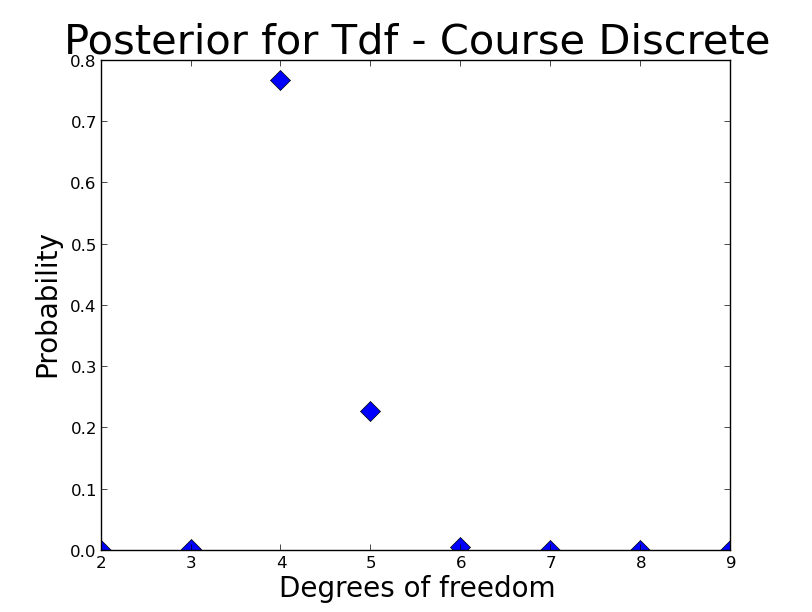
\includegraphics[width=\textwidth]{TdfCourseDiscPost}
        \end{subfigure}
        ~ 
        \begin{subfigure}[b]{0.31\textwidth}
                \centering
                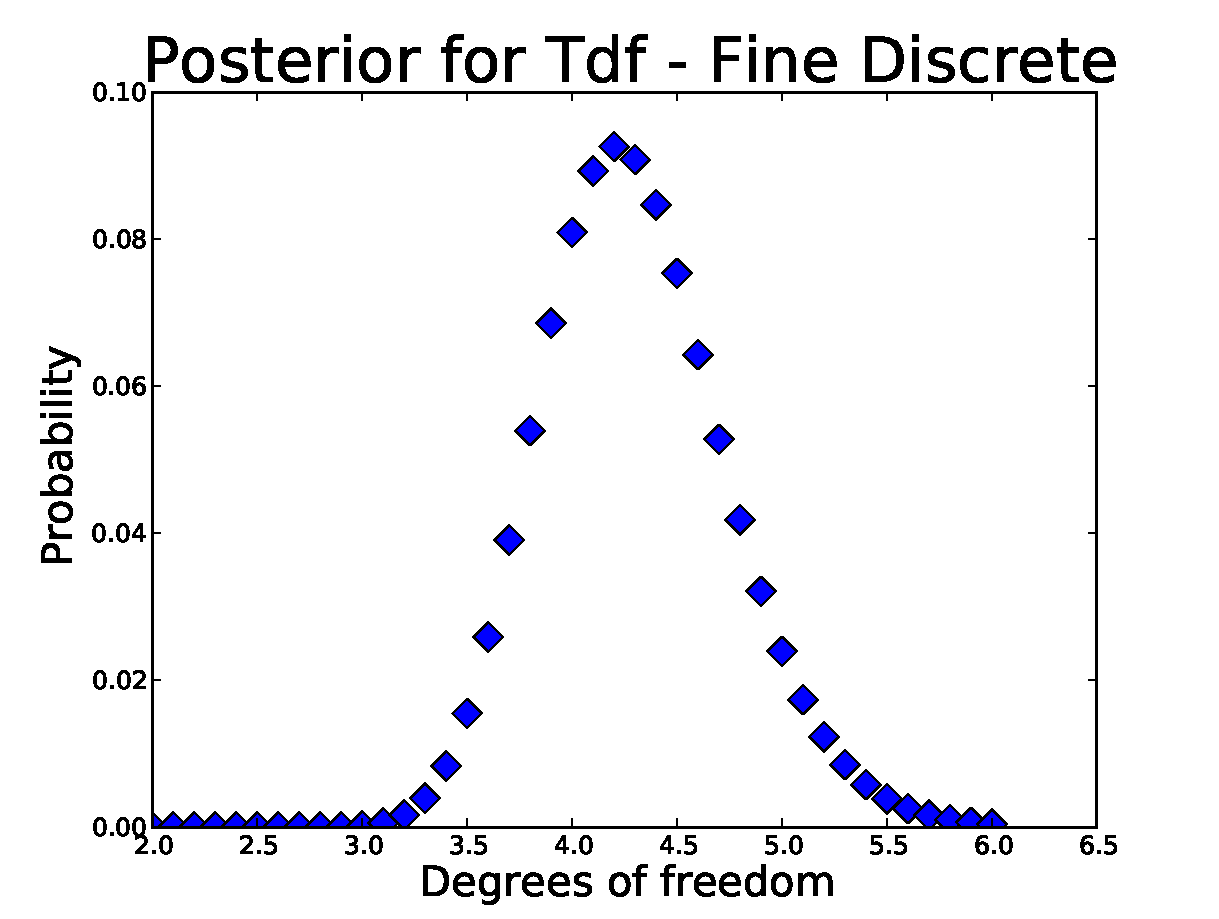
\includegraphics[width=\textwidth]{TdfFineDiscPost}
        \end{subfigure}
        ~ 
        \begin{subfigure}[b]{0.31\textwidth}
                \centering
                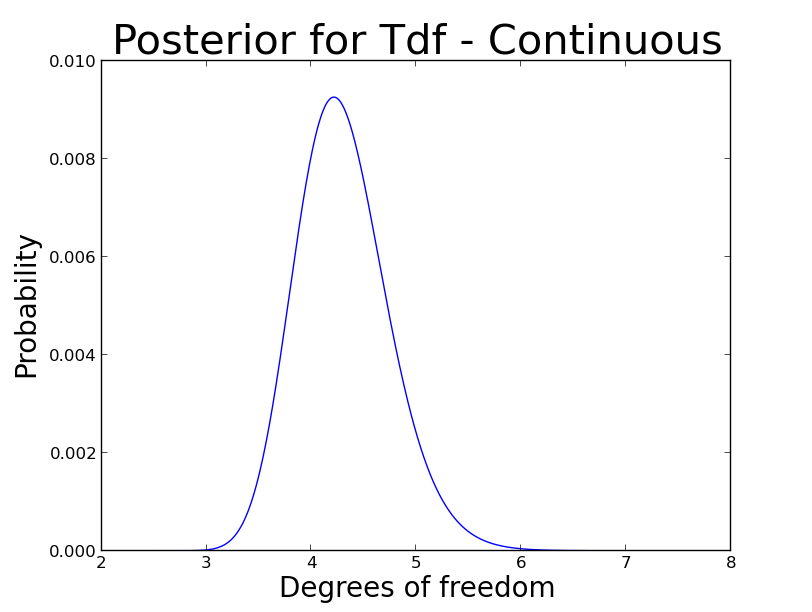
\includegraphics[width=\textwidth]{TdfContPost}
        \end{subfigure}
    \caption{True posterior distributions for the 3 Tdf models.}
    \label{fig:tdfPosts}
\end{figure}

\subsection{Tdf model results}
\todo{Add KL and KS difference results for these distributions}

On the course discrete model (Figure \ref{fig:tdfCourseDiscSamp}) we see that the two PPLs obtain similar results but with a large gap in runtime. Venture runs $\sim$54 time more slowly than OpenBUGS. To get a better idea of the relative performance of the languages we can look at their speed of convergence to the true posterior.

\begin{figure}[h]
    \centering
    \begin{subfigure}[t]{0.48\textwidth}
      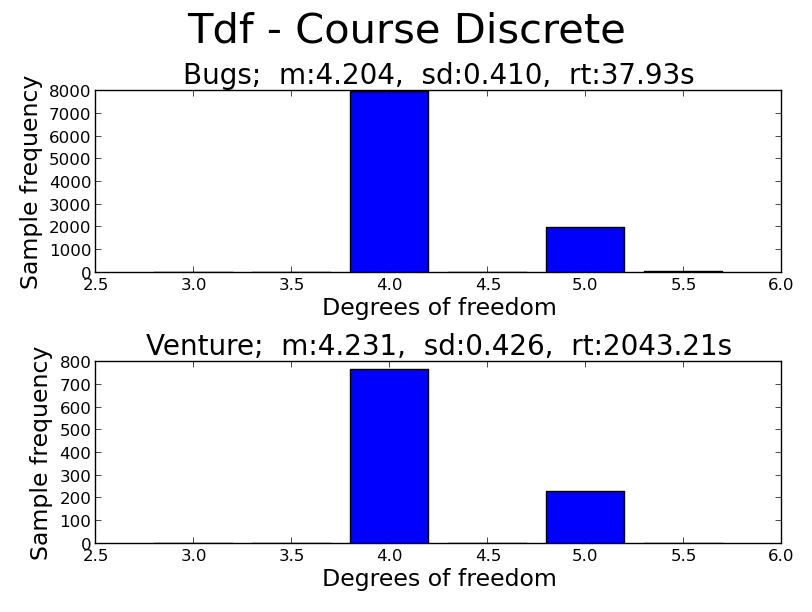
\includegraphics[width=\textwidth]{TdfCourseDiscSamps}
      \caption{Distributions obtained by the two PPLs on the course discrete model.}
      \label{fig:tdfCourseDiscSamp}
    \end{subfigure}
    ~
    \begin{subfigure}[t]{0.48\textwidth}
      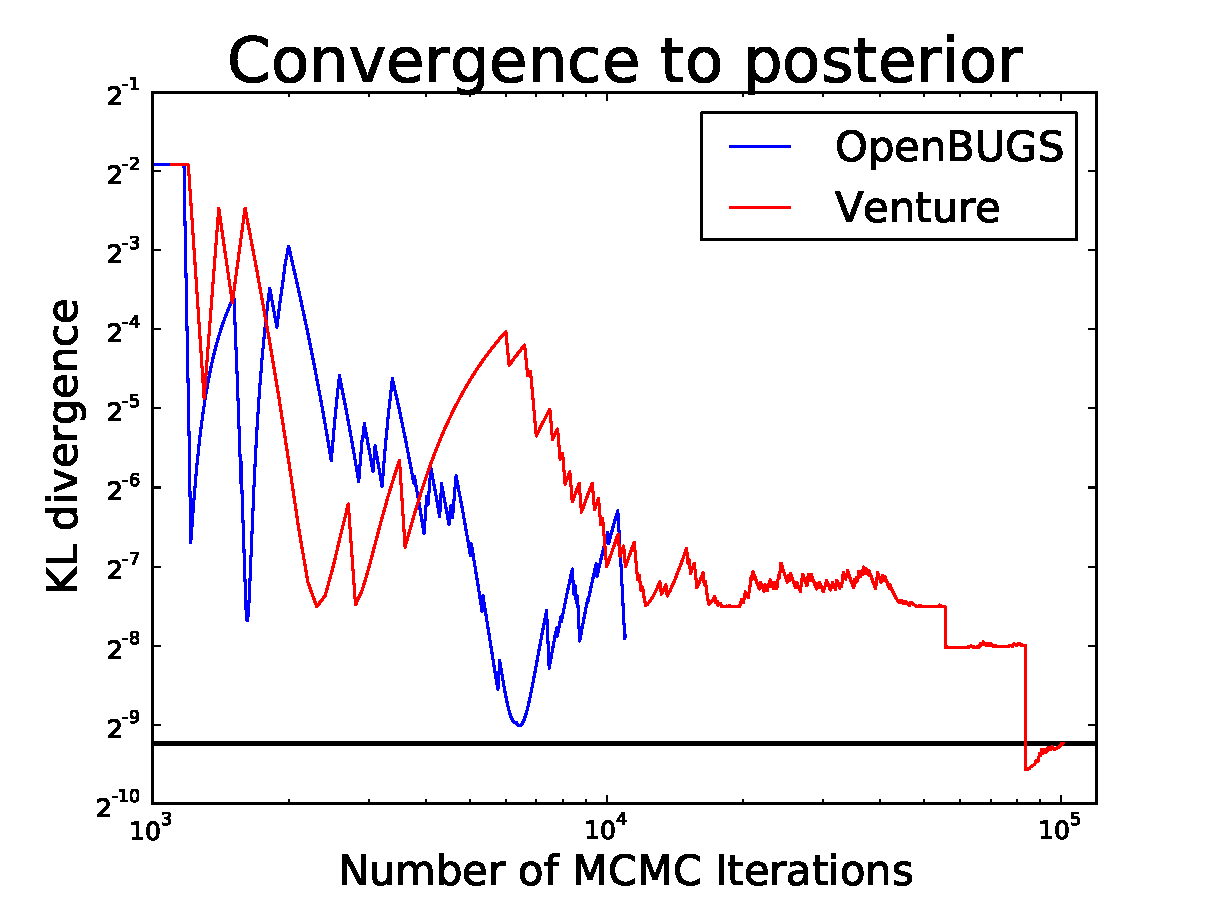
\includegraphics[width=\textwidth]{TdfCourseDiscConv}
      \caption{Rate of convergence of the two engines as the number of samples increases (first 1,000 samples are discarded as burn-in). The black line shows the KL divergence achieved by Venture after 101,000 inference steps.}
      \label{fig:tdfCourseDiscConv}
    \end{subfigure}
    \caption{Performance of the Tdf course discrete model}
\end{figure}

As seen in Figure \ref{fig:tdfCourseDiscConv}, due to the course discrete prior, the convergence rate here is quite choppy and no significant conclusions can be drawn from this single run. 

\todo{Maybe do more runs and plot quartiles}

\begin{figure}[h]
    \centering
    \begin{subfigure}[t]{0.48\textwidth}
      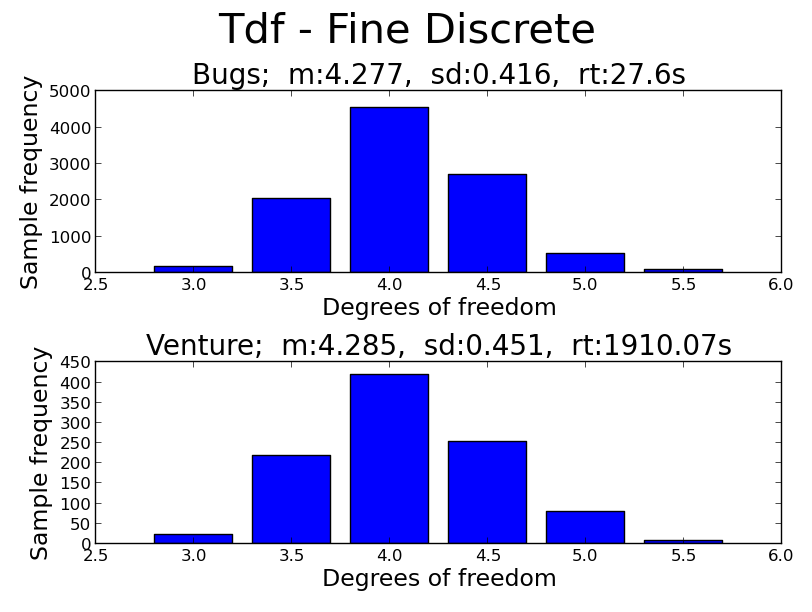
\includegraphics[width=\textwidth]{TdfFineDiscSamps}
      \caption{Distributions obtained by the two PPLs on the fine discrete model.}
      \label{fig:tdfFineDiscSamp}
    \end{subfigure}
    ~
    \begin{subfigure}[t]{0.48\textwidth}
      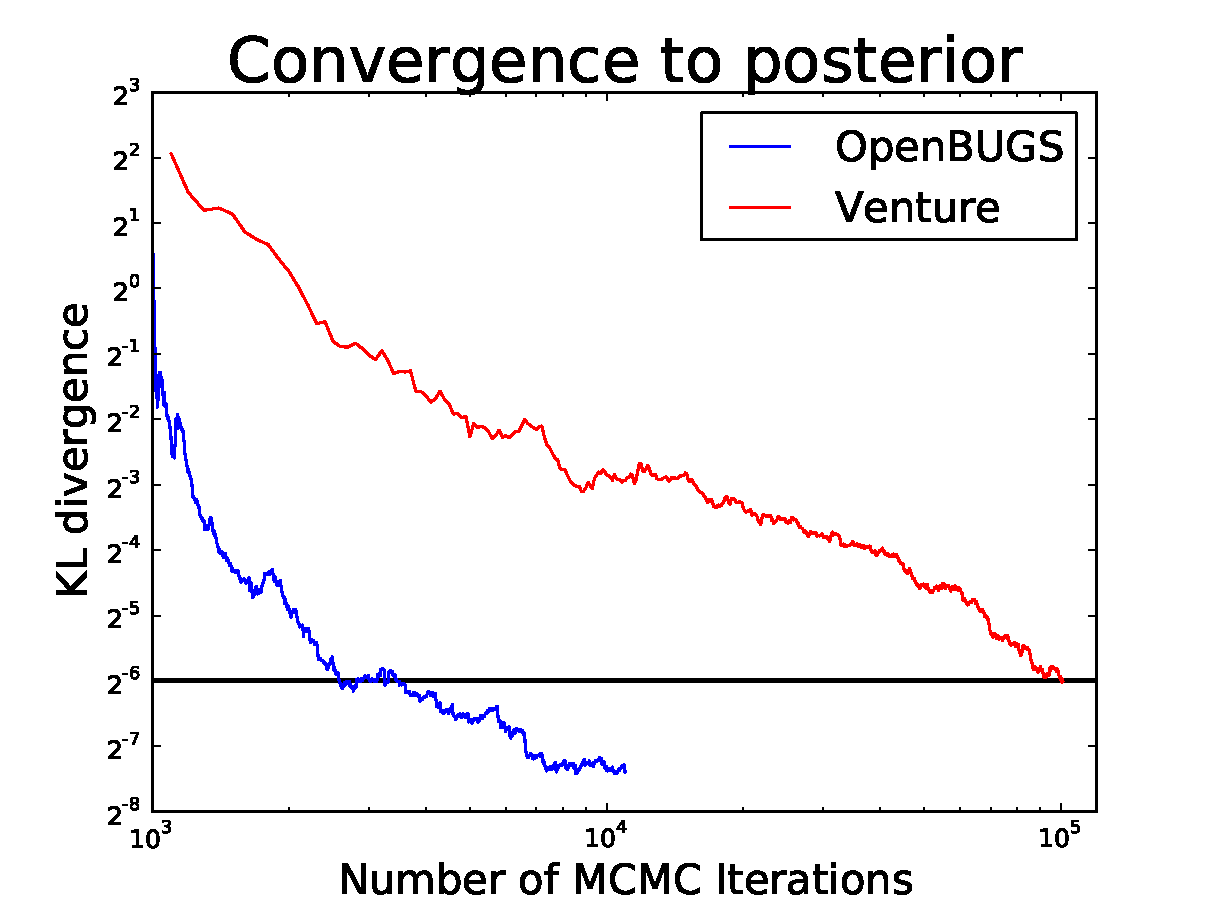
\includegraphics[width=\textwidth]{TdfFineDiscConv}
      \caption{Rate of convergence of the two engines as the number of samples increases (first 1,000 samples are discarded as burn-in). The black line shows the KL divergence achieved by Venture after 101,000 inference steps.}
      \label{fig:tdfFineDiscConv}
    \end{subfigure}
    \caption{Performance of the Tdf fine discrete model}
\end{figure}

Looking at the performance results on the fine discrete prior(see Figure \ref{fig:tdfFineDiscSamp}) shows that, as with the course discrete case, the two engines obtain similar looking distributions. Additionally, the runtime gap actually worsens here, Venture now having a runtime $\sim$69 times larger than OpenBUGS.

The convergence rate shown in Figure \ref{fig:tdfFineDiscConv} reveals that Venture also does a worse job of inferring the true posterior, despite the longer runtime. The finer prior used here results in a much smoother convergence rate and so we can see that the KL divergence reached by Venture after 101,000 samples is achieved by OpenBUGS after only 3,000 (including the burn-in). Performing 3,000 MCMC steps in OpenBUGS takes 8.7 seconds, while Venture's run took 1910. So we may say that, reported to convergence to true posterior, Venture is $1910/8.7 = \sim 220$ times slower than OpenBUGS.

\begin{figure}[h]
    \centering
    \begin{subfigure}[t]{0.48\textwidth}
      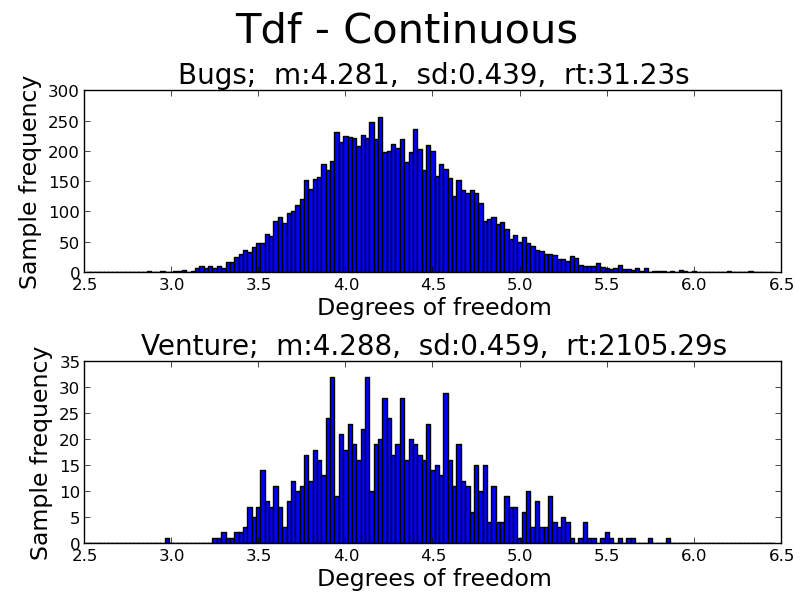
\includegraphics[width=\textwidth]{TdfContSamps}
      \caption{Distributions obtained by the two PPLs on the continuous model.}
      \label{fig:tdfContSamp}
    \end{subfigure}
    ~
    \begin{subfigure}[t]{0.48\textwidth}
      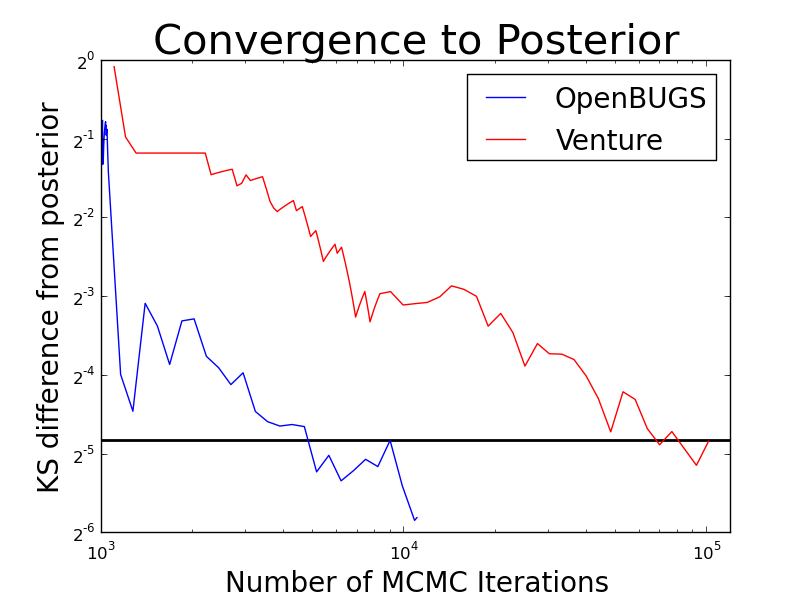
\includegraphics[width=\textwidth]{TdfContConv}
      \caption{Rate of convergence of the two engines as the number of samples increases (first 1,000 samples are discarded as burn-in). The black line shows the KS difference achieved by Venture after 101,000 inference steps.}
      \label{fig:tdfContConv}
    \end{subfigure}
    \caption{Performance of the Tdf continuous model}
\end{figure}

On the continuous case (see Figure \ref{fig:tdfContSamp}), not only does the runtime gap persist (Venture is again $\sim$68 times slower than OpenBUGS), but the distribution generated by Venture is also visibly noisier. One explanation for the noise could be the fact that, even though Venture is performing more MCMC iterations, due to the lag of 100 between extracted samples, it is actually generating only 1,000 samples compared to OpenBUGS' 10,000. 

The convergence rates presented in Figure \ref{fig:tdfContConv} show that, as with the fine discrete model, there seems to be a large qualitative gap between the performance of the two engines. Thus the KS difference achieved by Venture after 101,000 MCMC iterations is reached by OpenBUGS after only 5,000. Additionally, while Venture takes 2105 seconds to reach this performance level, OpenBUGS does it in 16.5. Venture is therefore $2105/16.5 = \sim 127$ times slower than OpenBUGS on this model.

Based on these results we can say that Venture performs significantly worse then OpenBUGS on the Tdf model variants (with the last two variants exhibiting a slow-down of more than 2 orders of magnitude).

\section{Analysis of Venture's performance}

In order to understand why Venture seems to perform so badly on the Tdf models, we look at the distribution of runs of identical samples generated by the two engines.

\begin{figure}[h]
    \centering
    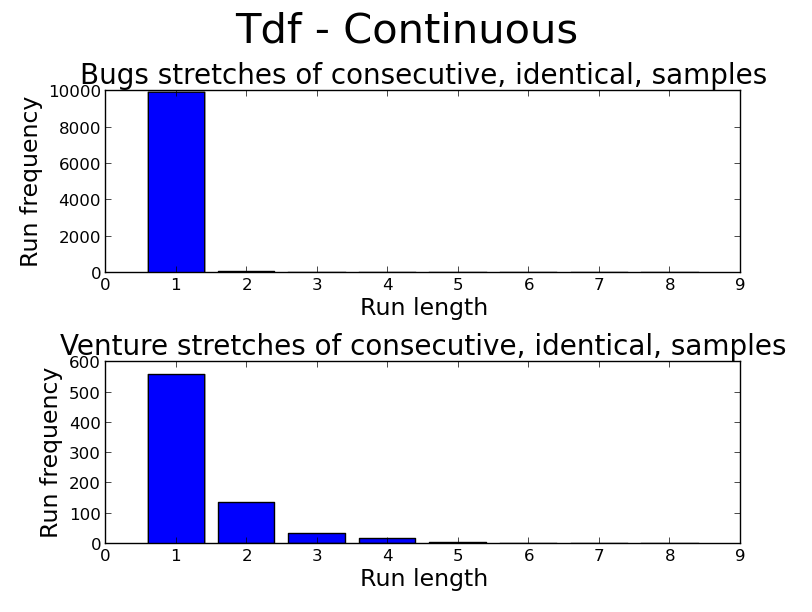
\includegraphics[width=\textwidth]{TdfContRuns}
    \caption{Number and size of identical sample runs generated by the two PPLs on the continuous model.}
    \label{fig:tdfContRun}
\end{figure}

Figure \ref{fig:tdfContRun} shows that Venture has a much higher propensity for identical sample runs than OpenBUGS. Keeping in mind that Venture takes a lag of 100 samples between each 2 extracted samples, we see that Venture exhibits several runs of over 500 MCMC iterations where the observed variable does not change at all. On the other hand, OpenBUGS has no two identical consecutive samples.

This difference can be explained by the different inference strategies employed by the two engines. Venture makes use of single-site Metropolis whereas OpenBUGS uses a slice sampler on one dimensional models such as Tdf \todo{saw this mentioned in a paper, need to find direct source or remove}. We take a closer look at these different inference techniques and their performance in Chapter \ref{chap:infEngines}.

\todo{Decide is there's anything worth reporting from the performance tests done on Venture. Log dates: 2014.02.19 and 2014.02.20}

\subsection{Webchurch's performance}
One alternative to Venture which I considered is WebChurch. WebChurch is a compiler which translated the Church PPL into JavaScript, and thus allows for in-browser execution.

I implemented a few very simple models (similar to the ones discussed below) in WebChurch, however the execution tended to hang even when conditioning on very few variables (less than 5) and when extracting very few samples (less than 100). Asking one of the WebChurch creators confirmed that the publicly available implementation is meant for didactic purposes and not designed to scale well. I therefore chose to focus only on Venture and OpenBUGS.

\chapter{Partitioned Priors}

In this chapter we look at a novel idea of improve the inference performance of basic Metropolis-Hastings by paritioning the prior distribution into several component parts. The idea behind this approach is that we may be able to guide the resampling process as to improve the rate of convergence to the mode and the mixing properties of local Metropolis-Hastings. \todo{say something about proposal kernels vs. sampling from prior?} If this approach proves succesful, it would enable us to design a light pre-inference rewriting of a probabilistic program which splits up its priors so that the subsequent inference step is performed more efficiently.

In the first instance, we focus on the splitting of uniform continuous priors. Not only are such priors commonly used in models, but sampling from any distribution ultimately relies on uniformly drawn random bits. Speeding up inference on uniform priors may therefore lead to speed ups on other distributions, assuming certain desirable properties, such that small changes in the uniform bits correspond to small changes in the final distribution. \todo{not sure if this makes much sense. Need to research it or remove}

For simplicity, we focus on models with a uni-modal posterior distribution. The analysis for multi-modal distributions would follow similar lines to the one presented here, but would also have to additionally account for mode-switching.

\section{Preliminaries}

In order to explore the partitioned prior idea we need to have an understanding of the basic Metropolis-Hastings algorithm. We also need a way to evaluate the performance of a certain partition, which we propose to do by looking separately at the time it takes for our Markov Chain to reach the true posterior's mode and at the chain's mixing properties around this mode. Finally, we can also consider the empirical distributions created by a fixed number of samples, which can be compared to a ground-truth distribution which is computer analytically. We perform this comparison by taking either the Kullback–Leibler divergence \cite{kullback1951information} (in the case of discrete distributions) or the Kolmogorov–Smirnov distance \cite{massey1951kolmogorov} (for continuous ones) between the correct posterior and the empirical distribution under consideration. 

\subsection{Metropolis-Hastings}
\label{sect:MH}
The Metropolis-Hastings algorithm is a method of drawing samples from a probability distribution $P(x)$ when we can only compute values of the proportional function $P^*(x) = P(x)*Z$ \cite{metropolis1953equation, hastings1970monte}. This method is usefull when we want to estimate distributions (or expectations under distributions) that we cannot directly evaluate, which is a common problem in Bayesian modeling, since the probability distribution's normalization factor is often difficult to estimate.

Metropolis-Hastings is a Markov Chain Monte Carlo algorithm, which is to say that the algorithm will generate samples according to the Markov, memoryless, property where the choice of current sample depends only on the previous sample. Additionally, the markov chain implied by this sequence of samples will have $P(x)$ as its stationary distribution. This implies that, if we run metropolis-hastings long enough for the underlying markov chain to be sampling from it's stationary distribution, then we will be drawing samples from $P(x)$.

In order to create an underlying markov chain that has $P(x)$ as its stationary distribution it is usefull to split the state transition into two components, a proposal function and an acceptance probability. Since we must respect the Markov, memoryless, property, the proposal function can only take the current sample as its input and is therefore of the form $Q(x_{n+1} | x_{n})$. It can then be shown \cite{neal1993probabilistic} that in order for the markov chain to converge to the right distribution, it is sufficient to define the acceptance ratio for as:
\[ \alpha = \frac{P(x_{n+1})}{P(x_{n})}\frac{Q(x_{n} | x_{n+1})}{Q(x_{n+1} | x_{n})} = \frac{P^*(x_{n+1})}{P^*(x_{n})}\frac{Q(x_{n} | x_{n+1})}{Q(x_{n+1} | x_{n})} \]

For the purpose of inference in probabilistic programming languages, a simplification to the Metropolis-Hastings algorithm is usually made by assuming that the proposal kernel is symmetric: $Q(x_{n+1} | x_{n}) = Q(x_{n} | x_{n+1}) \forall x_{n+1}, x_{n}$, which leads to removing the 2nd term for the acceptance ration. The full algorithm can then be described as:

\begin{flalign*}
&\text{1 Pick a first sample }x_0 &\\
&\text{2 Pick a proposal kernel }Q(x_{t+1} | x_{t}) &\\
&\text{3 Pick a desired number of samples to extract } N &\\
&\text{4 For t=0; t<N; t++} &\\
&\text{4.1 \quad\quad Generate proposal }prop \sim Q(x_{t+1} | x_{t}) &\\
&\text{4.2 \quad\quad Calculate acceptance ratio } \alpha = \frac{P^*(prop)}{P^*(x_{t})} &\\
&\text{4.3 \quad\quad Sample a uniformly random number } r \sim \text{(uniform-continuous 0 1)} &\\
&\text{4.4 \quad\quad Decide whether to accept the proposal } 
  \left\{
	  \begin{array}{ll}
      x_{t+1} = prop \text{, if } r < \alpha \\
      x_{t+1} = x_{t} \text{, otherwise}
	  \end{array}
  \right. &\\
\end{flalign*}

Intuitively we can see that the acceptance ratio checks how likely the proposal is in comparison to the current sample. If the proposal is more likely it is always accepted. Otherwise it is accepted with a probability that decreases the more unlikely the proposal is. In this way, the markov chain will have a chance to explore less likely probability regions while preferring to stay in the high-density areas.

For a more thorough discussion of Metropolis-Hastings, including proofs, please see \cite{mackay2003information, neal1993probabilistic}.

\subsection{Expected number of iterations to a neighbourhood of the mode}
\label{section:sampsToMode}
The first test of the efficiency of a partition is, on average, how many iterations the algorithm will have to go through before the markov chain reaches a state close to the mode of the posterior. Since we are interested in seeing our markov chain mix around the posterior's mode, we want it to get close to the mode as soon as possible. The average number of iterations to the mode can also be viewed as a way to estimate a lower bound on the burn-in we should set for our algorithm.

When using local Metropolis-Hastings with an unpartitioned uniform prior, it is easy to analytically calculate the expected number of iterations to a mode's neighbourhood. Using the unpartitioned prior (uniform-continuous a b), we end up sampling from the uniform distribution and accepting or rejecting those samples according to the Metroplis-Hastings acceptance ratio. In order to reach some neighbourhood of the mode $[mode - \epsilon, mode + \epsilon]$, we need to actually sample a number in that range from the prior (sample which will definitely be accepted since it will have higher log likelihood than anything outside that range). This means the number of samples it will take to get close to the mode with an unpartitioned prior will follow a geometric distribution with $p = (2\epsilon)/(b-a)$. The expected number of samples it takes to reach the neighbourhood will then be $(b-a)/(2\epsilon)$.

For partitioned priors it will usually not be possible to analytically determine the expected number of steps to $[mode - \epsilon, mode + \epsilon]$, so we shall instead perform empirical tests.

\subsection{Mixing properties around the mode}
Once the markov chain has reached the mode we wish to see how well it manages to mix around it. Here we look at different metrics that might give us an idea of the mixing properties. Visually inspecting the sample evolution will show if the inference tends to get stuck on certain values for long stretches. A numerical estimate of this can be obtained by measuring the ''distance'' traveled by the markov chain around the mode (i.e. the sum of absolute differences between consecutive samples). We can also inspect the sample autocorrelation, based on the idea that good mixing should imply a small autocorrelation within a sample run.

\section{Sum of uniforms}
\label{sect:sumUnif}

We first consider partitioning the uniform prior into a sum of uniforms. This choice is made both for simplicity and so that we can observe some basic properties concerning local Metropolis-Hasting's performance on partitioned priors.

Such a partitioning, however, should not be used in actual probabilistic program compilation techniques since it does not leave the prior invariant (that is to say, a sum of uniform variables is not a uniform variable, see Figure \ref{fig:1295Prior}). The invariance is due to the uniform distribution not being infinitely divisible. The approach presented in this section could be safely used on other distributions, such as Gammas and Gaussians, which are infinitely divisible. In Section \ref{sect:bitDecomp} we will present a partitioning technique which does leave the uniform prior unchanged.

\begin{figure}[h]
    \centering
    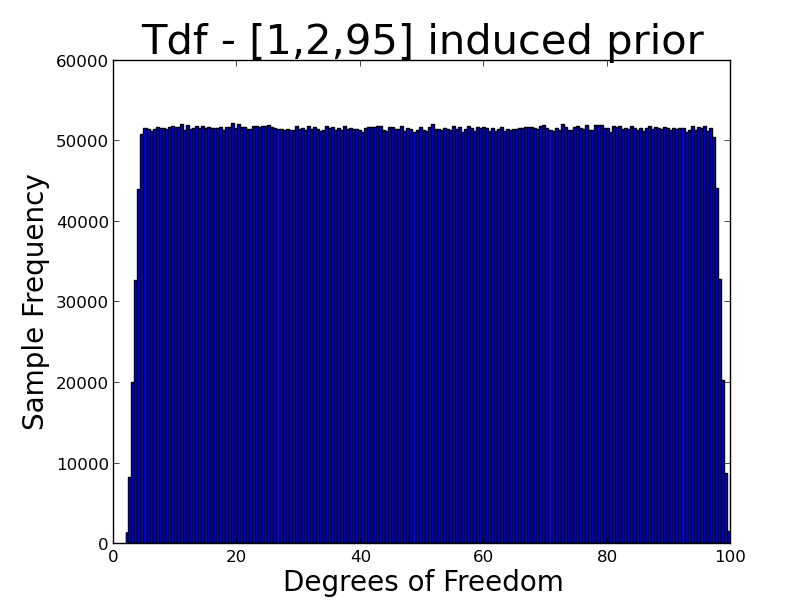
\includegraphics[width=0.8\textwidth]{Tdf1295Prior}
    \caption{Distribution induced by partitioning the prior (uniform-continuous 2 100) into (uniform-continuous 2 95) + (uniform-continuous 0 2) (uniform-continuous 0 1).}
    \label{fig:1295Prior}
\end{figure}

\subsection{Finding a good sum decomposition}
\label{sect:goodSum}
First we look at the expected number of steps needed to reach a neighbourhood of the mode. As explained in Section \ref{section:sampsToMode}, the expected number of steps to $[mode - \epsilon, mode + \epsilon]$ can be analytically computed for the unpartitioned prior (uniform-continuous a b) as $(b-a)/(2\epsilon)$.

For the partitioned priors, we instead perform empirical tests. These tests measure how many samples it takes for different partitions to reach mode neighbourhoods of different sizes. One thousand runs are done for each partition and neighbourhood sizes of of 1, 0.5, 0.2 and 0.02 are considered. The partitions consist of between 2 and 5 values which were drawn with replacement from [0, 0.5, 1, 2, 5, 7, 10, 15, 20, 25, 30, 35, 40, 45].

Table \ref{tab:bestParts} contains the empirical performance for the unpartitioned prior and for the best 2 partitions on each neighbourhood size. We specify partitions in the format (x,y,z) meaning (uniform-continuous 0 x) + (uniform-continuous 0 y) + (uniform-continuous 2 z). All considered partitions respect the constraint $x+y+z = 98$, so that the sum of all the component samples will be in the [2, 100] range specified by the uniform prior of the Tdf model, (uniform-continuous 2 100). 

\begin{table}[h]
  \centering
  \begin{tabular}{lllll}
    \toprule
    \multirow{2}{*}{Partition} & \multicolumn{4}{l}{Target neighbourhood size} \\
    \cmidrule(r){2-5} 
    & 1 & 0.5 & 0.2 & 0.02 \\
    \midrule
    Unpartitioned & 98.38 & 199.29 & 494.87 & 4919.75 \\
    (5, 93) & 89.03 & 122.87 & 172.9  & 670.14 \\
    (20, 78)& 92.55 & 142.6  & 259.21 & 1834.18 \\
    (2, 96) & 92.56 & 117.35 & 157.83 & 371.9 \\
    (1, 45, 52) & 123.97 & 146 & 172.78 & 400.01 \\
    (0.5, 2, 95.5) & 134.24 & 162.03 & 201.57 & 297.79 \\
    (1, 2, 95) & 130.06 & 155.48  & 186.83 & 317.31 \\
    \bottomrule
  \end{tabular}
  \caption{Expected number of steps to mode neighbourhoods on the Tdf continuous model for an unpartitioned prior and some of the best sum decomposition priors.}
  \label{tab:bestParts}
\end{table}

The best partition depends on the size of the neighbourhood, but we can observe partitions that consistently and significantly outperform the unpartitioned prior on all the neighbourhood sizes looked at above. In fact, for epsilon values of 0.1 and 0.01 the unpartitioned prior performs worse than any of the partitioned variants. Additionally, as epsilon gets smaller, it becomes useful to have smaller partition components. This leads to the 0.5 partition appearing in the best solution for a mode neighbourhood of size 0.02, but not in any of the top solutions for larger neighbourhoods.

The second aspect of convergence that a partition might help with is the mixing rate around the mode. In order to test the priors' mixing properties we need to consider what happens after the markov chain reaches the mode. We do this by setting the initial sample to the mode of the true posterior distribution and checking how much the chain moves over the next 1000 samples. Repeating this test 100 times and averaging the sum of absolute jump distances gives us the results in Table \ref{tab:partMix}.

\begin{table}[h]
  \centering
  \begin{tabular}{lll}
    \toprule
    Partition & Mean distance travelled & Variance in distance travelled \\
    \midrule
    Unpartitioned & 7.75 & 13.43 \\
    (1, 1, 1, 95) & 137.55 & 393.96 \\
    (1, 1, 1, 1, 94) & 135.08 & 616.41 \\
    (1, 1, 2, 94) & 131.19 & 539.03 \\
    (1, 1, 1, 2, 93) & 129.91 & 583.16 \\
    (0.5, 1, 1, 1, 94.5) & 126.76 & 382.09 \\
    (1, 2, 95) & 125.67 & 408.16 \\
    (1, 1, 96) & 125.44 & 311.76 \\
    (0.5, 1, 2, 94.5) & 123.38 & 487.26 \\
    (1, 1, 2, 2, 92) & 122.9 & 615.54 \\
    (2, 2, 94) & 121.25 & 844 \\
    \bottomrule
  \end{tabular}
  \caption{Average distance travelled around the mode on the Tdf continuous model for an unpartitioned prior and some of the best sum decomposition priors.}
  \label{tab:partMix}
\end{table}

This test only measures the average distance travelled (i.e. sum of absolute differences between consecutive samples), which could be a misleading measure of mixing. However, the large difference between the unpartitioned and the partitioned variants do suggest that there is some improvement here. We perform further tests on the mixing rate in Section \ref{sect:1295Eval}.

Based on the above results, we decide to further investigate the performance of the (1, 2, 95) partitioned prior, since this decomposition performs well both in reaching the mode and in mixing around it.

\subsection{Evaluating the (1,2,95) sum decomposition}
\label{sect:1295Eval}

Table \ref{tab:bestParts} makes clear the increased speed in reaching a neighbourhood of the mode offered by the decompositions. The potential benefit conferred in mixing rate is less clear however. To test this we look at the sample evolution (Figure \ref{fig:tdfPSampEvol}) and autocorrelation plots (Figure \ref{fig:tdfPAutoCorr}) for two runs obtained with an unpartitioned and a (1,2,95) partitioned prior. These experiments confirm our preliminary results from Section \ref{sect:goodSum}, and show that the partitioned prior does help with mixing around the mode and with eliminating large correlations between consecutive samples. 

\begin{figure}[h]
    \centering
    \begin{subfigure}[t]{0.48\textwidth}
      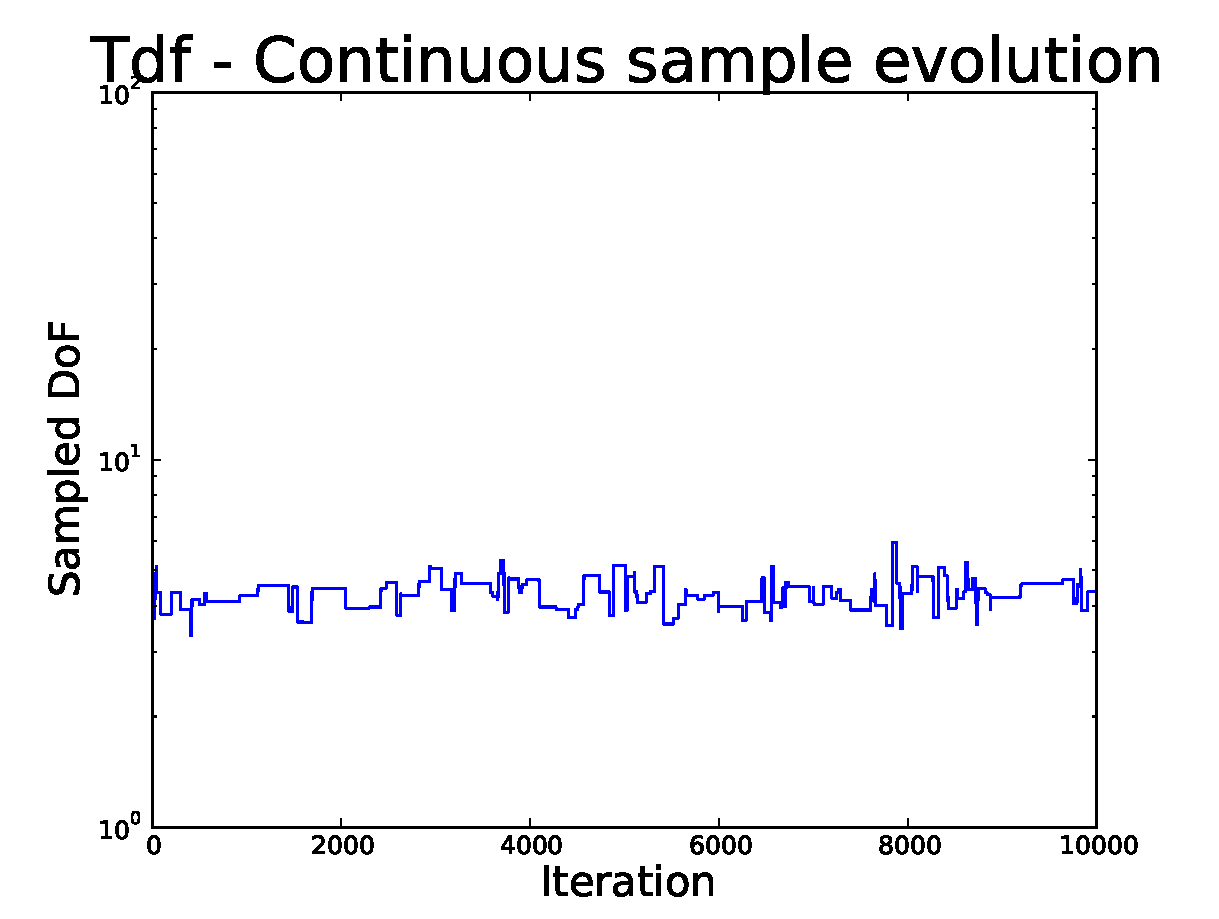
\includegraphics[width=\textwidth]{TdfSampEvol}
    \end{subfigure}
    ~
    \begin{subfigure}[t]{0.48\textwidth}
      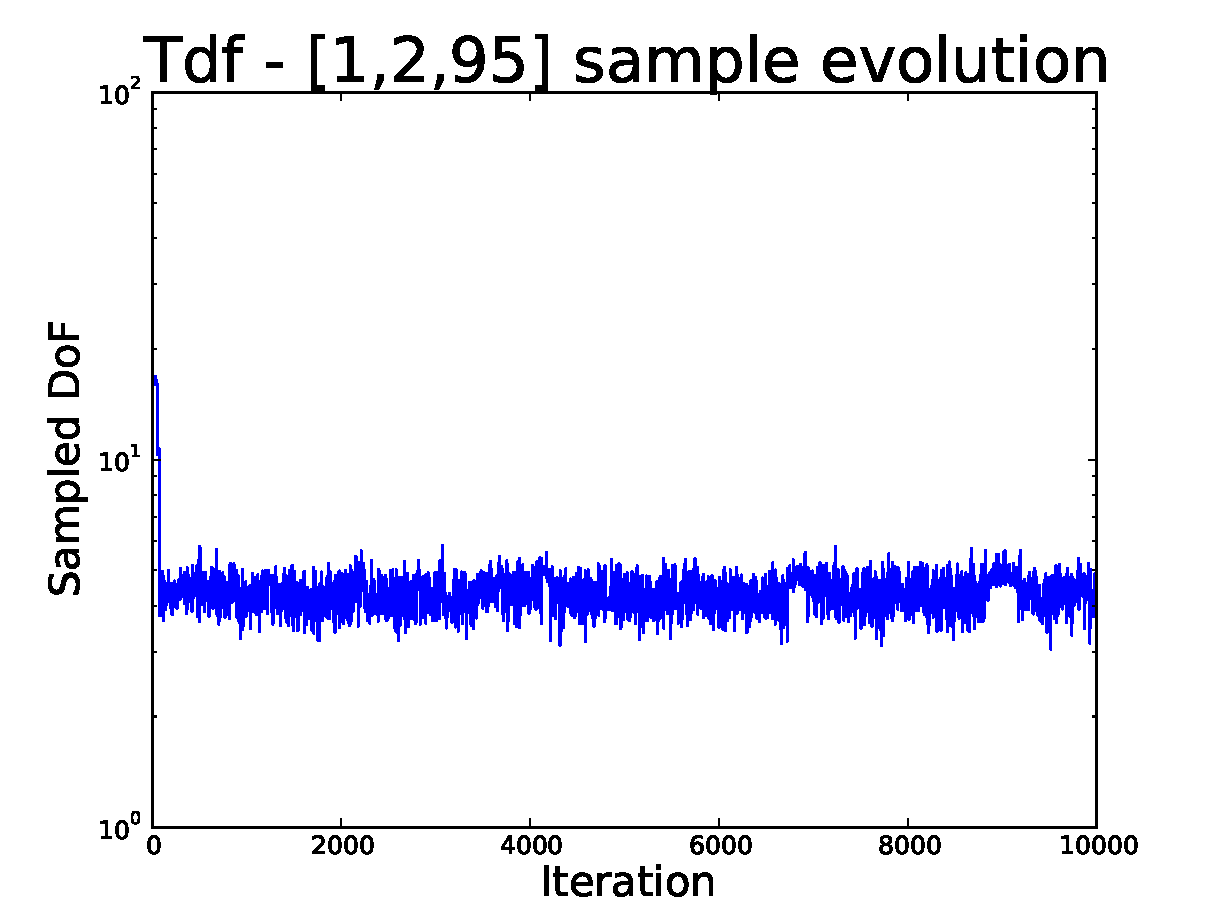
\includegraphics[width=\textwidth]{Tdf1295SampEvol}
    \end{subfigure}
    \caption{Sample evolutions for the unpartitioned and the (1, 2, 95) partitioned priors, over 10,000 samples on the Tdf continuous model.}
    \label{fig:tdfPSampEvol}
\end{figure}

\begin{figure}[h]
    \centering
    \begin{subfigure}[t]{0.48\textwidth}
      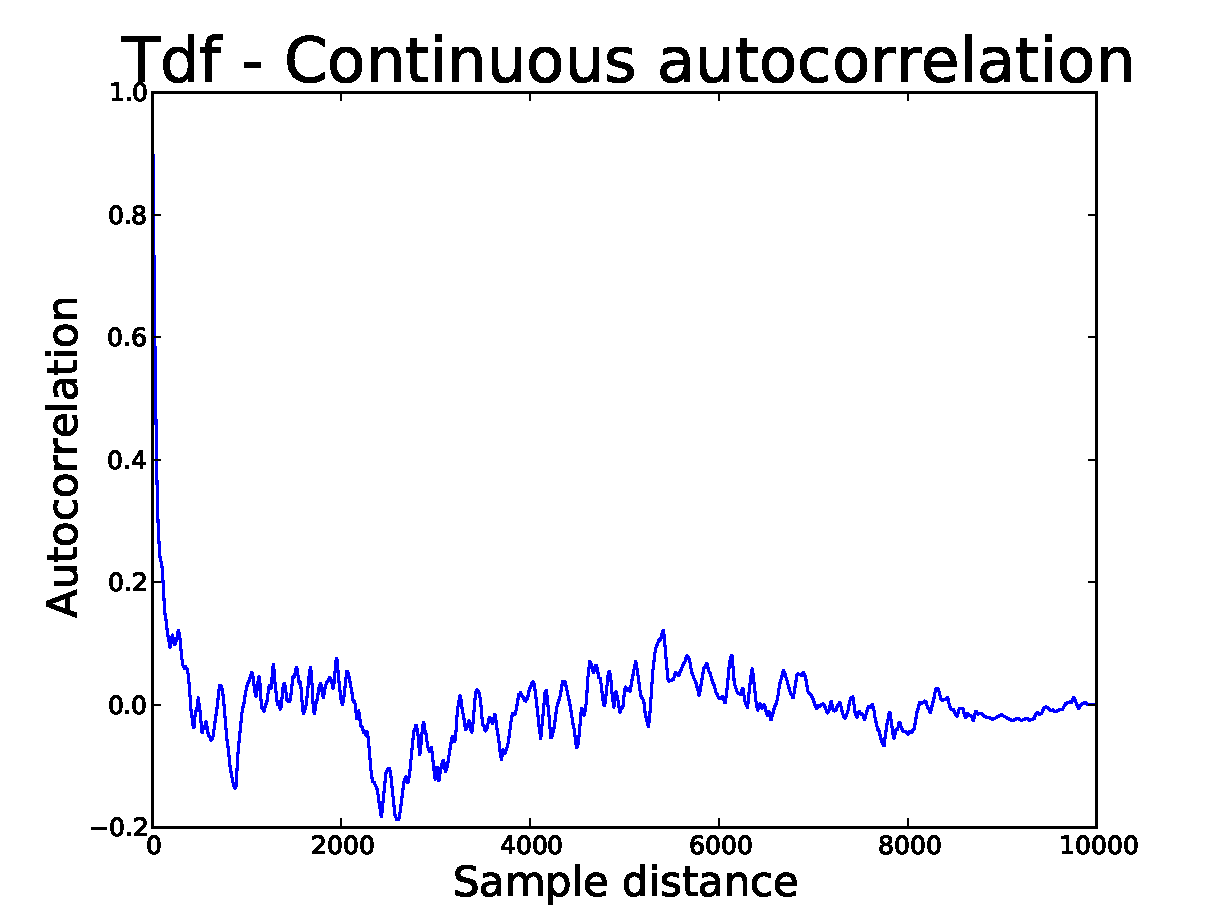
\includegraphics[width=\textwidth]{TdfAutoCorr}
    \end{subfigure}
    ~
    \begin{subfigure}[t]{0.48\textwidth}
      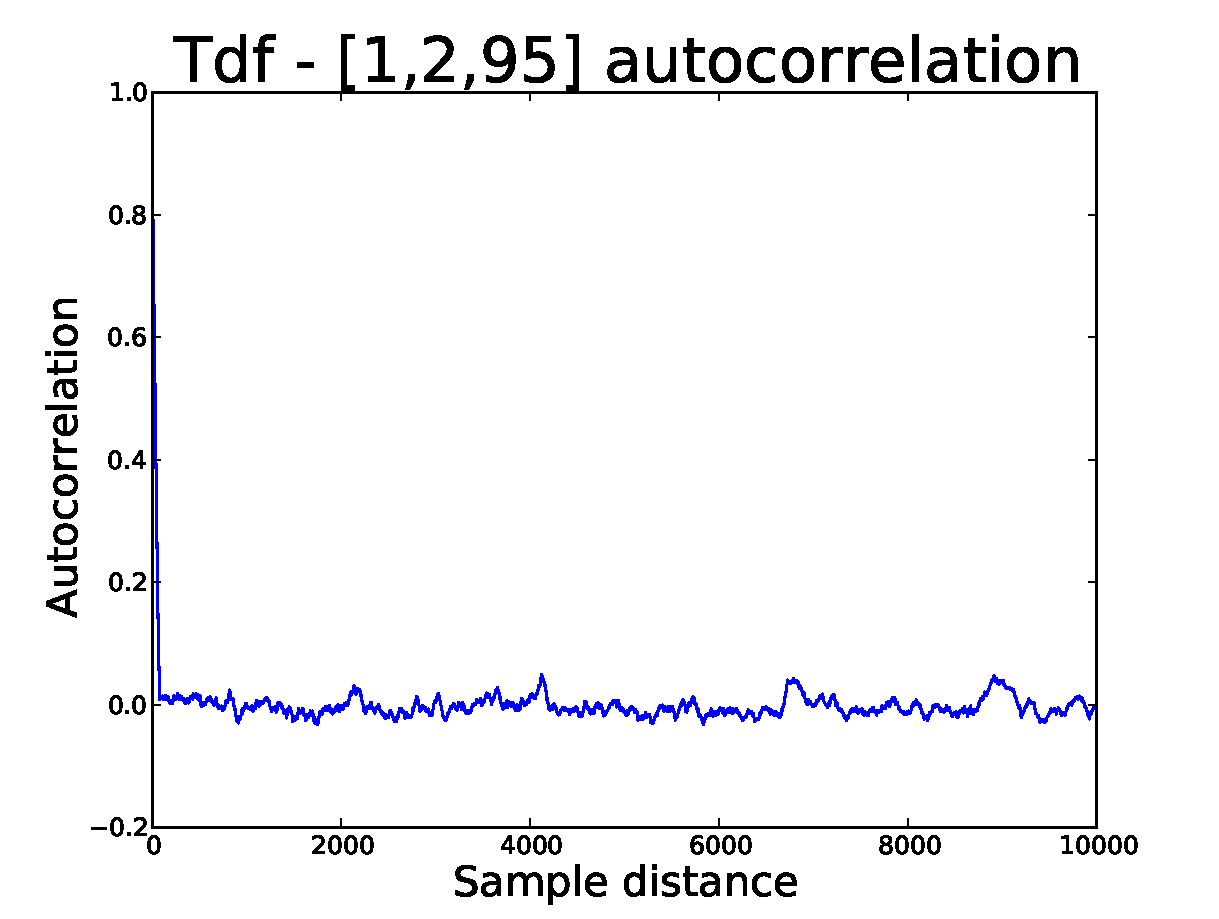
\includegraphics[width=\textwidth]{Tdf1295AutoCorr}
    \end{subfigure}
    \caption{Sample autocorrelations for the unpartitioned and the (1, 2, 95) partitioned priors, over 10,000 samples on the Tdf continuous model.}
    \label{fig:tdfPAutoCorr}
\end{figure}

The final test in determining the quality of the decomposition is to look at the actual sample distributions obtained under the two different prior formulations . For convenience, the true posterior for the Tdf continuous model is shown again in Figure \ref{fig:tdfPLL}. Looking at the sample distributions in Figure \ref{fig:tdfPDist} it is quite clear the partitioned prior outperforms the original, unpartitioned, variant. However, this result may be misleading since we are evaluating it on the same distribution which we used to choose the form of the partition. To test the robustness of our partition we repeat the above tests on a new model.

\begin{figure}[h]
    \centering
    \begin{subfigure}[t]{0.48\textwidth}
      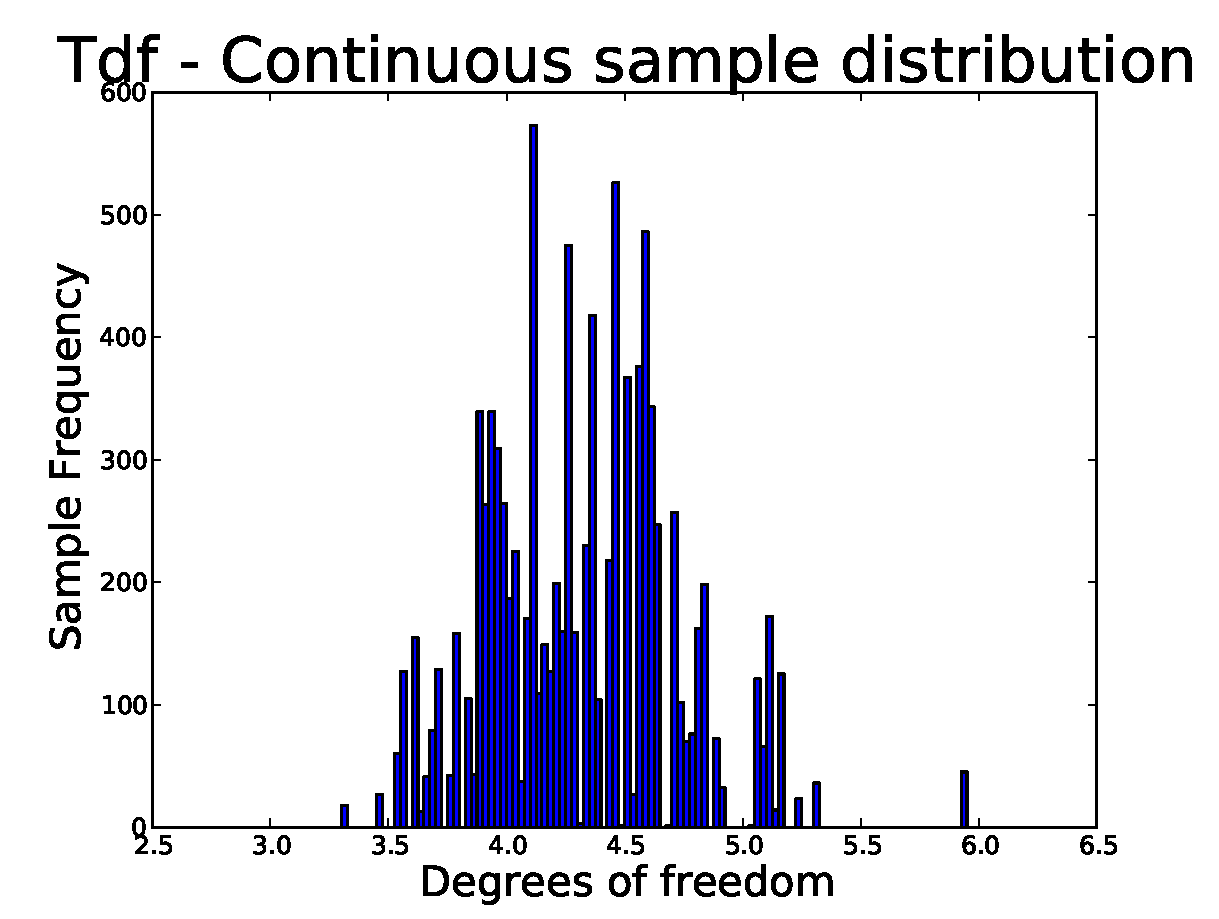
\includegraphics[width=\textwidth]{TdfSampDist}
    \end{subfigure}
    ~
    \begin{subfigure}[t]{0.48\textwidth}
      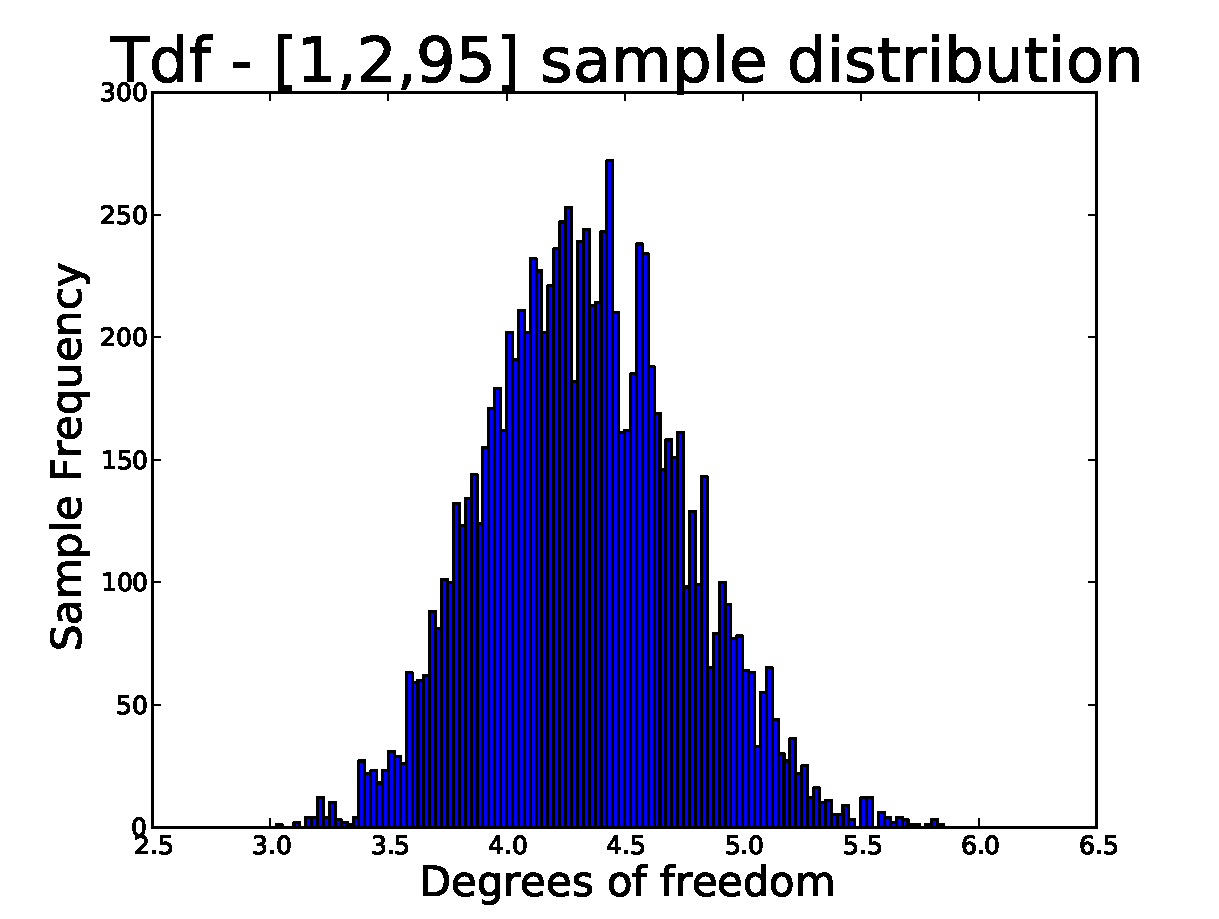
\includegraphics[width=\textwidth]{Tdf1295SampDist}
    \end{subfigure}
    \caption{Sample distributions for the unpartitioned and the (1, 2, 95) partitioned priors, over 10,000 samples on the Tdf continuous model.}
    \label{fig:tdfPDist}
\end{figure}

\subsubsection{The Tdf21 model}
In order to test our decomposition on a different posterior distribution, we generate 1,000 datapoints from a Student t distribution with 21 degrees of freedom and condition the Tdf Continuous model on this new dataset. The resulting posterior is shown in Figure \ref{fig:tdfPPost}. The mode here is actually 11.5. This is probably due to the fact that 1000 datapoints are not enough to accurately pinpoint a student-t with so many degrees of freedom (21) since, as the number of degrees of freedom increases, the differences between corresponding student-t distributions shrinks. The posterior distribution is however significantly different from the one for the previous dataset, which should be sufficient for testing the properties of the priors.

\begin{figure}[h]
    \centering
    \begin{subfigure}[t]{0.48\textwidth}
      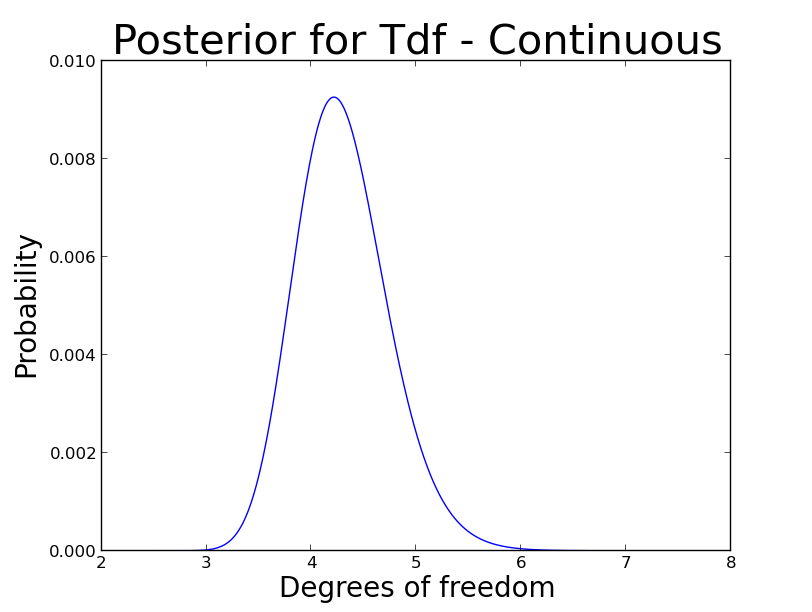
\includegraphics[width=\textwidth]{TdfContPost}
    \end{subfigure}
    ~
    \begin{subfigure}[t]{0.48\textwidth}
      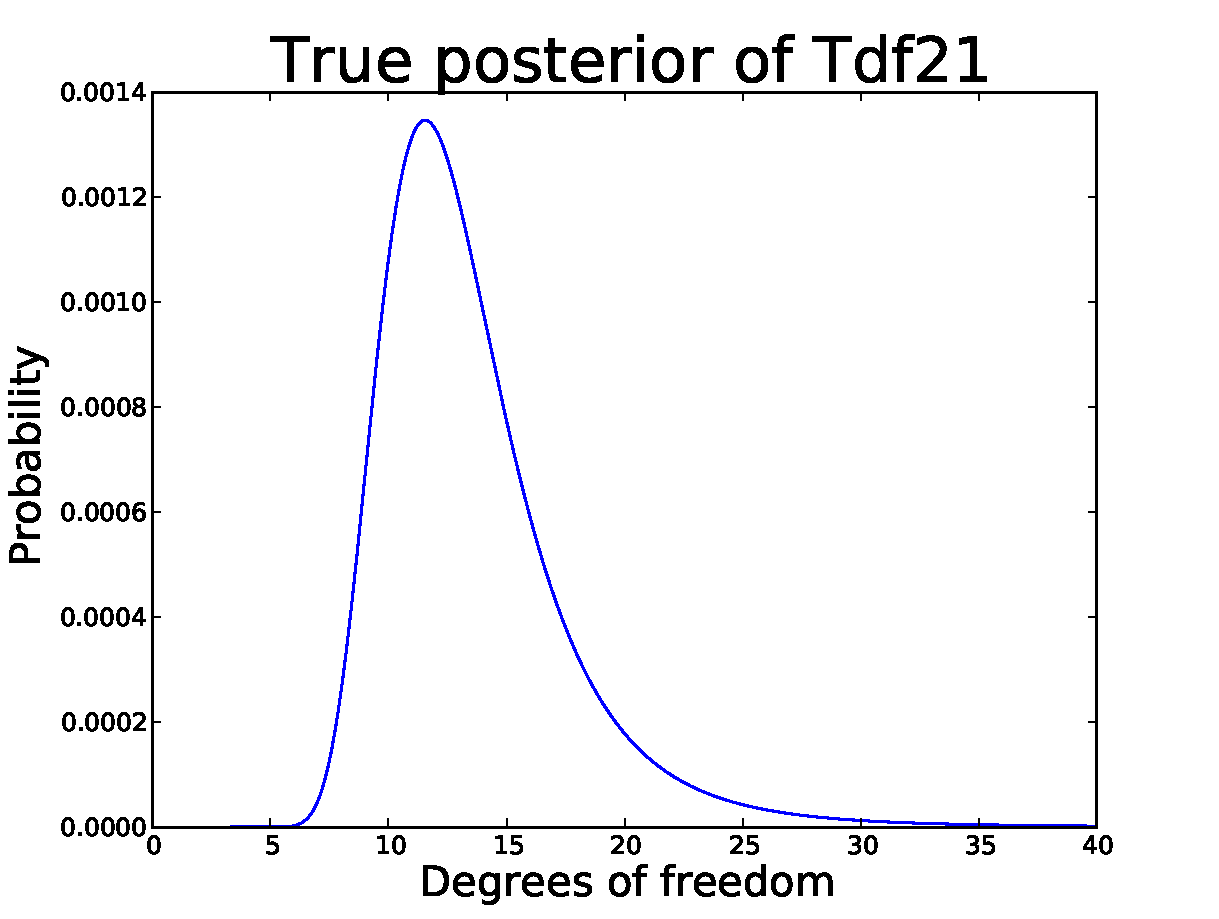
\includegraphics[width=\textwidth]{Tdf21Post}
    \end{subfigure}
    \caption{The true posteriors of the Tdf continuous and the Tdf21 continuous models.}
    \label{fig:tdfPPost}
\end{figure}

In order to better understand how the Metropolis-Hastings algorithm will be affected by this change, Figure \ref{fig:tdfPLL} also shows the log-likelihoods induced by the original Tdf Continuous model and by the Tdf21 continuous model. We can see that the Tdf21 log-likelihood is much flatter than the one for the original model. By repeating the mixing tests performed above we can test the effect of this difference.

\begin{figure}[h]
    \centering
    \begin{subfigure}[t]{0.48\textwidth}
      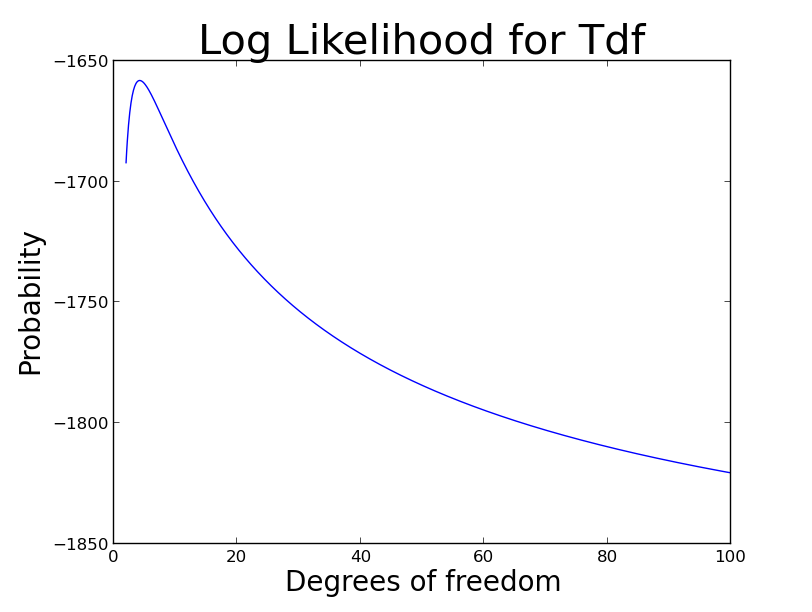
\includegraphics[width=\textwidth]{TdfContLL}
    \end{subfigure}
    ~
    \begin{subfigure}[t]{0.48\textwidth}
      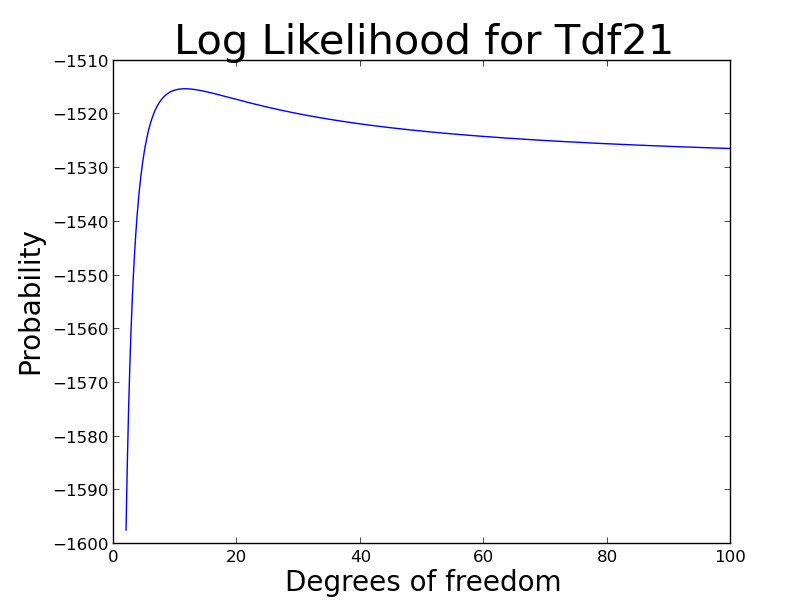
\includegraphics[width=\textwidth]{Tdf21LL}
    \end{subfigure}
    \caption{The true log-likelihoods of the Tdf continuous and the Tdf21 continuous models.}
    \label{fig:tdfPLL}
\end{figure}

\subsubsection{Evaluating the decomposition on the Tdf21 model}
We now test the convergence of the priors on the Tdf21 model by plotting the sample evolution, the sample autocorrelation and the sample distributions. The partitioned prior is the same one we used on the previous datapoints, namely (1,2,95). From the sample evolutions (Figure \ref{fig:tdf21PSampEvol}) we can see that the partitioned samples tend to clump a little more since bigger changes in the samples only occur when the 95 component changes. Both versions seem to mix well though.


\begin{figure}[h]
    \centering
    \begin{subfigure}[t]{0.48\textwidth}
      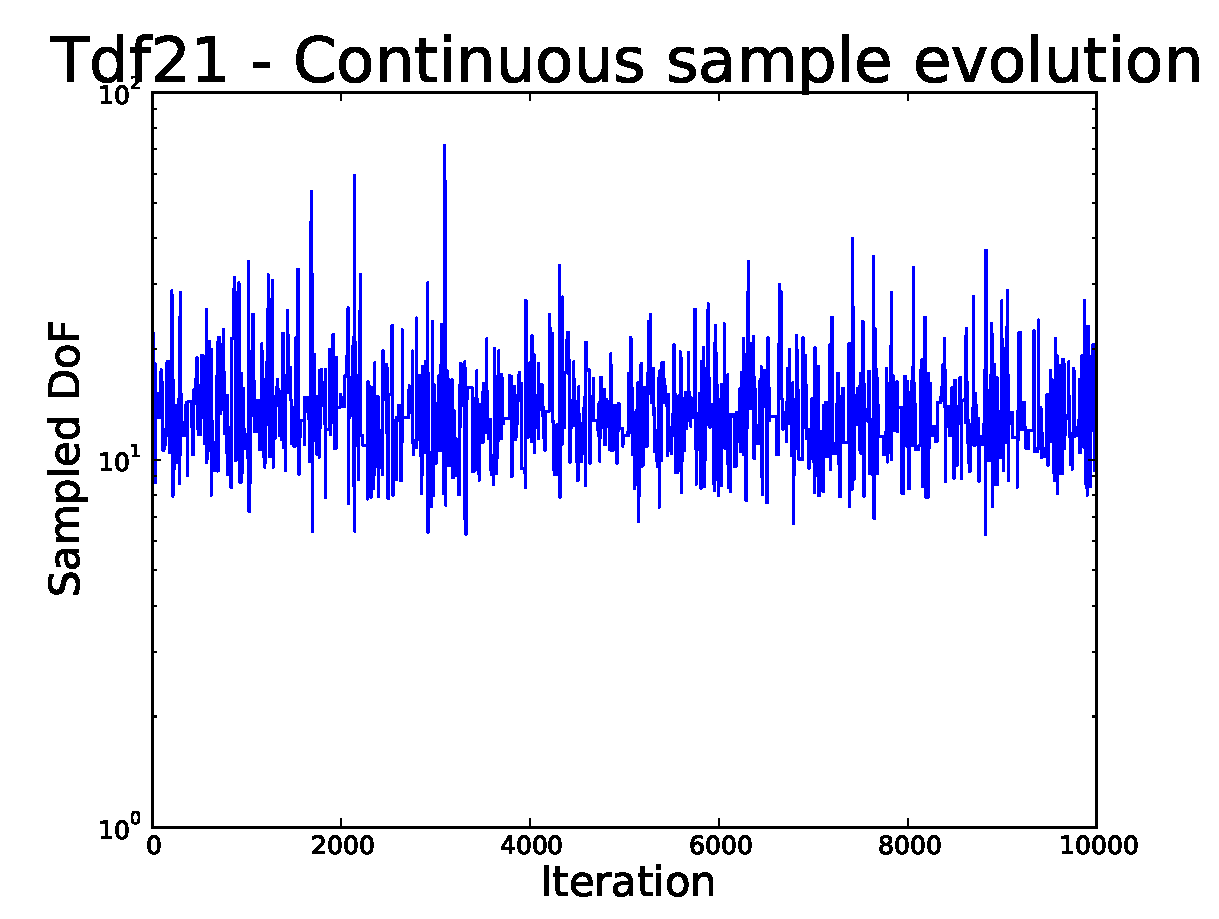
\includegraphics[width=\textwidth]{Tdf21SampEvol}
    \end{subfigure}
    ~
    \begin{subfigure}[t]{0.48\textwidth}
      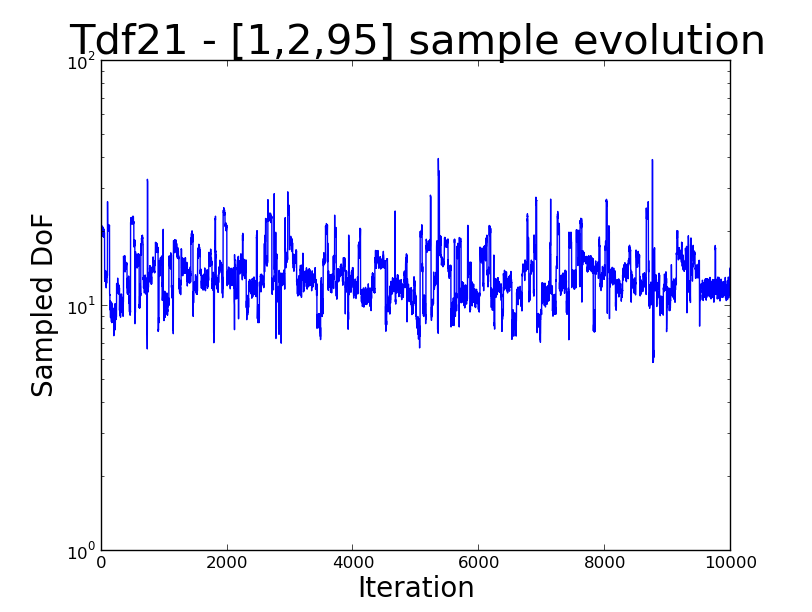
\includegraphics[width=\textwidth]{Tdf211295SampEvol}
    \end{subfigure}
    \caption{Sample evolutions for the unpartitioned and the (1, 2, 95) partitioned priors, over 10,000 samples on the Tdf21 model.}
    \label{fig:tdf21PSampEvol}
\end{figure}

The autocorrelation plots shown in Figure \ref{fig:tdf21PAutoCorr} are also more similar than in the case of the original Tdf model. The unpartitioned prior does quite well here since the flat shape of the log-likelihood means there is a higher chance that a proposition drawn from the prior will be accepted by the Metropolis-Hastings algorithm.

\begin{figure}[h]
    \centering
    \begin{subfigure}[t]{0.48\textwidth}
      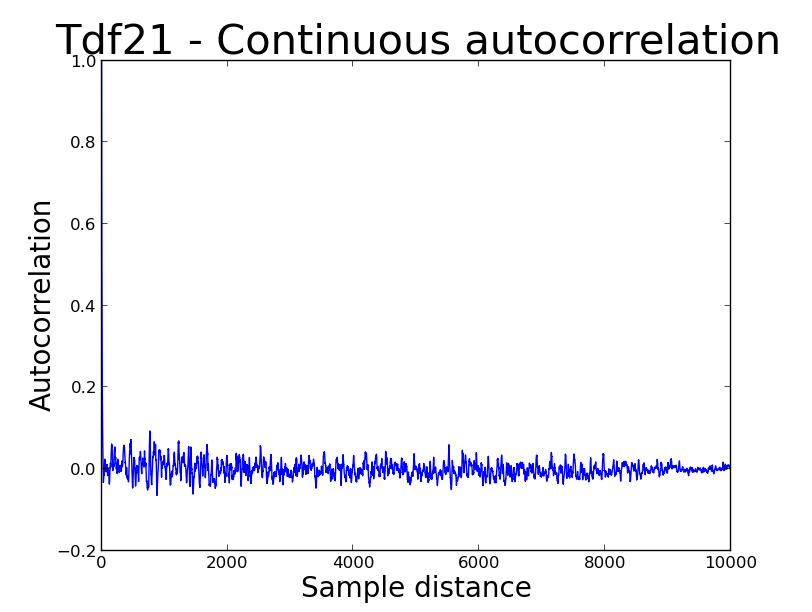
\includegraphics[width=\textwidth]{Tdf21AutoCorr}
    \end{subfigure}
    ~
    \begin{subfigure}[t]{0.48\textwidth}
      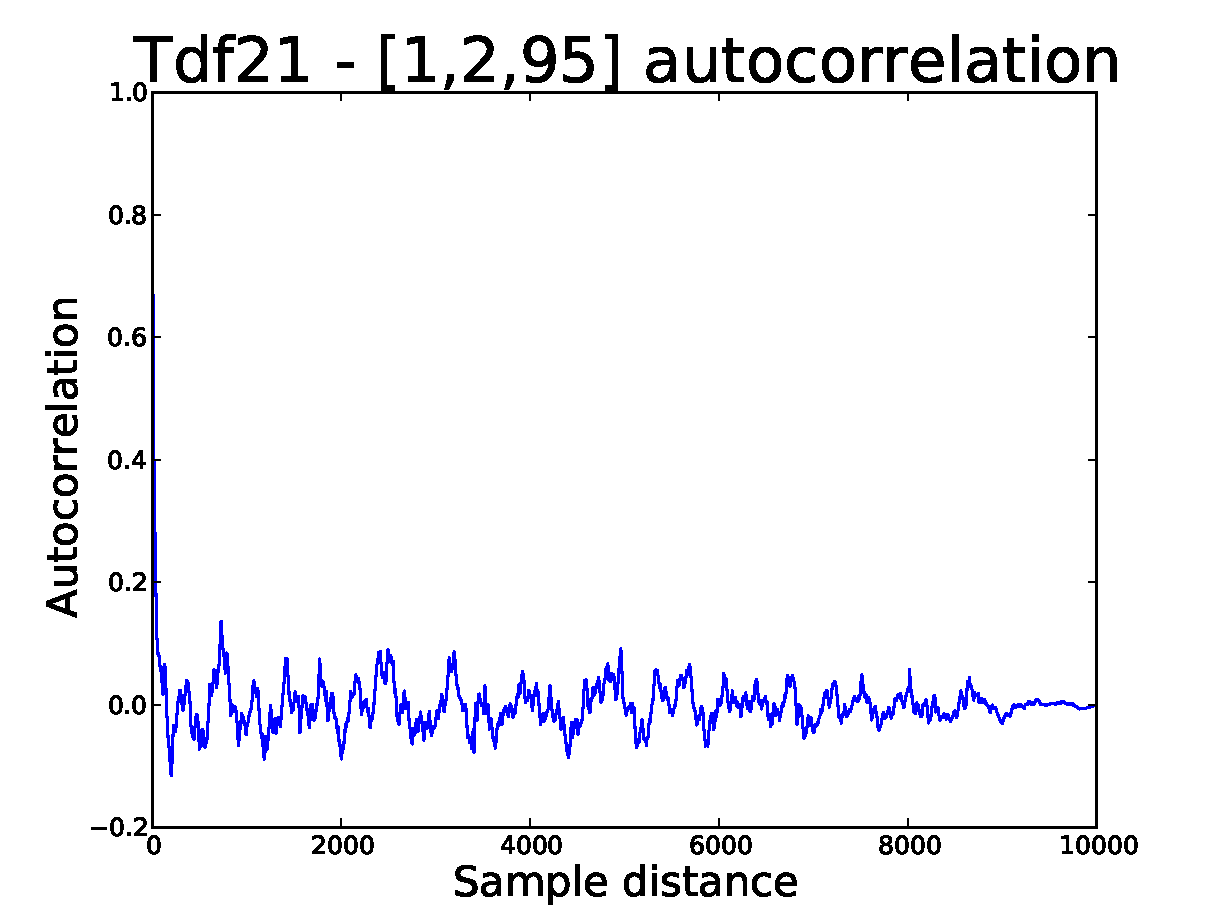
\includegraphics[width=\textwidth]{Tdf211295AutoCorr}
    \end{subfigure}
    \caption{Sample autocorrelations for the unpartitioned and the (1, 2, 95) partitioned priors, over 10,000 samples on the Tdf21 model.}
    \label{fig:tdf21PAutoCorr}
\end{figure}

Finally, Figure \ref{fig:tdf21PSampDist} shows the sample distributions. Here we can see that, despite the similar performance of the two priors on the mixing tests, the partitioned prior still results in a significantly smoother distribution.

\begin{figure}[h]
    \centering
    \begin{subfigure}[t]{0.48\textwidth}
      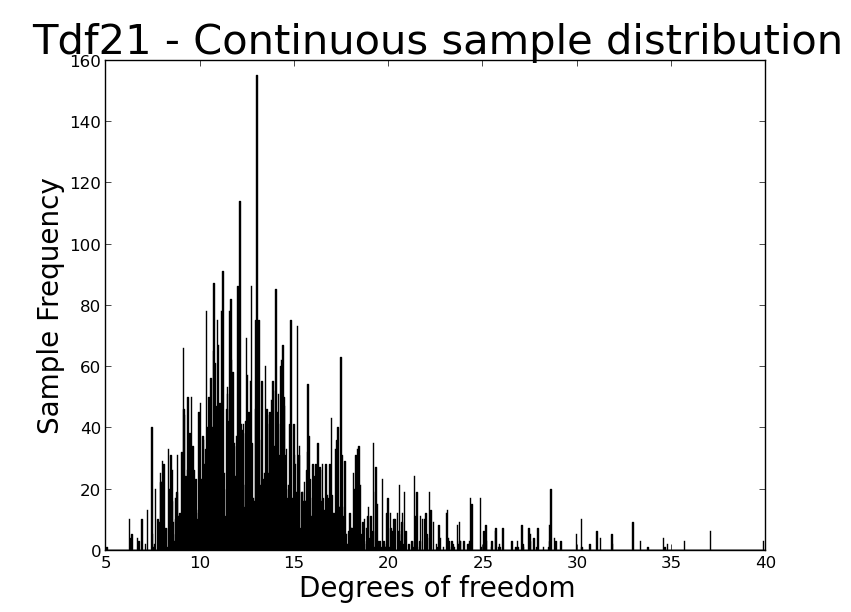
\includegraphics[width=\textwidth]{Tdf21SampDist}
    \end{subfigure}
    ~
    \begin{subfigure}[t]{0.48\textwidth}
      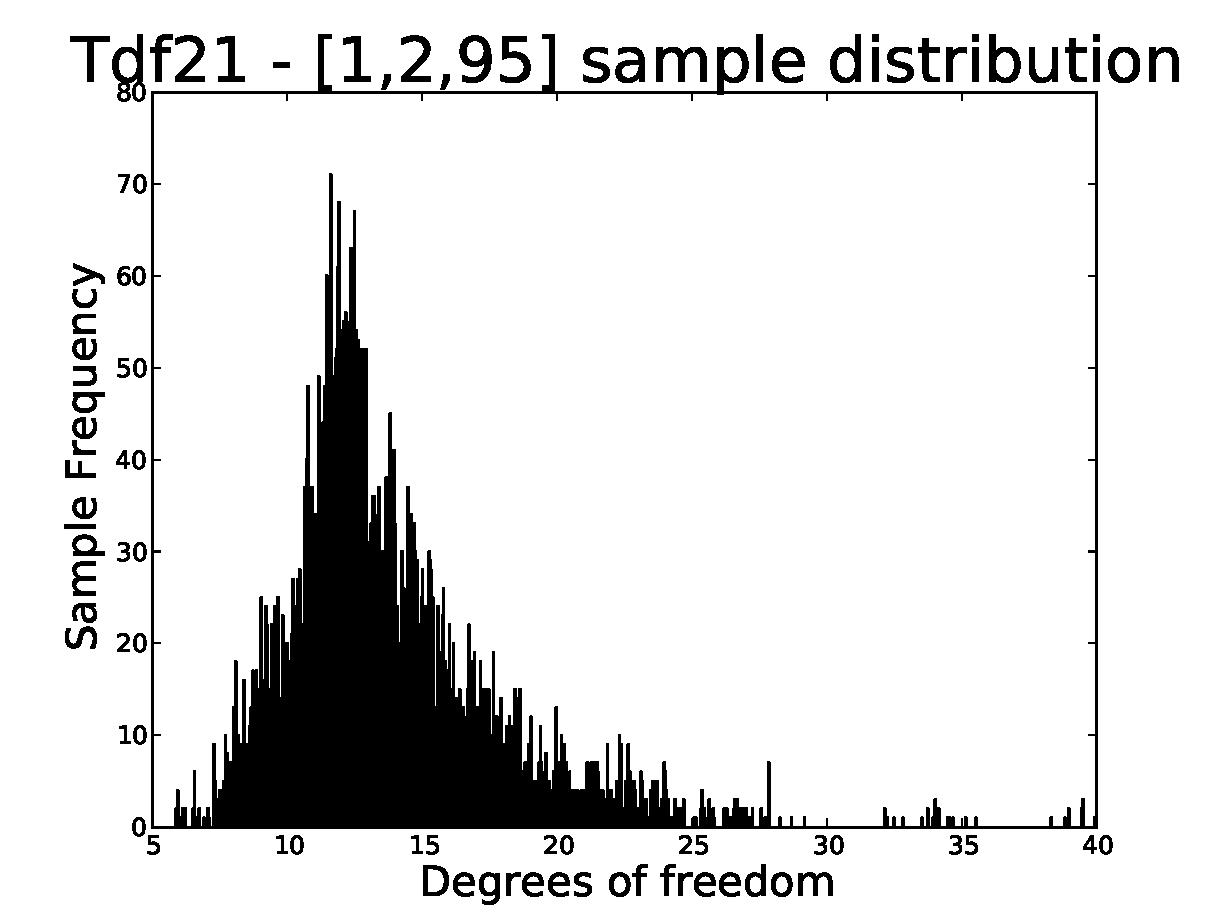
\includegraphics[width=\textwidth]{Tdf211295SampDist}
    \end{subfigure}
    \caption{Sample distributions for the unpartitioned and the (1, 2, 95) partitioned priors, over 10,000 samples on the Tdf21 model.}
    \label{fig:tdf21PSampDist}
\end{figure}

\section{Bit decomposition}
\label{sect:bitDecomp}
As mentioned in Section \ref{sect:sumUnif}, one problem with the sum of uniforms decomposition is that it alters the shape of a uniform prior. We would like to come up with decompositions that leave uniform priors invariant and that could therefore be applied indescriminately to re-write probabilistic programs containing such distributions. A family of invariant partitions of an uniform prior can be constructed by thinking in terms of the bit representation of the uniform samples. In order to be able to represent any real number, we can consider a bit representation of the number up to a certain precision and then add a single uniform-continuous value to the bit's value. 

\subsection{Definition}
In order to partition any uniform interval (uniform-continuous a b) it is sufficient to be able to partition the interval (uniform-continuous 0 1). Once this is accomplished, the target interval can be obtained through the transformation: (uniform-continuous a b) = a + (b-a) * (uniform-continuous 0 1).

In order to partition the interval (uniform-continuous 0 1) we first pick a bit depth, k, such that $ k \in \{ 0, 1, \ldots \infty \} $ We then define (uniform-continuous 0 1) $= flip*2^{-1} + flip*2^{-2} \ldots + flip*2^{-k} +$ (uniform-continuous 0 $2^{-k}$), where flip is a function which flips a coin and returns 0 or 1 with probability 1/2 each.

\subsection{Evaluation on Tdf and Tdf21}

To get an idea of the properties of bit decomposition we perform empirical evaluations on the Tdf and Tdf21 continuous models. Looking at the sample distributions in Figures \ref{fig:tdfPSampDist} and \ref{fig:tdf21PSampDist} we can see that a 3rd degree bit decomposition obtains similar performance to an unpartitioned prior. Intuitively this is because we are still subjecting proposals to the Metropolis-Hastings acceptance ratio, so if our program decides to flip one of the leading bits the proposal will be rejected, leading to bad mixing. As the depth of the bit decomposition increases, however, the probability that one of the leading bits is picked diminishes and therefore we will expect the mixing rate to improve. \todo{Should be possible to give some more formal results here.} We, however, restrict ourselves to a 3rd degree decomposition here since a higher degree variant would exhibit the problem ``stuck samples'', which is discussed in Section \ref{sect:stuckSamples}.

\begin{figure}[h]
    \centering
    \begin{subfigure}[t]{0.48\textwidth}
      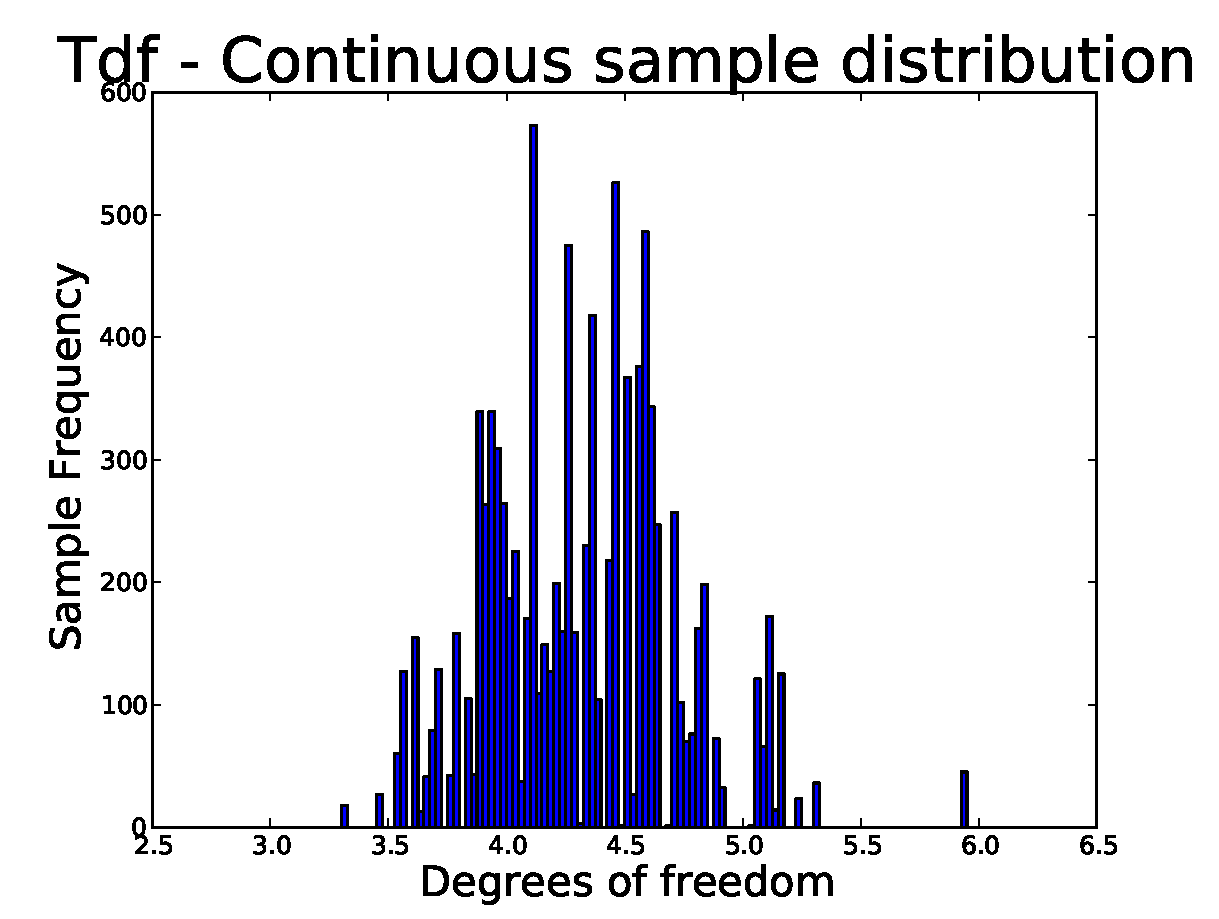
\includegraphics[width=\textwidth]{TdfSampDist}
    \end{subfigure}
    ~
    \begin{subfigure}[t]{0.48\textwidth}
      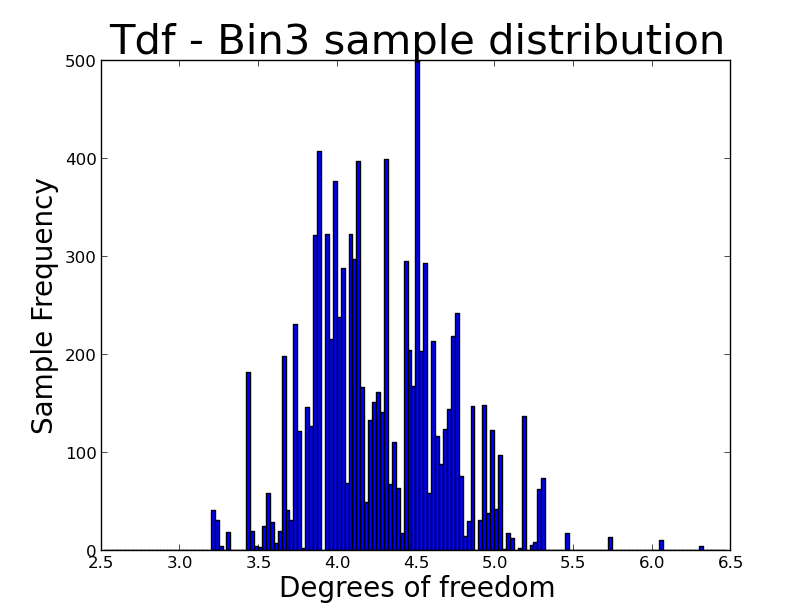
\includegraphics[width=\textwidth]{TdfBin3SampDist}
    \end{subfigure}
    \caption{Sample distributions for an unpartitioned and a 3 bit decomposition prior, over 10,000 samples on the Tdf continuous model.}
    \label{fig:tdfPSampDist}
\end{figure}

\begin{figure}[h]
    \centering
    \begin{subfigure}[t]{0.48\textwidth}
      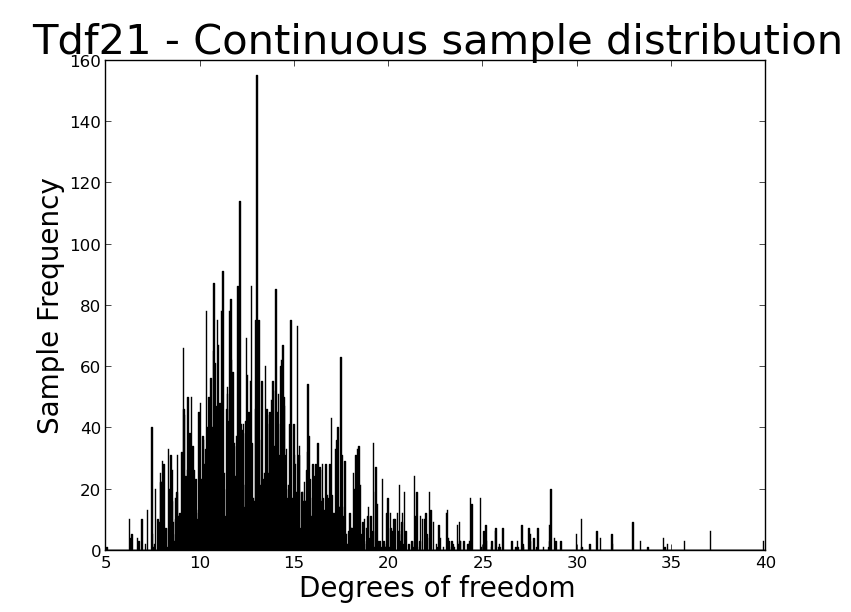
\includegraphics[width=\textwidth]{Tdf21SampDist}
    \end{subfigure}
    ~
    \begin{subfigure}[t]{0.48\textwidth}
      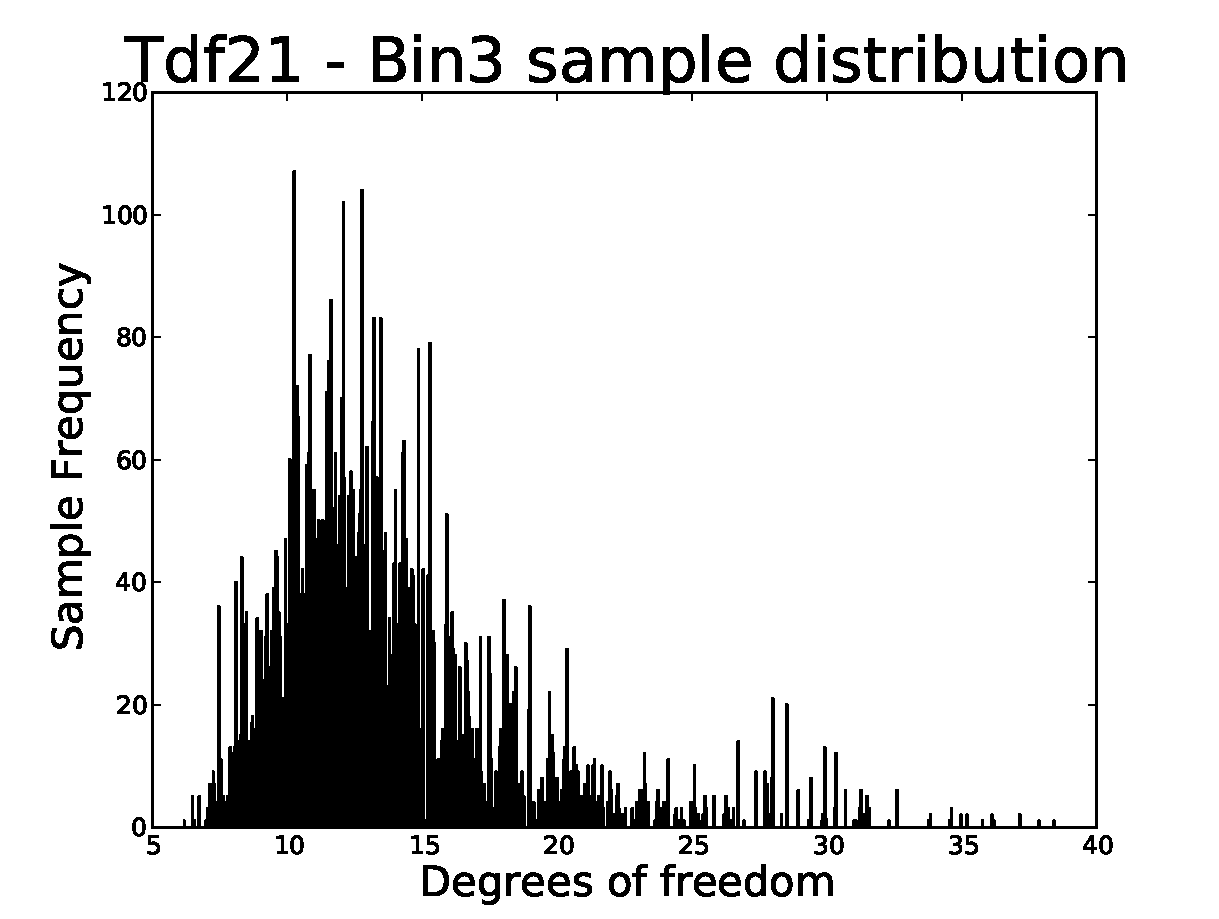
\includegraphics[width=\textwidth]{Tdf21Bin3SampDist}
    \end{subfigure}
    \caption{Sample distributions for an unpartitioned and a 3 bit decomposition prios, over 10,000 samples on the Tdf21 model.}
    \label{fig:tdf21PSampDist}
\end{figure}

The expected time to reach a mode neighbourhood is analyzed in Table \ref{tab:bestParts}. Here we can see that the 3rd degree binomial provides a significant improvement over the unpartitioned prior, though not as significant as the sum of uniforms does. \todo{talk about how binomials of different depth perform here}. On the depth 7 bit decomposition, we see good results on the small neighbourhoods but erratic ones on the larger neighbourhoods. The reason is again the fact that bit decompositions can result in ``stuck samples'', which are discussed in Section \ref{sect:stuckSamples}.

\begin{table}[H]
  \centering
  \begin{tabular}{llllll}
    \toprule
    \multirow{2}{*}{Model} & \multirow{2}{*}{Partition} & \multicolumn{4}{l}{Target neighbourhood size} \\
    \cmidrule(r){3-6} 
    & & 1 & 0.5 & 0.2 & 0.02 \\
    \midrule
    Both & Unpartitioned & 98 & 196 & 490 & 4900 \\
    \midrule
    \multirow{3}{*}{Tdf Continuous} & (1, 2, 95) & 130.06 & 155.48  & 186.83 & 317.31 \\
    & Bit 3 & 52 & 95.3  & 272.6 & 2232.4 \\
    & Bit 7 & 1080.78 & 866.64 & 776.26 & 1433.37 \\
    \midrule
    \multirow{3}{*}{Tdf21 Continuous} & (1, 2, 95) & 93.5 & 128.8  & 173.9 & 714.98 \\
    & Bit 3 & 117.52 & 170.65  & 401.5 & 2969.9 \\
    & Bit 7 & 161.86 & 177.22 & 284.99 & 1739.84 \\
    \bottomrule
  \end{tabular}
  \caption{Expected number of steps to neighbourhoods of the mode on the Tdf and Tdf21 continuous models for an unpartitioned prior, the (1,2,95) sum decomposition and 2 bit decompositions.}
  \label{tab:bestParts}
\end{table}

\subsection{Getting stuck on a bad sample}
\label{sect:stuckSamples}
A problem with the bit decomposition is that it is possible to construct scenarios in which a sample will get stuck and be arbitrarily unlikely to reach a particular neighbourhood of the mode. One simple such scenario can be constructed by assuming a guiding posterior log-likelihood that is convex, symmetric around the mode and steep enough that the probability of a sample moving significantly further away from the mode is negligible.

The simplest example of getting stuck can be observed by considering the bit decomposition of depth 1: (uniform-continuous 0 1) = $flip*2^{-1} +$ (uniform-continuous 0 $2^{-1}$). In this case, if the the mode is in the interval $[0.5 + \epsilon , 0.75]$, and $[mode - \epsilon, mode + \epsilon]$ is the mode neighbourhood we want to reach, then it is possible for the prior to get stuck outside of our target neighbourhood.
 
A concrete example would be:
\begin{flalign*}
  &\text{(uniform-continuous 0 1)} = flip*2^{-1} + \text{(uniform-continuous 0 }2^{-1})& \\
  &\quad\quad\quad\quad mode \sim 0.6 &\\
  &\quad\quad\quad\quad \epsilon \sim 0.05 &\\
  &\quad\quad\quad\quad flip \sim 0 &\\
  &\quad\quad\quad\quad \text{(uniform-continuous 0 }2^{-1}) \sim 0.4 &
\end{flalign*}

In this case, setting flip to $1$ would be very likely rejected since jumping from $0.4$ to $0.4 + 0.5 = 0.9$ takes us much further away from the mode at $0.6$ then we currently are. Further the uniform is likely to only accept resampled values in the $(0.4, 0.5)$ interval, which won't change the above situation. In order for us to get unstuck we would need either a very unlikely bit flip to be accepted or the uniform to accept a very unlikely resample close to 0, which could then be followed by a bit flip. Assuming we can make the log-likelihood arbitrarily steep around the mode, then we can expect to be stuck in this local optimum for an arbitrarily long number of samples.

Some possible solutions to avoid getting stuck would be:
\begin{itemize}

\item
Having the option of changing multiple bits at a time (eg: sample a variable to determine how many bits to change). This would ensure there are no hard local maximas. However, situations would still arise where a large number of bits would need to be concurrently changed to specific values in order for a sample to be accepted, which means we might still be stuck in a certain position for a long time untill just the right combination of bits is picked. \todo{is a more thorough analysis feasible here?}

\item
Using multiple shifted variants of the prior, where shifting by $shift$ means mapping sample $x$ to $(x + shift)\%1$). It can be shown that a single shift is enough to avoid getting stuck. However the effect on performance of adding shifts is complex, since performing a shift in an unstuck position can lead to us moving further away from the mode. More analysis of the effect of shifts is presented in \ref{sect:shifts}.

\item
Using multiple variants of the prior with different bit depths. If a sample is stuck on bit b, then moving it into a prior with depth < b will unstick it. However, this will result in the bits with the highest values being resampled more often, since they will be present in the most priors, which will have a negative effect on the mixing benefits offered by the decomposition. \todo{add more analysis on this}

\end{itemize}

One idea that is tempting but incorrect is to determine, with some likelihood, when a certain markov chain has become stuck based on its sample history. This would allow us to explicitly correct for the chain getting stuck. We could toss a coin to decide if we think we're currently stuck and if we decided we were not stuck we could sample normally. If we did think we were stuck, we could determine in which bits we might be stuck and pick one of these. We could then determine the interval in which the mode should be if we were indeed stuck on the bit we picked and sample uniformly from that interval.

This approach is atractive because, for the kth bit $flip*2^{-k}$, the target interval we would determine the mode to be in would be of size $2^{-k-1}$. However, the problem with this idea is that it isn't just picking proposals from a static prior or proposal kernel, but the proposal pattern is actually influenced by the sample history. This formulation would be conceptually similar to varying the width of our Metropolis-Hastings proposal kernel $Q(x_{new}|x_{old})$ based on the simulation history. However performing any such dynamic modification is not allowed if we wish to maintain the correct stationary distribution for our underlying Markov Chain \cite[p.~380]{mackay2003information}.

\subsection{Mixtures of shifted bit decompositions}
\label{sect:shifts}
In this section we explore two variants of the mixture of shifted bits. First we look at what is necessary simply to ensure that we'll never get stuck. Second we look at what is needed to be able to move from any stuck position to a neighbourhood of the mode in one jump. This second variant ends up providing better performance.

\subsubsection{Avoiding getting stuck}
\label{sect:stuckMath}
\todo{not sure if this section is clear enough. add diagrams?}

It turns out that a mixture of 2 bit decompositions, one of which is a shifted variant of the other, is sufficient to ensure that it is impossible to get stuck. However it seems we need to use a mixture of K priors in order to ensure that the binomial of depth K can move from any stuck position to the mode in one step. 

To better understand how these shifts work, we consider the formulation:
\begin{flalign*}
  &total = flip1*0.5 + flip2*0.25 + \text{(uniform-continuous 0 0.25)}& \\
  &\hspace{3em} flip1 \sim 0& \\
  &\hspace{3em} flip2 \sim 1& \\
  &\hspace{3em} \text{(uniform-continuous 0 0.25)} \sim \epsilon& \\
  &=> total = 0.25 + \epsilon \tag{$\epsilon$ is an arbitrarily small positive number}&
\end{flalign*}

Here we are stuck since, in order to reach the mode, we need to switch the $flip2$ bit to 0, but this flip will be rejected as it would mean moving significantly further away from the mode than we currently are. We want to determine what size of a shift needs to exist in order for us to be able to become unstuck. 

For any shift $s$ we choose, the shifted prior will be:
\[ shiftTotal = (s + total) \% 1 = (s + 0.25 + \epsilon) \% 1 \] 
And flipping the second bit ($flip2$) to 0 would result in a proposal:
\[proposal = s + \epsilon\]

We can now show that, if a shift is too small, then the proposal will be rejected. Specifically:
\begin{flalign*}
&\text{If } & \\
&\hspace{3em}mode = 0.25 - \epsilon &\\
&\hspace{3em} s < 0.125 - 2*\epsilon &\\
&\text{Then } & \\
&\hspace{3em} |shiftTotal - mode| = |s + 0.25 + \epsilon - 0.25 + \epsilon| = s + 2*\epsilon < 0.125 &\\
&\hspace{3em} |proposal - mode| = | s + \epsilon - 0.25 + \epsilon | = 0.25 - s + 2*\epsilon > 0.125 &\\
&=> distance(proposal, mode) > distance(shiftTotal, mode) \tag{which means the proposal is rejected}& 
\end{flalign*}

The only other proposals we could make is flipping the first bit ($flip1$) to 1 or increasing the uniform, both of which are also rejected since they move away from the mode in both shifts. Therefore, for the shift to be usefull on a stuck 2nd bit, we need that $s \geq 0.125$. Extrapolating, we see that in general, to get unstuck on the $k$th bit we require that $s \geq 2^{-k-1}$. Therefore it is sufficient to have one shift $s$ such that $s \geq 2^{-2}$ in order to guarantee that we never get stuck.

If, in addition to not getting stuck, we also want to be able to reach the mode in one jump from a stuck position, we must consider and additional example:
\begin{flalign*} 
& total = flip1*0.5 + flip2*0.25 + \text{(uniform-continuous 0 0.25)} &\\ 
& \hspace{3em} flip1 \sim 0 &\\ 
& \hspace{3em} flip2 \sim 0 &\\ 
& \hspace{3em} \text{(uniform-continuous 0 0.25)} \sim 0.25 - \epsilon &\\ 
& => total = 0.25 - \epsilon \tag{$\epsilon$ is an arbitrarily small positive number}&
\end{flalign*}

As before, for any shift $s$ we choose, the shifted prior will be:
\[shiftTotal = (s + total) \% 1 = (s + 0.25 - \epsilon) \% 1\]
And the only proposal that decreases the sample size is from reducing the uniform-continuous variable. Therefore
\[proposal \geq s + \epsilon\]

We can now show that a shift that is too large fails to satisfy our criteria. Specifically:
\begin{flalign*}
&\text{If } & \\
&\hspace{3em} mode = 0.25 + \epsilon &\\
&\hspace{3em} s > 0.25 + 2*\epsilon &\\
&\text{Then } & \\
&\hspace{3em} |shiftTotal - mode| = |s + 0.25 - \epsilon - 0.25 - \epsilon| = s - 2*\epsilon > 0.25 &\\
&\hspace{3em} |proposal - mode| \geq s + \epsilon - 0.25 - \epsilon > \epsilon &\\
&=> distance(proposal, mode) > \epsilon \tag{which means we can't reach the mode in 1 step}& 
\end{flalign*}

The only other proposals possible in this situation are to shift one of the bits to 1, which would just take us farther from the mode. In the above scenario, it is therefore impossible to reach the mode by performing a shift and a proposal.

Note that, in this situation we are not stuck. For instance, if we accept $\text{(uniform-continuous 0 0.25)} = \epsilon$ we will have $shiftTotal > mode + \epsilon$. If we then switch back to the original $0 shift$ we obtain in $total = mode + \epsilon - s = mode + \epsilon - s$. And since $s > 0.25 + 2*\epsilon$ we would now have $total < mode - 0.25 - \epsilon$ and we would therefore be in a position to accept switching the 2nd bit to 1, which would unstick us.

However, if we wish to jump to the mode from a postiion stuck on the second bit, we've shown that the shift must have the property:
\[0.125 <= s <= 0.25\]
And in general, to guarantee that we can jump to the mode when stuck on the $k$th bit, we need to have a shift $s$ such that:
\[2^{-k-1} <= s <= 2^{-k}\]
This implies that we need a different sized shift for every bit.

\subsubsection{Empirical performance}

The arguments in the previous section suggest that the placement of the mode can significantly affect the likelihood of getting stuck. In order to get a better idea of the effect of the mode location we test the burn-in time for different mode placements. First we look at burn-in time averaged over all mode placements $m$, where $m \in [0.0005, 0.0015,…, 0.9995]$ and $\epsilon = 0.0005$.

In \ref{fig:allMaxShifts} we look at the case where we resample the shift on each iteration and we have shifts of size $2^{-k}$ (called maximum shifts) for each bit position k. Here the unpartitioned prior corresponds to the bit decomposition of depth 0. While the improvements in burn-in rate are not as significant when averaging over all mode placements as they were for our initial experiments on the Tdf models, a 2x speed-up can still be obtained.

\begin{figure}[h]
    \centering
    \begin{subfigure}[t]{0.48\textwidth}
      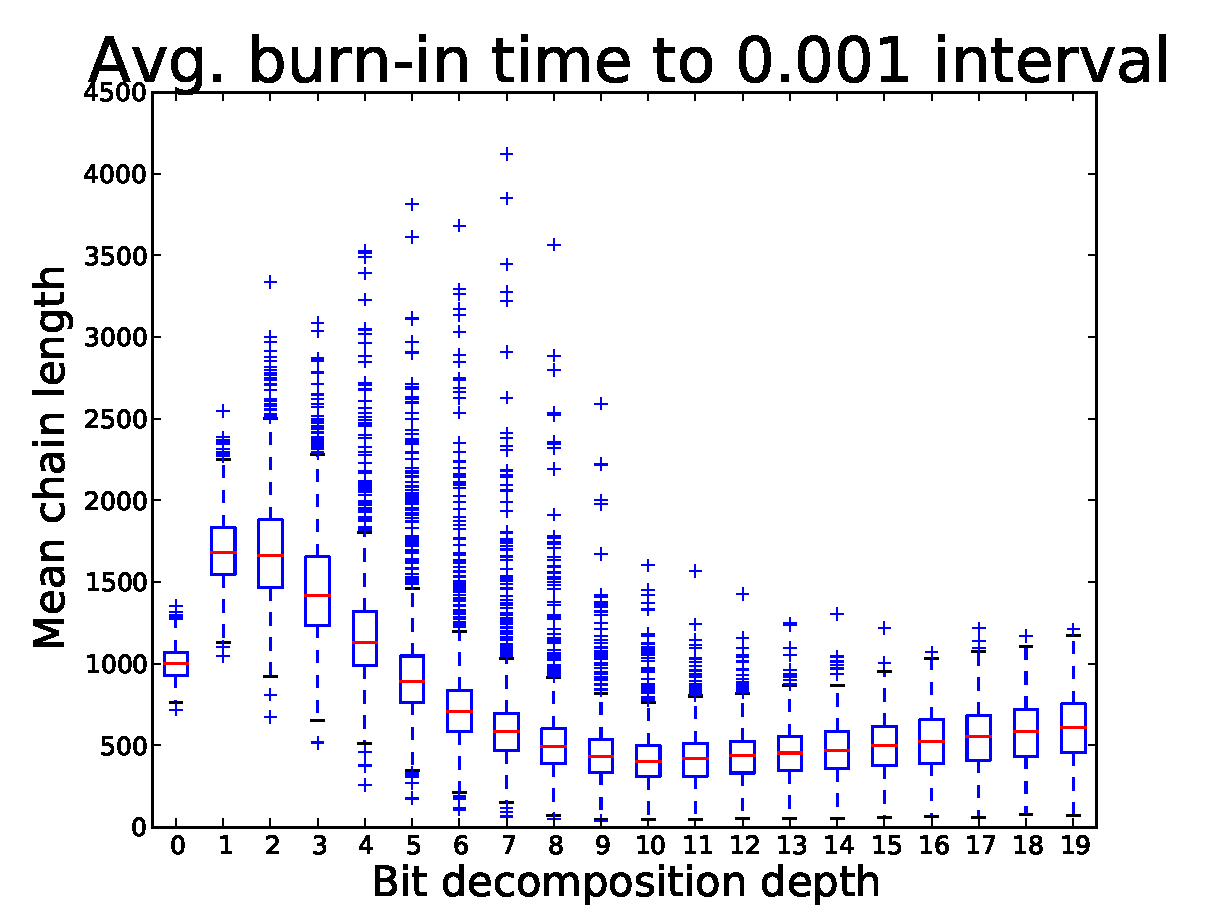
\includegraphics[width=\textwidth]{AllShiftsMax0001}
      \caption{Maximum sized shifts.}
      \label{fig:allMaxShifts}
    \end{subfigure}
    ~
    \begin{subfigure}[t]{0.48\textwidth}
      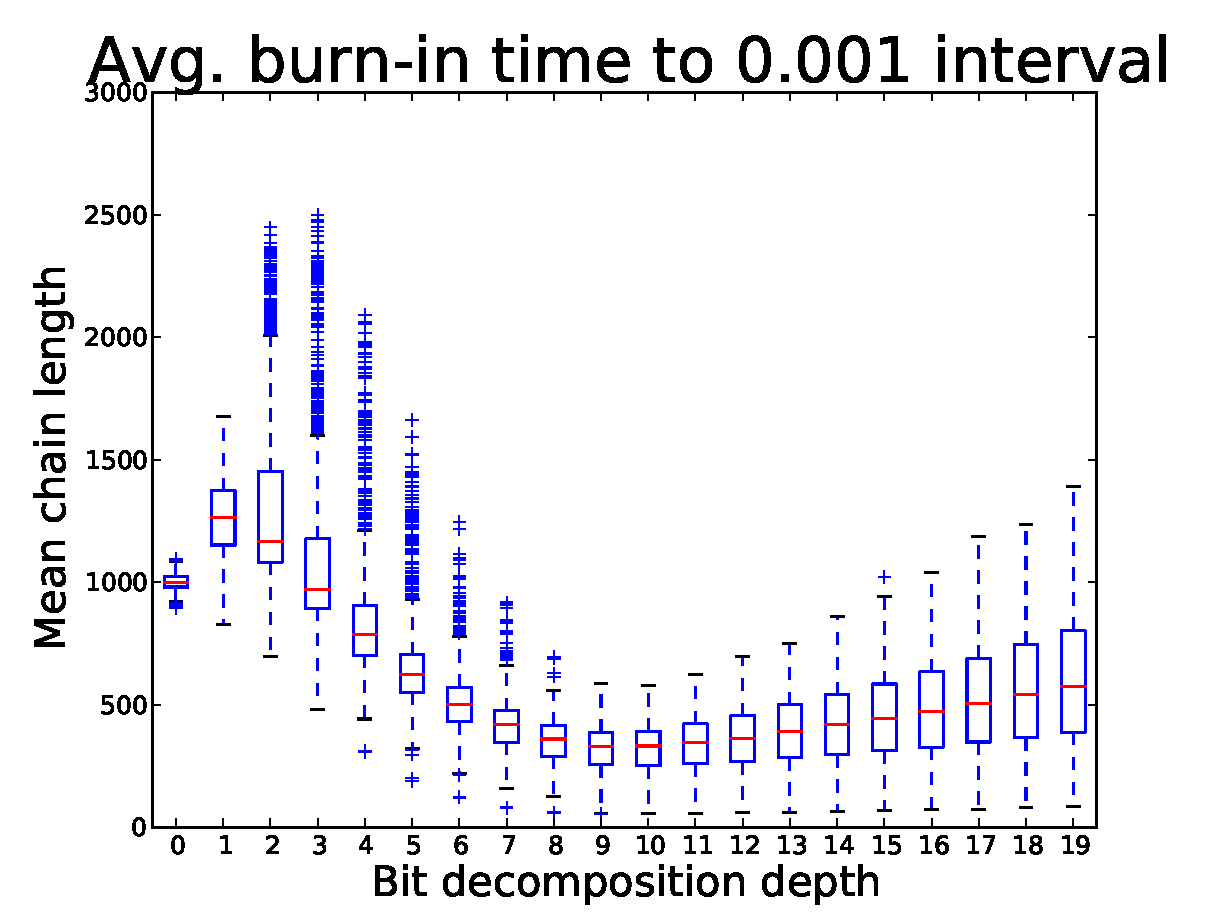
\includegraphics[width=\textwidth]{AllShiftsMin0001}
      \caption{Minimum sized shifts.}
      \label{fig:allMinShifts}
    \end{subfigure}
    \caption{Time to 0.001 neighbourhood of mode, averaged over all mode placements, for bit decompositions of different depths using a shift for every bit.}
    \label{fig:allShifts}
\end{figure}


As explained in Section \ref{sect:stuckMath}, the shift size $s$ for bit $k$ needs to respect $2^{-k-1} <= s <= 2^{-k}$ in order for us to be able to jump to the mode in one step. In \ref{fig:allMinShifts} we check whether the choice of shift size within this interval is significant, by looking at the burn-in rate for shifts of size $2^{-k-1}$ (called minimum shifts) for each bit position k. The results are quite similar to those obtained for the maximum shifts, which suggests that the performance isn't sensitive to the choice of shift length within $[2^{-k-1}, 2^{-k}]$.

We would also like to see what happens as the size of the target neighbourhood changes. In Figure \ref{fig:AllShiftsMax001} we repeat the max shift experiment for a target neighbourhood of size 0.01 (10x larger). While the bit decomposition still gives some advantage, as the size of the target neighbourhood increases this advantage appears to become less significant. Intuitively this happens because a larger number of the less significant bits become irrelevant as far as ending up in the desired region is concerned.

\begin{figure}[h]
    \centering
    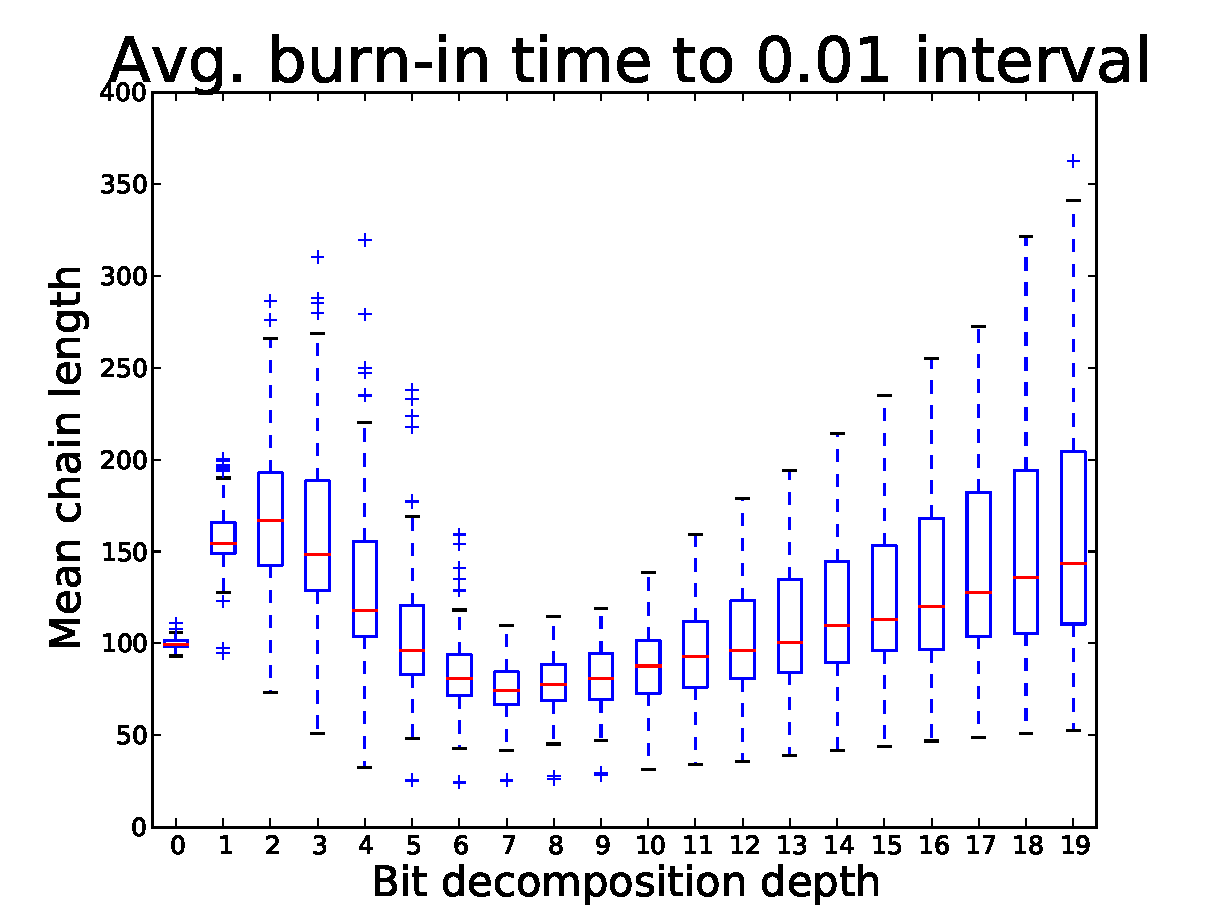
\includegraphics[width=0.8\textwidth]{AllShiftsMax001}
    \caption{Time to 0.01 neighbourhood of mode, averaged over all mode placements, for bit decompositions of different depths using a shift for every bit.}
    \label{fig:AllShiftsMax001}
\end{figure}

Finally, we would also like to see what happens to the performance if we do not provide k shifts for k bits, but instead only 1 or 2 shifts. As explained in section \ref{sect:stuckMath}, a single properly sized shift is sufficient to stop us from getting stuck. However, without k shifts for k bits, we sacrifice the ability of always moving from a stuck position to the mode in one step. As seen in Figure \ref{fig:fewShifts}, this seems to have a significant negative effect on the decompositions' performance. \todo{talk about distributions over shifts, and more about benefits/drawback of shifts and/or changing depths}

\begin{figure}[h]
    \centering
    \begin{subfigure}[t]{0.48\textwidth}
      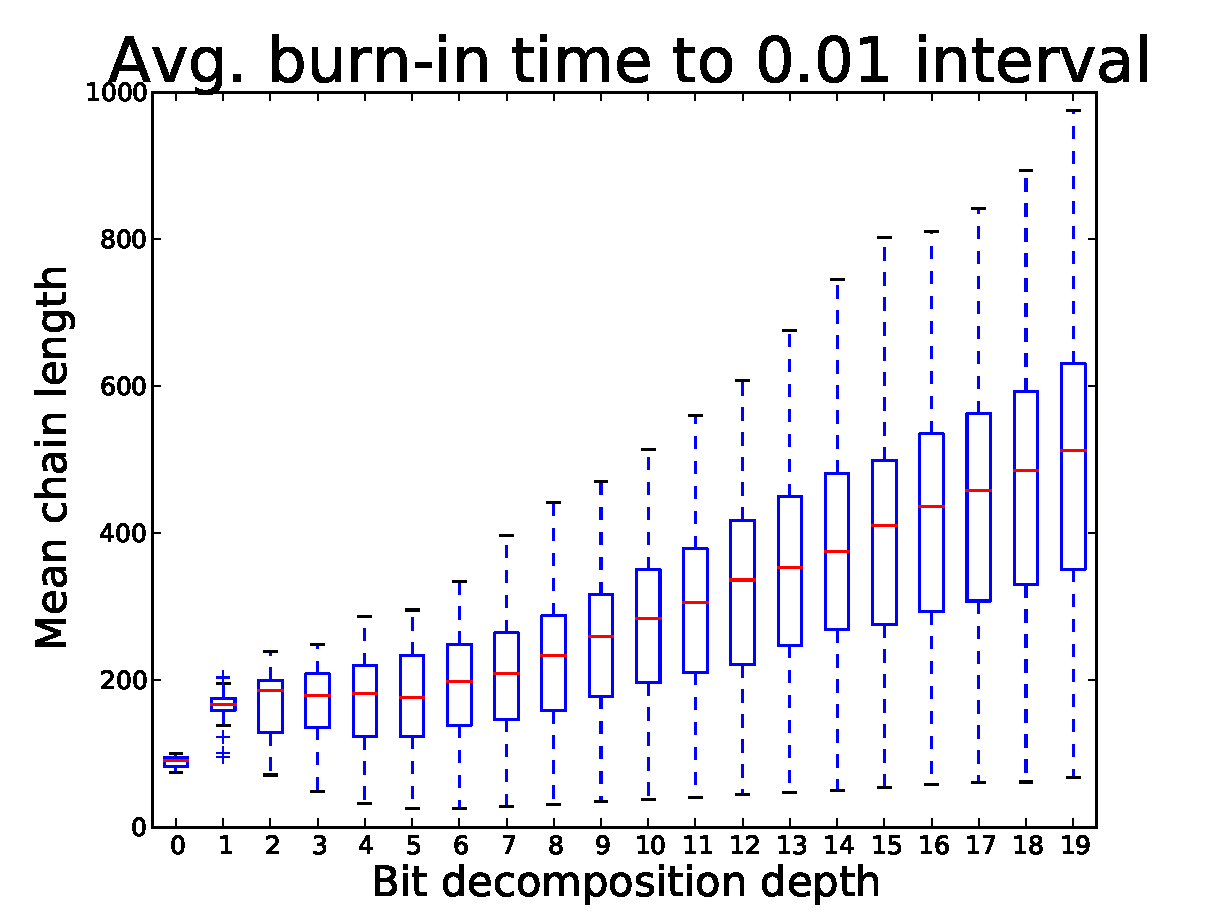
\includegraphics[width=\textwidth]{05Shift001}
      \caption{Shift of size 0.5}
    \end{subfigure}
    ~
    \begin{subfigure}[t]{0.48\textwidth}
      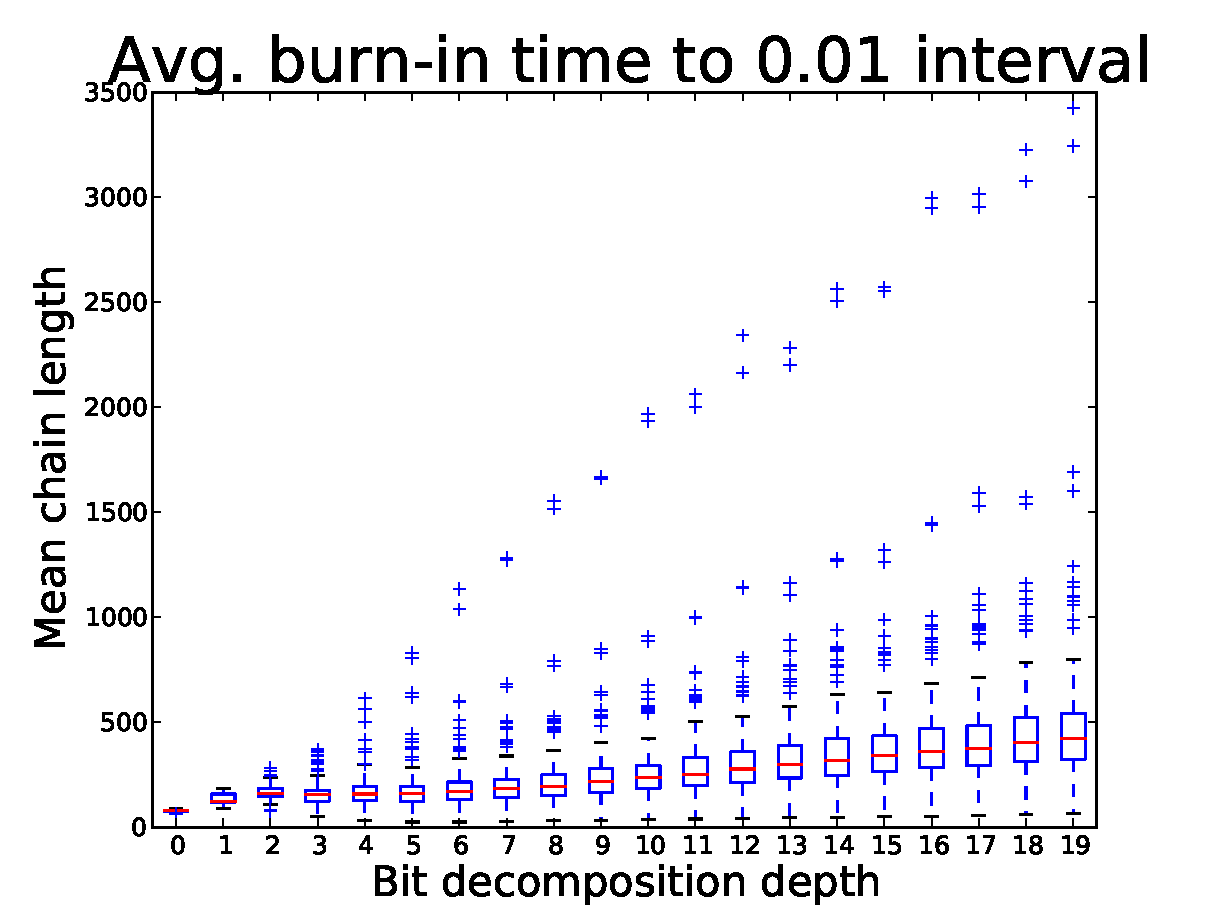
\includegraphics[width=\textwidth]{02505Shift001}
      \caption{Shift of size 0.25 and 0.5}
    \end{subfigure}
    \caption{Time to 0.01 neighbourhood of mode, averaged over all mode placements, for bit decompositions of different depth using a small number of shifts.}
    \label{fig:fewShifts}
\end{figure}

\subsubsection{Determining optimal shifts and shift transitions}
It seems we have a wide variety of options regarding what shifts to use and how to transition between them. It therefore seems worthwhile to consider the question of whether we can determine any optimal solutions analytically. 

In order to do so, we make some observations:
\begin{itemize}

\item
The location of the mode neighbourhood determines which regions are traps (i.e. in which regions, once you enter, you can no longer reach the mode without shifting)

\item
The current sample determines what portion of the traps (if any) are still accessible (based on the assumption that it is arbitrarily unlikely for the log-likelihood to decrease between consecutive samples).

\item
The probability of getting to the mode or falling in a trap cannot be modelled with (mixtures of) geometric distributions since a sample's probability distribution depends on the previous samples (and is therefore not uniform, unless we integrate out its history)

\item
For a set mode and log-likelihood function we can represent the transition between samples via a bit-level markov chain which ignores the trailing uniform. We can then create absorbing states representing the mode neighbourhood and the traps.

\item
If, for instance, the neighbourhood is only 0.1 of the length of the smallest bit we would implicitly represent the uniform only in the corresponding bit state by giving a 0.1 transition from this bit state to the mode-neighbourhood absorbing state. This however ignores the movement of the uniform during normal sampling which may end up biasing the results since, for instance, if the mode is in the leftmost bit the uniform will likely already have a very small value by the time the correct bit state is reached. \todo{There seem to be heuristic ways to address this}

\item
Using this formulation we can analytically derive the probability of getting stuck and the expected number of steps to the mode. Representing shifted priors is also possible. The simplest way would be to have 2x the nodes for a combination of 2 shifted priors.

\end{itemize}
\todo{try to get some results using markov chain implementation. Otherwise there's not much point in describing it ...}



\chapter{Novel PPL inference techniques}
\label{chap:infEngines}

In the previous chapter we attempted to re-write probabilistic programs in such a way as to improve the performance of local, single-site, Metropolis-Hastings inference. However this approach may prove limiting, so we are also interested in exploring different inference techniques that may perform better, at least on some subset of possible models. In this chapter we explore one such technique, slice sampling, while also briefly looking at some issues of tangential interest.

\section{Preliminaries}
In order to implement a PPL based on a new inference technique we need to understand both how the inference technique in question works and how we may build a PPL in general.

\subsection{Slice sampling}
\label{sect:sliceBack}
\todo{add basic description of slice sampling}

\subsection{Basic PPL Construction}
\todo{add basic description of lightweight style PPL construction}

\section{Stochastic Python}
\label{sect:StocPy}
\todo{add description of implementation, space permitting}

\section{Slice sampling inference engine}
\subsection{Custom Slice Sampling and Metropolis on Tdf models}

As a preliminary test, we implement custom slice sampling and local metropolis-hastings algorithms for the Tdf continuous and Tdf21 continuous models. A comparison of the burn-in needed to reach a neighbourhood of the mode is presented in Figure \ref{fig:SliceMetCustPerf}. Slice sampling has a much shorter burn-in on these models. In fact slice sampling does better than any of the partitioned priors did (averaged over the all posterior mode placements).

\begin{figure}[h]
    \centering
    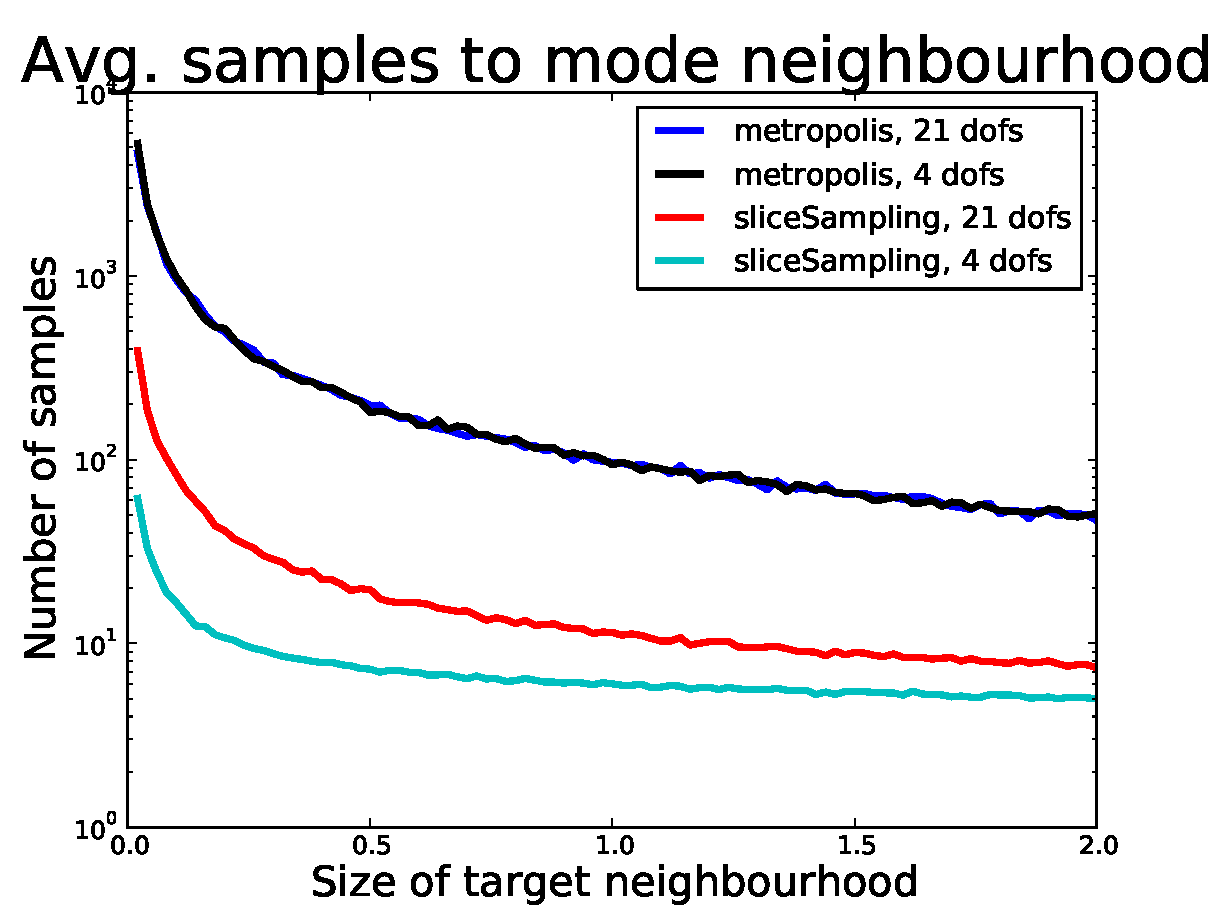
\includegraphics[width=0.8\textwidth]{SliceMetCustPerf}
    \caption{Burn-in time for local metropolis-hastings and slice sampling, on the two continuous Tdf models, as the target neighbourhood varies.}
    \label{fig:SliceMetCustPerf}
\end{figure}

However the performance of slice sampling does seem to vary with the shape of the likelihood. In Figure \ref{fig:sliceGaussLik} we investigate this behaviour by modeling the likelihood as a Gaussian and seeing how slice performs as we vary the Gaussian's properties.

\begin{figure}[h]
    \centering
    \begin{subfigure}[t]{0.48\textwidth}
      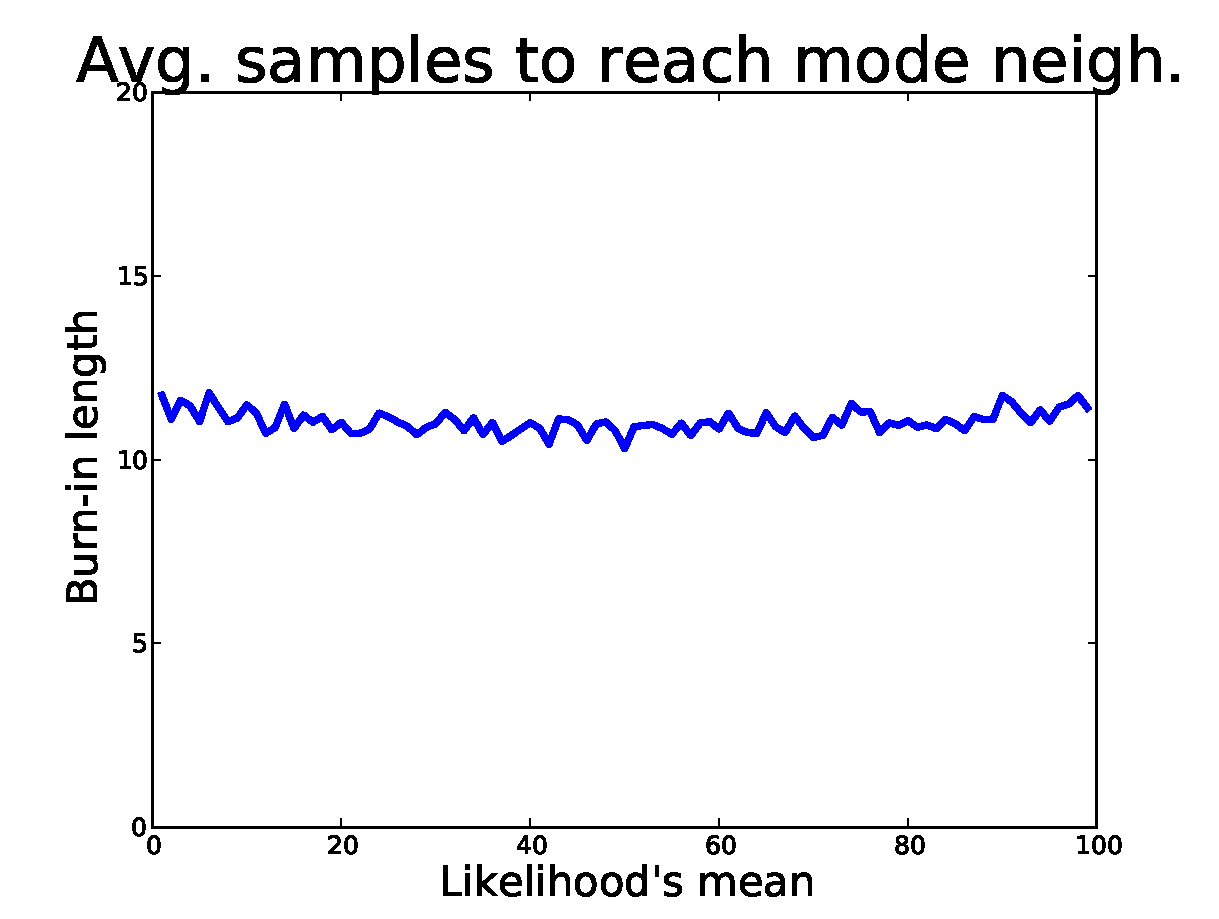
\includegraphics[width=\textwidth]{SliceSampsMean}
      \caption{Effect of likelihood mean}
    \end{subfigure}
    ~
    \begin{subfigure}[t]{0.48\textwidth}
      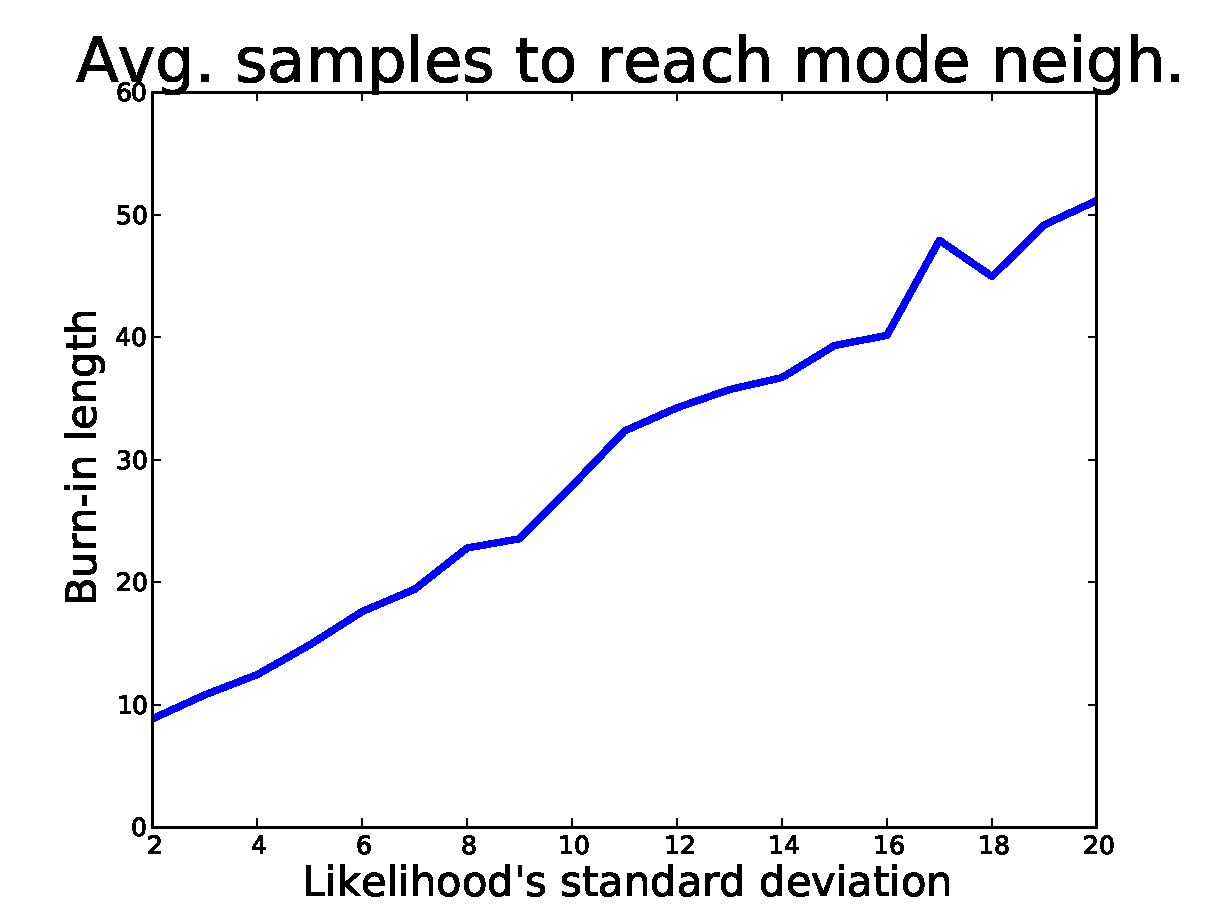
\includegraphics[width=\textwidth]{SliceSampsStd}
      \caption{Effect of likelihood standard deviation}
    \end{subfigure}
    \caption{Average burn-in time for slice sampling guided by a Gaussian likelihood of varying mean and standard deviation}
    \label{fig:sliceGaussLik}
\end{figure}

It seems that the placement of the likelihood in the interval doesn't affect performance, but the width of the distribution does. For reference, the Gaussian likelihoods with minimum and maximum standard deviations that we tested are shown in Figure \ref{fig:gaussStdDev}.

\begin{figure}[h]
    \centering
    \begin{subfigure}[t]{0.48\textwidth}
      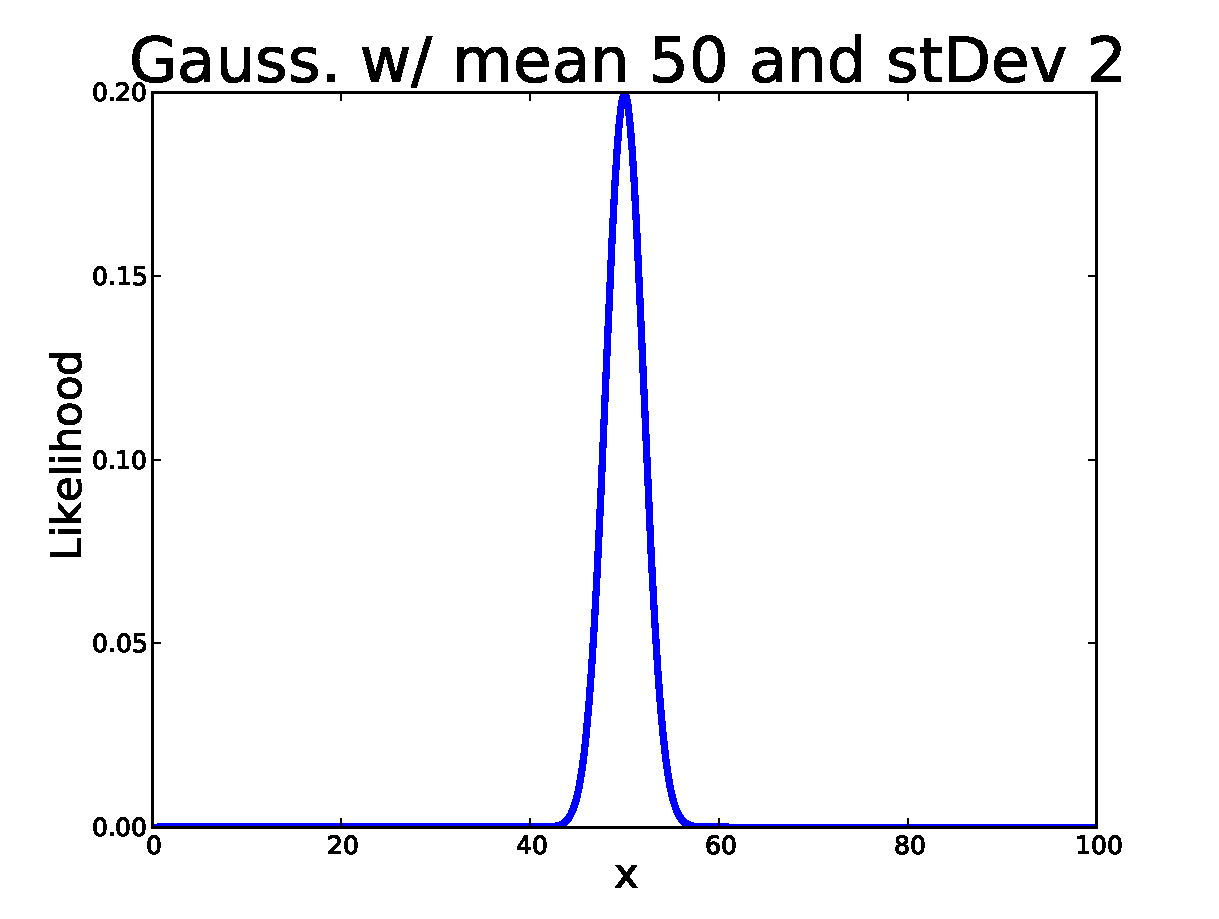
\includegraphics[width=\textwidth]{Gauss2}
    \end{subfigure}
    ~
    \begin{subfigure}[t]{0.48\textwidth}
      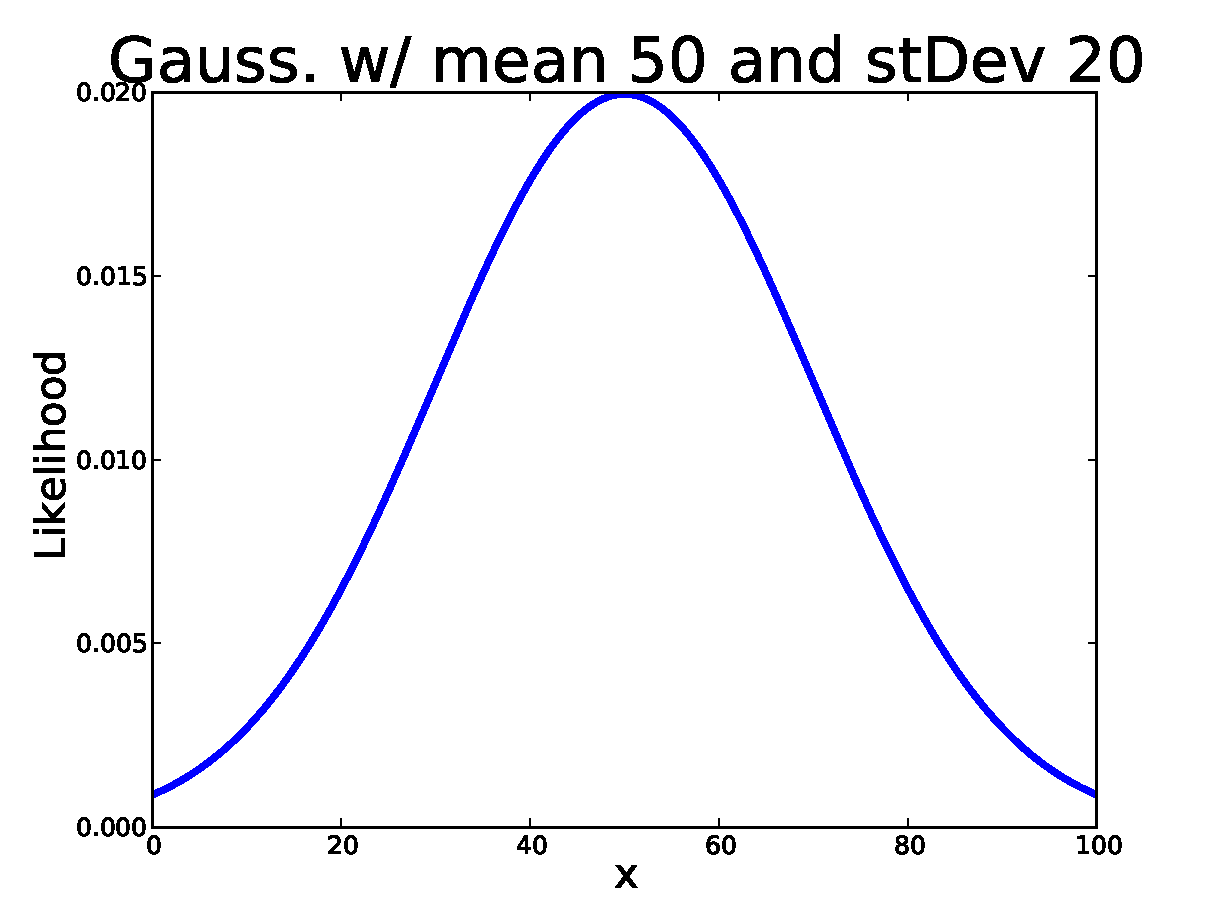
\includegraphics[width=\textwidth]{Gauss20}
    \end{subfigure}
    \caption{The smallest and largest Gaussian standard deviation considered in Figure \ref{fig:sliceGaussLik}}
    \label{fig:gaussStdDev}
\end{figure}

Next, we examine the mixing properties of local metropolis-hastings and slice sampling by considering the sample evolution (Figure \ref{fig:custSampEvol}), the sample autocorelation (Figure \ref{fig:custAutoCorr}) and the empirical distributions (Figure \ref{fig:custSampDist}) obtained by the two methods. For the obtained distributions to be comparable, we keep the number of log-likelihood computations performed by the two methods equal. This means that, while metropolis-hastings is allowed 10,000 samples, we only take 1962 from slice sampling (since, on this model, slice sampling averages just over 5 likelihood computations per extracted sample).

\begin{figure}[h]
    \centering
    \begin{subfigure}[t]{0.48\textwidth}
      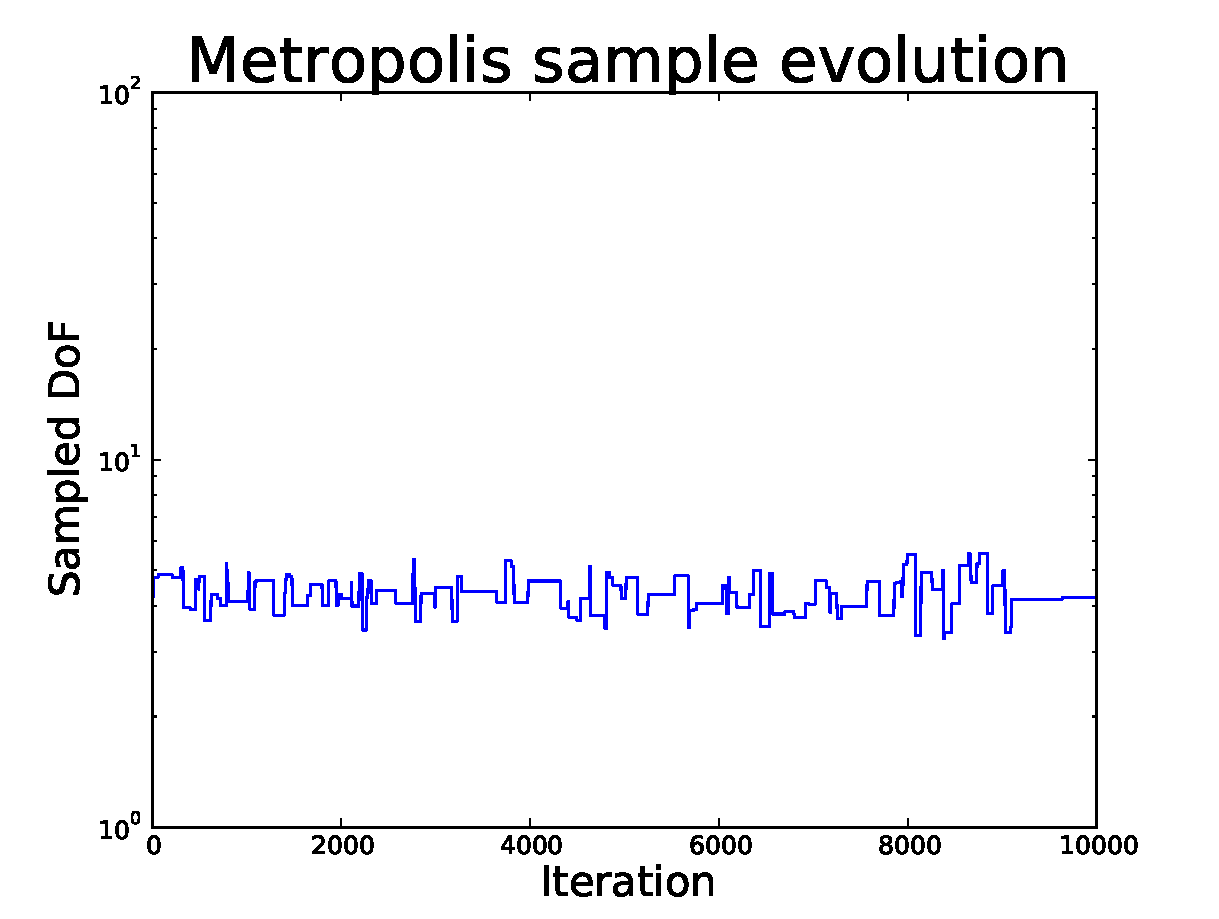
\includegraphics[width=\textwidth]{MetSampEvol}
    \end{subfigure}
    ~
    \begin{subfigure}[t]{0.48\textwidth}
      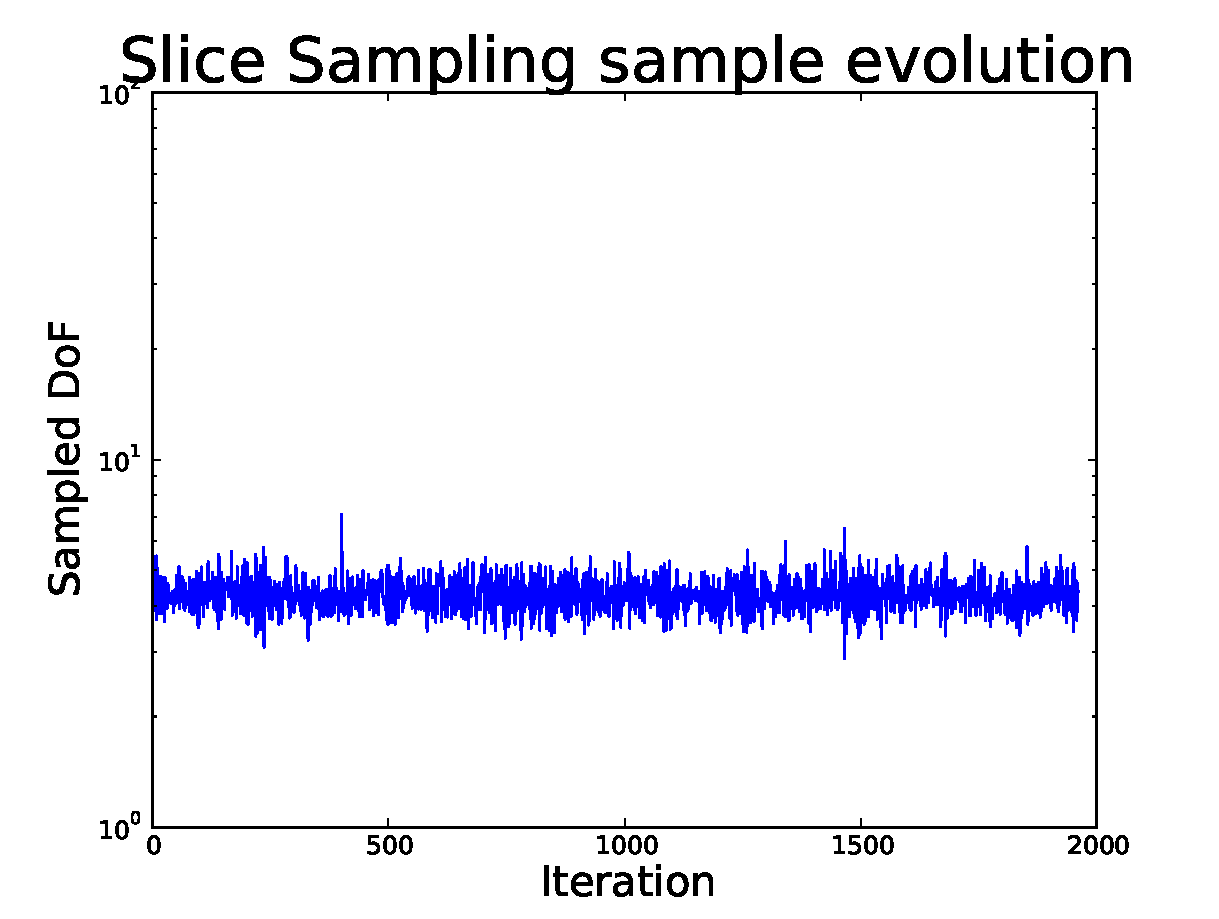
\includegraphics[width=\textwidth]{SliceSampEvol}
    \end{subfigure}
    \caption{Sample evolution of local metropolis and slice sampling on the Tdf continuous model}
    \label{fig:custSampEvol}
\end{figure}

\begin{figure}[h]
    \centering
    \begin{subfigure}[t]{0.48\textwidth}
      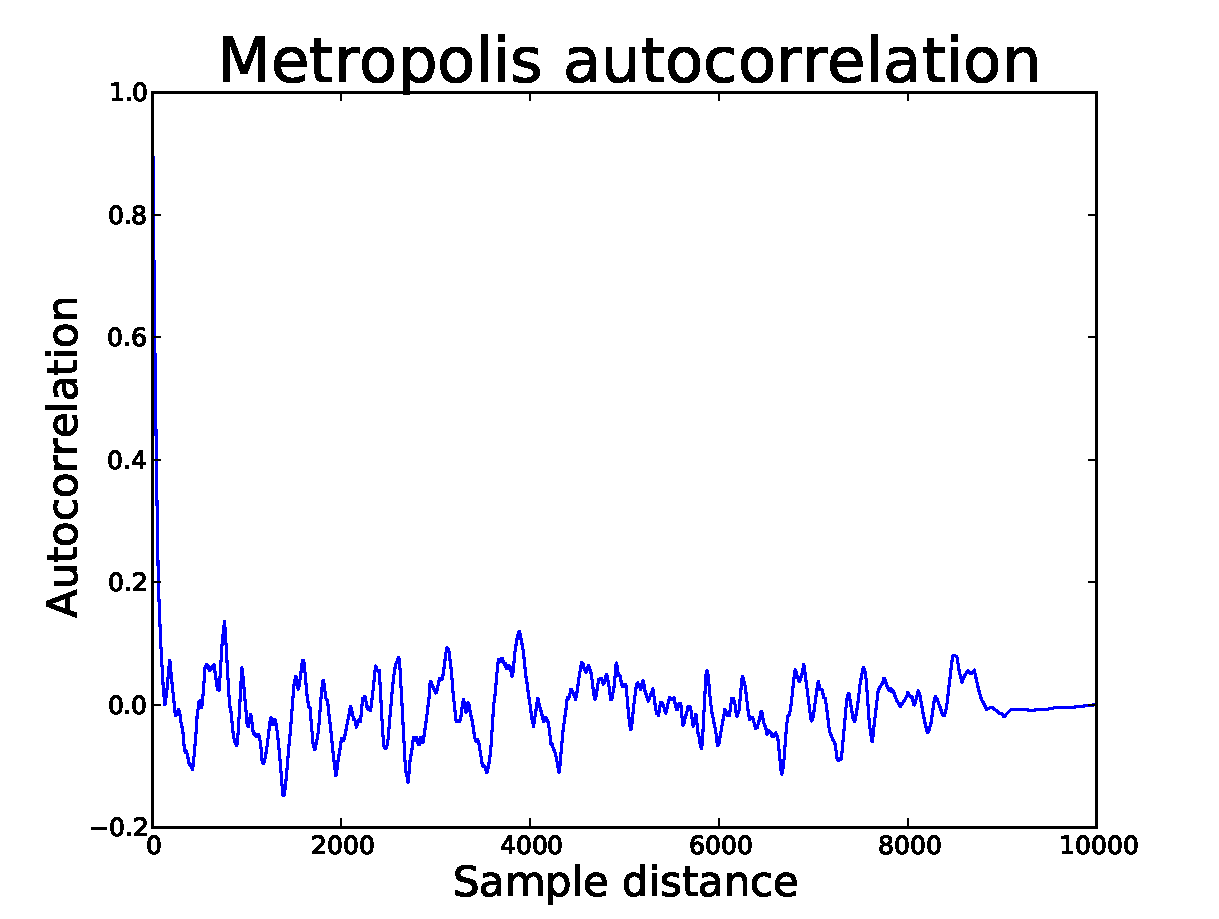
\includegraphics[width=\textwidth]{MetAutoCorr}
    \end{subfigure}
    ~
    \begin{subfigure}[t]{0.48\textwidth}
      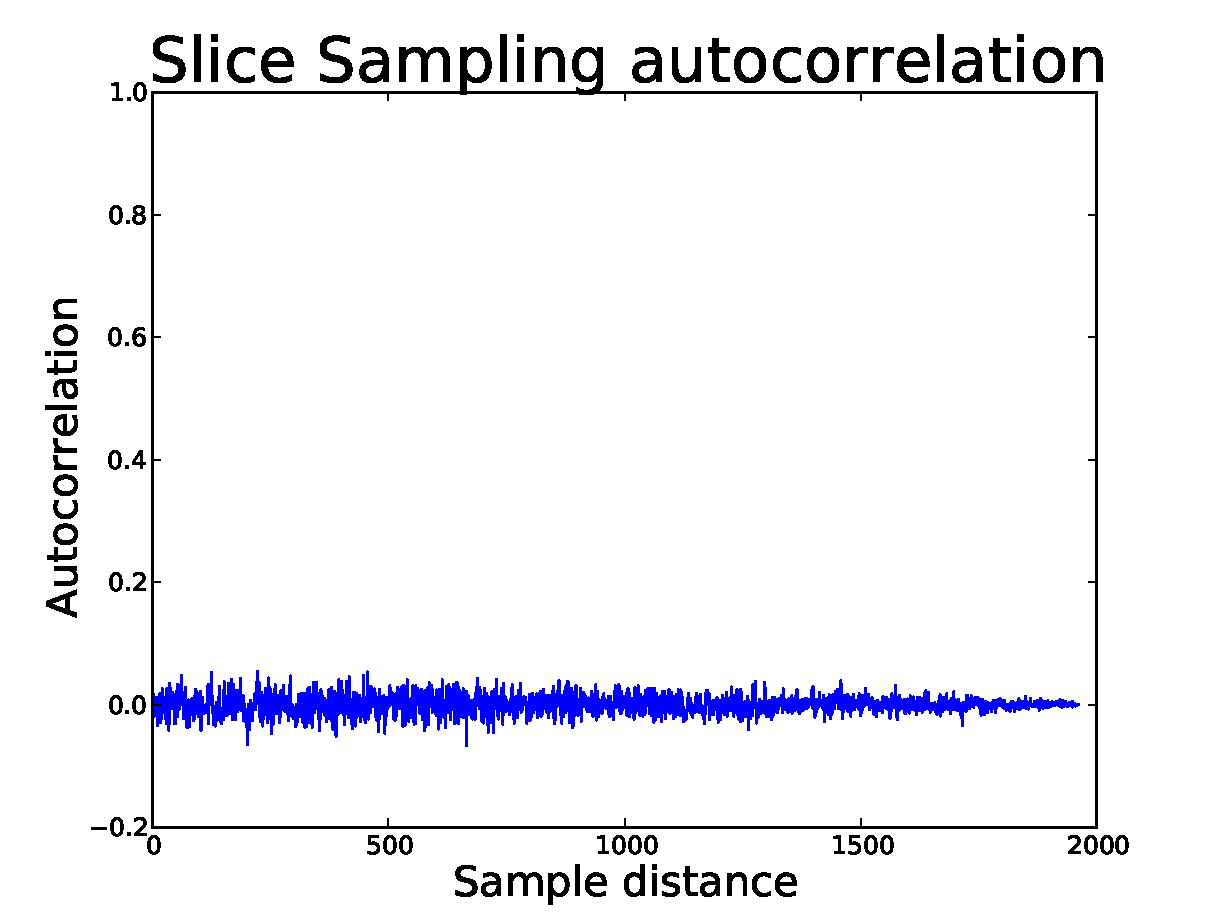
\includegraphics[width=\textwidth]{SliceAutoCorr}
    \end{subfigure}
    \caption{Sample autocorrelation of local metropolis and slice sampling on the Tdf continuous model}
    \label{fig:custAutoCorr}
\end{figure}

\begin{figure}[H]
    \centering
    \begin{subfigure}[t]{0.48\textwidth}
      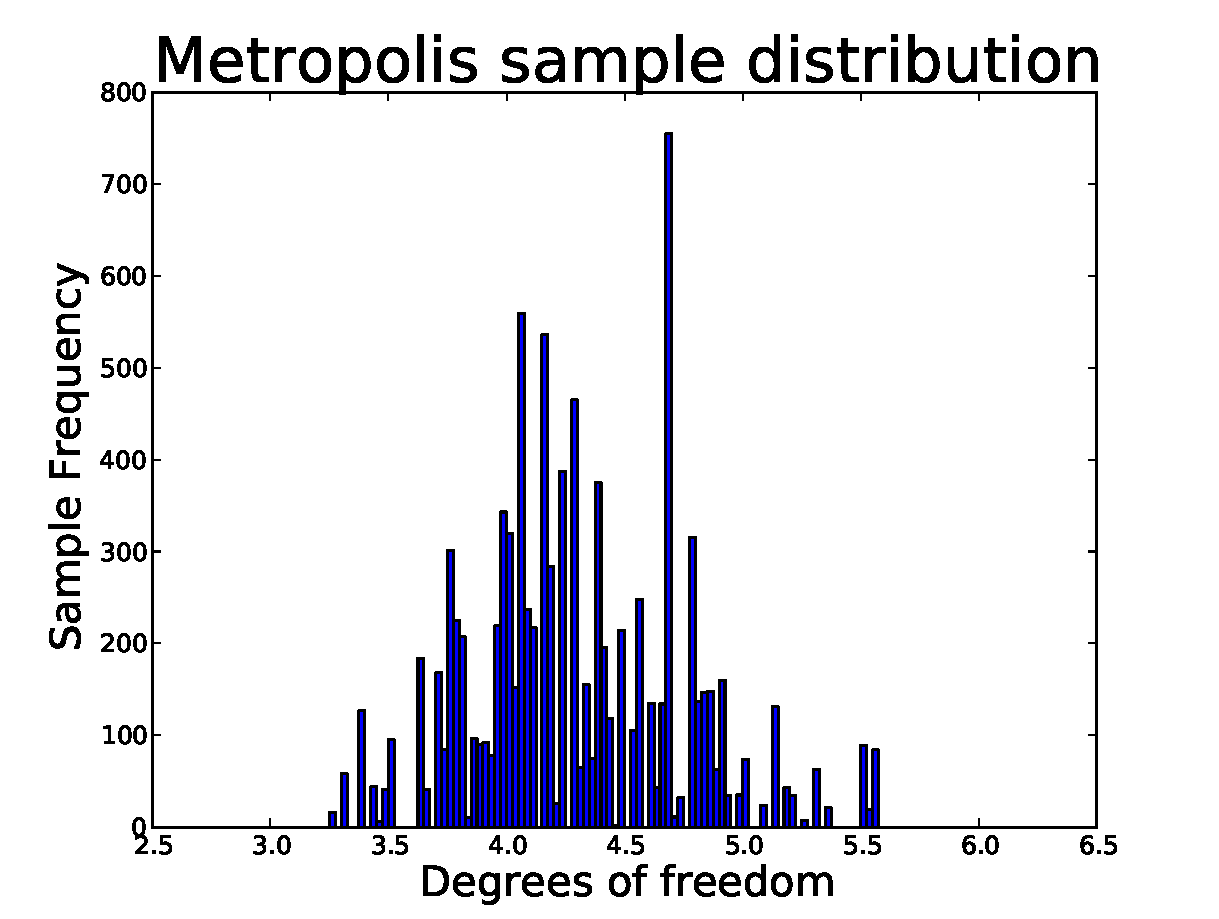
\includegraphics[width=\textwidth]{MetSampDist}
    \end{subfigure}
    ~
    \begin{subfigure}[t]{0.48\textwidth}
      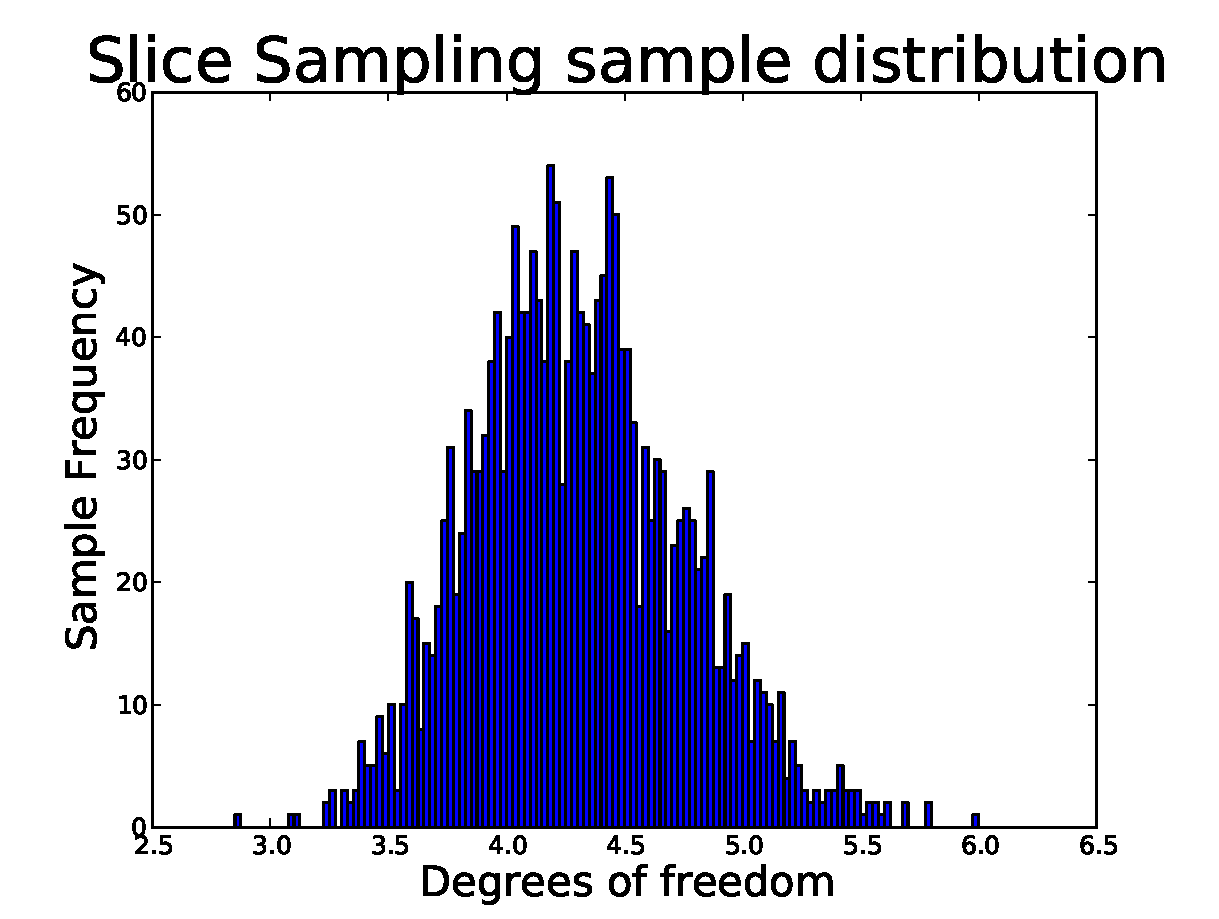
\includegraphics[width=\textwidth]{SliceSampDist}
    \end{subfigure}
    \caption{Empirical sample distribution of local metropolis and slice sampling on the Tdf continuous model}
    \label{fig:custSampDist}
\end{figure}

Based on these preliminary experiments slice sampling seems to confer a significant advantage over local metropolis when compared on the Tdf models.

\subsection{Generic, lightweight, slice sampling inference engine}

Since the custom slice sampling tests on the Tdf models gave promising results we next look at creating a generic slice sampling implementation that can run on arbitrary probabilistic programs. Our implementation, described in Section \ref{sect:StocPy}, follows the style of the PPLs presented in ``Lightweight Implementations of Probabilistic Programming Languages via Transformational compilation''. \todo{change this after bibliography exists}. 

The slice sampling technique we use follows the basic ideas presented in Section \ref{sect:sliceBack}. The main points are:
\begin{itemize}

\item
sample a height $u$ uniformly from $[0, likelihood]$. Since we are working with log likelihoods that are too small to be exponentiated, we take the sample directly in logspace by sampling from the exponential corresponding to the log of u. Specifically, if our log likelihood is ll, then $u \sim -1 * (exp(1) + ll)$

\item
uniformly sample a random variable $cur$ to modify

\item
find values $xl$ and $xr$ smaller and larger than the current value $x$ of the random variable $cur$ such that the log likelihood under $xl$ and $xr$ is smaller than the height $u$. Search for these values in an exponential fashion, by doubling the last guess.

\item
uniformly sample a proposition for $cur$ from (uniform $xl$ $xr$). Resample until the log likelihood under the sample is larger than the height $u$.

\end{itemize}

The stochastic python metropolis implementation presented in Section \ref{sect:StocPy} runs the Tdf continuous model 2-2.5x slower than the Venture implementation. The metropolis implementation also runs about 6x faster than slice-sampling, per number of samples. As discussed above, the bollteneck is the number of trace likelihood calculations. The metropolis method calculated the log-likelihood exactly once for each sample while slice sampling will execute it a minimum of 3 times (one each for $xl$, $xr$ and $x$). In practice, due to the stepping out and the possible resampling of a variable, we average 6 log-likelihood calculations per sample, thus explaining the 6x slow-down.

This shows that, for the tdf model, tweaking the initial width and interval search strategies as to reduce the number of log-likelihood calculations will result in a further improvement of no more than 2x.

\subsubsection{Slice sampling on the Tdf model}
We first run the 3 methods (my stochastic python metropolis and slice sampling implementations and Venture) for 10 minutes. The resulting distributions are shown in Figure \ref{fig:tdfSampDists}.

\begin{figure}[h]
        \centering
        \begin{subfigure}[b]{0.31\textwidth}
                \centering
                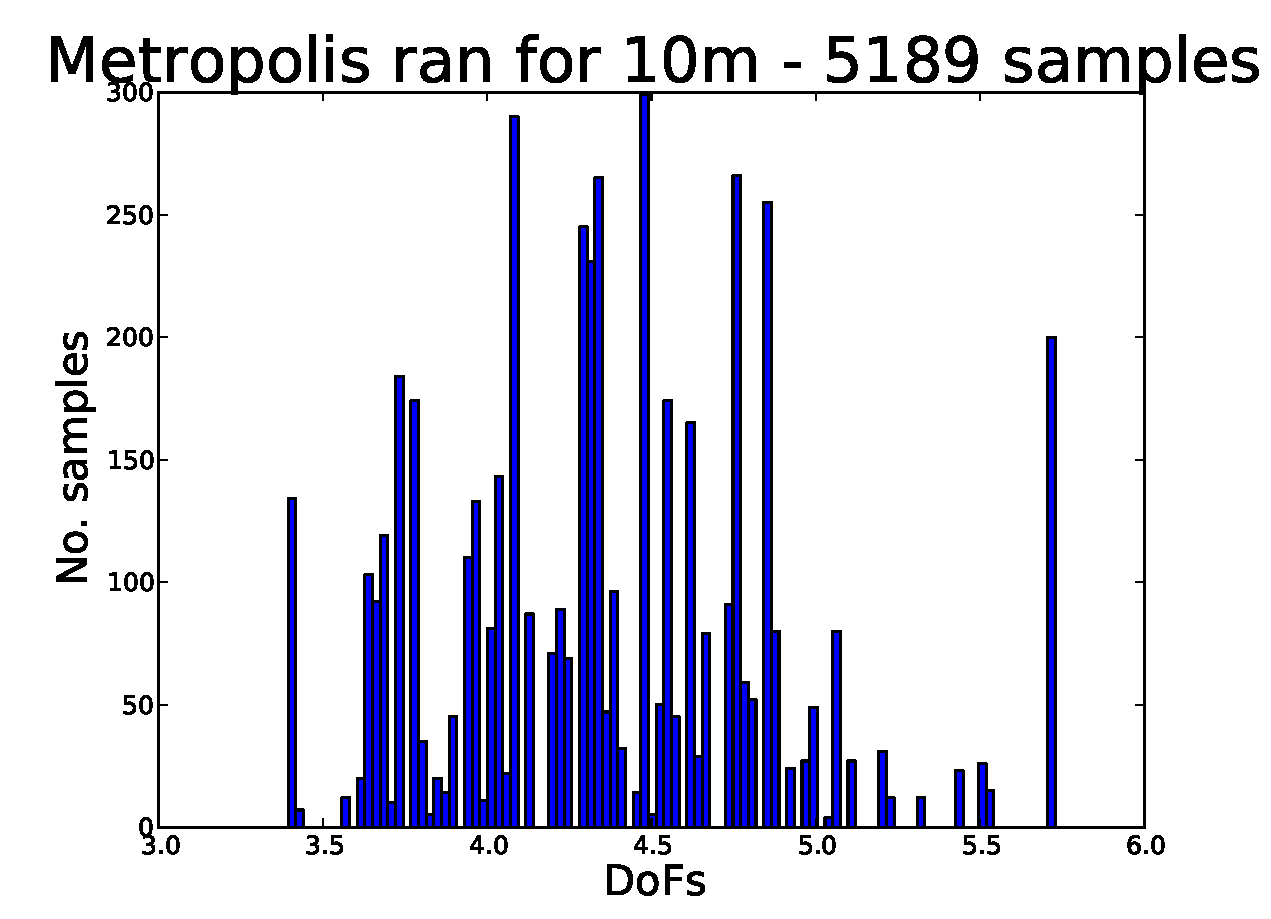
\includegraphics[width=\textwidth]{MetLISampDist}
        \end{subfigure}
        ~ 
        \begin{subfigure}[b]{0.31\textwidth}
                \centering
                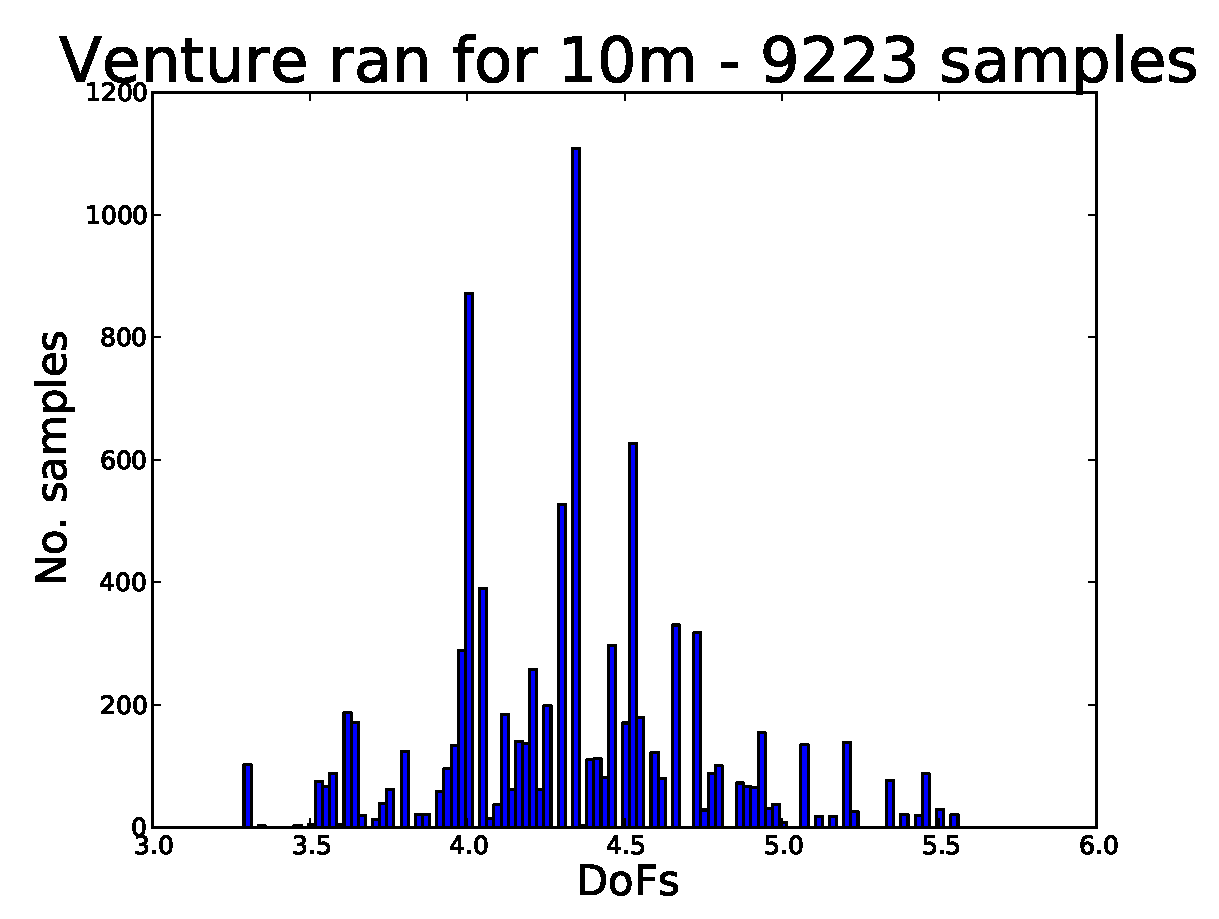
\includegraphics[width=\textwidth]{VentureLISampDist}
        \end{subfigure}
        ~ 
        \begin{subfigure}[b]{0.31\textwidth}
                \centering
                \includegraphics[width=\textwidth]{SliceLISampDist}
        \end{subfigure}
    \caption{Sample distribution from running Venture and stochastic python versions of metropolis and slice sampling for 10 minutes on the Tdf continuous model.}
    \label{fig:tdfSampDists}
\end{figure}

Visually, slice sampling appears to be doing the best job despite generating much fewer samples in 10 minutes than the other methods. In order to get a quantitative evaluation of the methods we can use the Kolmogorov-Smirnov statistic and plot a graph of the decreasing differences between the true cumulative distribution and the cumulative distributions inferred by the 3 methods. This experiment (see Figure \ref{fig:TdfSliceLIComp}) confirms our intuition and shows slice sampling significantly outperforming the other variants. 

\begin{figure}[h]
    \centering
    \includegraphics[width=0.8\textwidth]{TdfSliceLIComp}
    \caption{Comparison of Kolmogorov-Smirnov differences between true and inferred posteriors.}
    \label{fig:TdfSliceLIComp}
\end{figure}

\subsubsection{Slice sampling on gaussian mean inference models}
To further test the inference performance of metropolis and slice sampling I defined 3 models based on the problem of estimating the mean of a gaussian. The 3 models are and their posteriors are:

\noindent\begin{minipage}[t]{.32\textwidth}
\begin{flalign*}
  &NormalMean1: &
  \\ &\quad\quad m \sim N(0,1) &
  \\ &\quad\quad \text{observe }N(m,1) = 5 &
  \\ &\quad\quad \text{predict }m &
\end{flalign*}
\end{minipage}%
\begin{minipage}[t]{.32\textwidth}
\begin{flalign*}
  &NormalMean2: &
  \\ &\quad\quad m \sim N(0,1)
  \\ &\quad\quad v \sim invGamma(3,1)
  \\ &\quad\quad \text{observe }N(m,v) = 5
  \\ &\quad\quad \text{predict }m
\end{flalign*}
\end{minipage}%
\begin{minipage}[t]{.32\textwidth}
\begin{flalign*}
  &NormalMean3: &
  \\ &\quad\quad m \sim N(0,1)
  \\ &\quad\quad \text{if }m < 0
  \\ &\quad\quad\quad\quad v \sim invGamma(3,1)
  \\ &\quad\quad \text{else}
  \\ &\quad\quad\quad\quad v = 1/3
  \\ &\quad\quad \text{observe }N(m,v) = 5
  \\ &\quad\quad \text{predict }m
\end{flalign*}
\end{minipage}

\begin{figure}[h]
        \centering
        \begin{subfigure}[b]{0.31\textwidth}
                \centering
                \includegraphics[width=\textwidth]{Normal1Post}
        \end{subfigure}
        ~ 
        \begin{subfigure}[b]{0.31\textwidth}
                \centering
                \includegraphics[width=\textwidth]{Normal2Post}
        \end{subfigure}
        ~ 
        \begin{subfigure}[b]{0.31\textwidth}
                \centering
                \includegraphics[width=\textwidth]{Normal4Post}
        \end{subfigure}
    \caption{Analytically derived posteriors of the NormalMean1, NormalMean2 and NormalMean3 models.}
    \label{fig:tdfSampDists}
\end{figure}

We now look at the performance of metropolis, slice sampling and different mixtures of slice sampling and metropolis (with different mixing proportions) over the 3 NormalMean models. The mixture methods work by flipping a biased coin before extracting each sample in order to decide which inference method to use. Since slice sampling cannot handle trans-dimensional jumps, we dissalow such jumps in the mixture algorithms. These algorithms are therefore reliant on metropolis to switch between program traces with different numbers of variables. 

To compare the inference engines, we extract samples untill a certain number of trace likelihood calculations are performed and then repeat this process 100 times, in order to generate independent sample runs (starting from different random seeds). Figure \ref{fig:normal1Perf} shows both the runs and the quartiles of the runs on the first model.

\begin{figure}[h]
        \centering
        \begin{subfigure}[b]{0.48\textwidth}
                \centering
                \includegraphics[width=\textwidth]{Normal1Runs}
        \end{subfigure}
        ~ 
        \begin{subfigure}[b]{0.48\textwidth}
                \centering
                \includegraphics[width=\textwidth]{Normal1Quarts}
        \end{subfigure}
    \caption{Runs and quartiles generated by slice, metropolis and mixtures of metropolis and slice on the 1 dimensional NormalMean1 model.}
    \label{fig:normal1Perf}
\end{figure}

On the simple, 1d, model all variants of slice sampling clearly outperform metropolis. In the quartile graph we consider mixtures of metropolis and slice both with 10\% metropolis and with 50\% metropolis and find that the change doesn't have a significant impact on performance. This is likely because, if slice picks good samples, metropolis is likely to simply keep them unchanged (since it will tend to reject the proposal from the prior if they are worse).

\begin{figure}[h]
        \centering
        \begin{subfigure}[b]{0.48\textwidth}
                \centering
                \includegraphics[width=\textwidth]{Normal2Runs}
        \end{subfigure}
        ~ 
        \begin{subfigure}[b]{0.48\textwidth}
                \centering
                \includegraphics[width=\textwidth]{Normal2Quarts}
        \end{subfigure}
    \caption{Runs and quartiles generated by slice, metropolis and mixtures of metropolis and slice on the 2 dimensional NormalMean2 model.}
    \label{fig:normal2Perf}
\end{figure}

On the 2d model (see Figure \ref{fig:normal2Perf}), slice still clearly outperforms metropolis, though the gap is not as pronounced as for the 1d model. Further, as in the 1d model, the 3 different slice variants all get quite similar performance. Additionally, on this model, the fact that the slice mixtures get more samples per LL calculation translates into a slightly better performance for them than for the pure slice sampling method.

\begin{figure}[h]
        \centering
        \begin{subfigure}[b]{0.48\textwidth}
                \centering
                \includegraphics[width=\textwidth]{Normal4Runs}
        \end{subfigure}
        ~ 
        \begin{subfigure}[b]{0.48\textwidth}
                \centering
                \includegraphics[width=\textwidth]{Normal4Quarts}
        \end{subfigure}
    \caption{Runs and quartiles generated by slice, metropolis and mixtures of metropolis and slice on the trans-dimensional NormalMean3 model.}
    \label{fig:normal4Perf}
\end{figure}

The third model, seen in Figure \ref{fig:normal4Perf}, reveals several things worth noting. First of all, pure slice sampling does very badly. This is because the simple slice sampling algorithm used in this example cannot handle trans-dimensional probabilistic models, such as NormalMean3. We will look closer at this problem in Section \ref{sect:tdSlice}. Further, on this model, we see the first significant performance gap between the different mixtures of slice and metropolis. Since slice sampling cannot handle trans-dimensional jumps, one of the main purposes of the metropolis steps in the mixture model is to switch between program traces with different dimensionality. In the case of the 1:9 Metropolis:Slice mixture, we see that this dimensionality switch happens quite rarely, and so the markov chain is stuck on bad samples for long runs. The 1:1 mixture of slice sampling and metropolis, however, manages to switch dimensionality sufficiently often and thus outperforms pure metropolis.

\subsubsection{Branching Model}
\label{sect:branching}
In order to further test the slice sampling inference engine we look at the Branching model from the paper ``A New Approach to Probabilistic Programming Inference''. This is also a trans-dimensional model, but this time operating on discrete data. \todo{change this once bibliography exists} The model specification I use is:

\begin{align*}
  Branching3:
  \\& pois1 \sim Poisson(4)
  \\&\text{if }pois1 > 4
  \\&\quad x = 6
  \\&else
  \\&\quad pois2 \sim Poisson(4)
  \\&\quad x = fib(3 * pois1) + pois2 \tag{$fib$ is the fibonacci function}
  \\&\text{observe }Poisson(x) = 6
  \\&\text{predict }pois1
\end{align*}
\todo{mention the discrepancy with the paper?}

In order to test the convergence rate of the inference engines we must first analytically derive the true posterior for this model. This is given, up to values of 20 in Figure \ref{fig:BranchPost}.

\begin{figure}[h]
    \centering
    \includegraphics[width=0.8\textwidth]{BranchPost}
    \caption{True posterior for the Branching Model}
    \label{fig:BranchPost}
\end{figure}

In order to evaluate the engines, we use each to generate 100 independent sample runs, all performing an equal number of trace likelihood calculations. In Figure \ref{fig:branchPerf}, we plot the evolution of the KL divergences between the empirical and the true posterior as the number of trace likelihood calculations increase.

\begin{figure}[h]
        \centering
        \begin{subfigure}[b]{0.48\textwidth}
                \centering
                \includegraphics[width=\textwidth]{BranchRuns}
        \end{subfigure}
        ~ 
        \begin{subfigure}[b]{0.48\textwidth}
                \centering
                \includegraphics[width=\textwidth]{BranchQuarts}
        \end{subfigure}
    \caption{Runs and quartiles generated by slice, metropolis and mixtures of metropolis and slice on the Branching model.}
    \label{fig:branchPerf}
\end{figure}

As for the previous trans-dimensional model (NormalMode3), we see that the slice inference does not converge to the correct distribution since it cannot properly handle trans-dimensional jumps. The Metropolis:Slice mixtures do converge correctly but, on this model, are less efficient than the local Metropolis-Hastings.

One thing worth noting on this model, is that slice sampling proposes some values of pois1 that are extremely unlikely (such as 60). The reason it proposes these values is that it picks a slice height based on the trace log-likelihood which in this model can be extremely low due to the distribution of the conditioned upon variable (x). In the Branching model, likely values of the 2 random variables (based on their priors) can result in very unlikely program traces and these traces can then result in accepting very unlikely values of our 2 random variables, since the acceptance criterion is simply that the proposed trace have likelihood higher than a number drawn uniformly from [0, oldTraceLL]

However, we would expect this behaviour to only occur at the begining of a run, so the 1000 trace likelihood calculations burn-in period we are using should mitigate any influence this factor may have.

It's unclear why slice does worse on this model than on the NormalMean3 one, especially as the model distributions don't seem to affect the proposal efficiency, with both models averaging about 1 sample for 5 LL calculations. \todo{talk about the continuous vs. discrete aspect and the domain in which we expect slice to be good}

It is informative to look at a per sample comparison of metropolis and slice sampling (see Figure \ref{fig:branchPerfSamps}), in addition to the previous per trace likelihood comparison (even though slice does ``more work'' to generate a sample than metropolis). In this plot we can see that the samples generated by 1:1 Metropolis:Slice are actually slightly better than the pure metropolis ones. However the difference is not large enough to make up for the extra trace likelihood calculations that slice sampling must perform. We can also notice that the slice sampling mixtures experience a larger variance in performance than the pure metropolis method. This may be due to the fact that we are relying on only the metropolis generated samples to randomly switch between the 2 modes in the posterior.

\begin{figure}[h]
        \centering
        \begin{subfigure}[b]{0.48\textwidth}
                \centering
                \includegraphics[width=\textwidth]{BranchRunsSamps}
        \end{subfigure}
        ~ 
        \begin{subfigure}[b]{0.48\textwidth}
                \centering
                \includegraphics[width=\textwidth]{BranchQuartsSamps}
        \end{subfigure}
    \caption{Runs and quartiles generated by slice, metropolis and mixtures of metropolis and slice on the Branching model.}
    \label{fig:branchPerfSamps}
\end{figure}

\subsubsection{Trans-dimensional slice sampling}
\label{sect:tdSlice}
An interesting research question is whether (and how) it might be possible to modify the slice sampling algorithm so that it can correctly perform inference on probabilistic programs with varying numbers of dimensions.

As a pre-requisite to approaching this question, it is usefull to investigate what is going wrong when trying to perform inference on the Branching and NormalMean3 trans-dimensional models. On the Branching model investigated in Section \ref{sect:branching}, we see that the model has 2 random variables whose values determine the distribution of a 3rd variable which we condition on. This model is trans-dimensional since on different traces either one or both of the 2 variables will be sampled.

Re-writing the model so that both variables are always sampled, even if one of them is unused, leaves the posterior invariant. Therefore one method to correctly perform inference in a trans-dimensional model is to always sample all the variables that might ever be used in any trace. This approach will however be extremely inneficient in large models and is not a viable general solution. In Figure \ref{fig:branchTraceLik} we use this trick to see what the space of possible trace likelihoods looks like. Integrating out the pois2 variable from the above trace likelihood space results in the correct posterior distribution, shown in Figure \ref{fig:branchPost}).

\begin{figure}[h]
        \centering
        \begin{subfigure}[b]{0.48\textwidth}
                \centering
                \includegraphics[width=\textwidth]{BranchTraceLik}
                \caption{Space of trace likelihoods if both variables are always sampled.}
                \label{fig:branchTraceLik}
        \end{subfigure}
        ~ 
        \begin{subfigure}[b]{0.48\textwidth}
                \centering
                \includegraphics[width=\textwidth]{BranchPost}
                \caption{True posterior of Branching model.}
                \label{fig:branchPost}
        \end{subfigure}
\end{figure}

The issue with trans-dimensional jumps comes from the fact that the naive slice sampling algorithm will not sample the second poisson when it is not necessary, but will still think that the trace likelihoods between runs with different numbers of sampled variables are comparable. In doing so, the slice sampler will be pretending to be sampling from a 2D trace likelihood even when it really is 1D. The space of likelihoods implied by the naive slice sampling implementation is shown in Figure \ref{fig:branchWrongTraceLik}. Integrating out the pois2 variable from this incorrect likelihood space results in the implied posterior shown in Figrue \ref{fig:branchWrongPost}. This wrong posterior is the one which naive slice sampling will be attempting to infer. \todo{mention buggy metropolis version that also samples from this}

\begin{figure}[h]
        \centering
        \begin{subfigure}[b]{0.48\textwidth}
                \centering
                \includegraphics[width=\textwidth]{BranchWrongTraceLik}
                \caption{Space of trace likelihoods if both variables are always sampled.}
                \label{fig:branchWrongTraceLik}
        \end{subfigure}
        ~ 
        \begin{subfigure}[b]{0.48\textwidth}
                \centering
                \includegraphics[width=\textwidth]{BranchWrongPost}
                \caption{Space of trace likelihoods implied by naive slice sampling.}
                \label{fig:branchWrongPost}
        \end{subfigure}
\end{figure}

Next we'll look at one simple attempt to correct for trans-dimensional jumps, by thinking in terms of fresh and stale likelihoods, as in the metropolis acceptance ratio. We define a variable as being stale if it was used in the previous program trace but not in the current one. Conversely, a variable is considered fresh if it is being sampled in the current trace but was not used in the previous one. The correction we propose means that, ehen comparing a trace log-likelihood against the slice's sampled height, we won't simply consider the log likelihood (ll), but instead ll + llStale - llFresh.

This correction means that when we are considering a jump to a lower dimensional space the log-likelihood of the lower dimensional space will be decreased by llStale (i.e. the likelihoods of the variables which are not part of this space). Conversely, when considering a move to a higher dimensional space, the log-likelihood of the higher-dimensional trace will be discounted by llFresh (so only the likelihood of the subset of variables that are also part of the current, lower-dimensional, space count). This simple correction seems to give correct results on the continuous NormalMean3 trans-dimensional model explored above (see Figure \ref{fig:normal4TD}).

\begin{figure}[h]
        \centering
        \begin{subfigure}[b]{0.48\textwidth}
                \centering
                \includegraphics[width=\textwidth]{Normal4TDRuns}
        \end{subfigure}
        ~ 
        \begin{subfigure}[b]{0.48\textwidth}
                \centering
                \includegraphics[width=\textwidth]{Normal4TDQuarts}
        \end{subfigure}
    \caption{Runs and quartiles generated by metropolis, a mixture of metropolis and slice, and both the modified and the naive slice algorithms on the NormalMean3 model.}
    \label{fig:normal4TD}
\end{figure}

However, the specification appears to be wrong since it does not converge to the correct distribution on the Branching model (see Figure \ref{fig:branchTD}). Somewhat interestingly, it does seem to converge to a wrong value that's somewhat closer to the true posterior than the naive slice sampling does.

\begin{figure}[h]
        \centering
        \begin{subfigure}[b]{0.48\textwidth}
                \centering
                \includegraphics[width=\textwidth]{BranchTDRuns}
        \end{subfigure}
        ~ 
        \begin{subfigure}[b]{0.48\textwidth}
                \centering
                \includegraphics[width=\textwidth]{BranchTDQuarts}
        \end{subfigure}
    \caption{Runs and quartiles generated by metropolis, a mixture of metropolis and slice, and both the corrected slice and the naive slice algorithms on the Branching model.}
    \label{fig:branchTD}
\end{figure}

\section{Quasi-Monte Carlo}
Another possible improvement on naive MC is, rather than sampling randomly from the unit interval, to instead make use of a low-discrepancy sequence that will tend to cover the interval faster.

A simple sequence we can use in the 1-dimensional case is the Van der Corput sequence.
We test the performance of this sequence by considering time to mode of neighbourhood for a interval of size 100, neighbourhood of size 1 and modes in the range $[0.5, 1.5, \ldots 99.5]$
Naive metropolis will find this neighbourhood, on average in 100 steps. Using the Van der Corput sequence reduces this to 56 samples. 

The slice sampling technique explored above, however,  managed reductions to 10 and 20 steps respectively (depending on the likelihood function). Therefore I choose to focus on developing the slice sampling technique rather than further investigation Quasi-Monte Carlo methods.



\chapter{Summary and Conclusions} 

As you might imagine: summarizes the dissertation, and draws 
any conclusions. Depending on the length of your work, and 
how well you write, you may not need a summary here. 

You will generally want to draw some conclusions, and point
to potential future work. 


\appendix
\singlespacing

\bibliographystyle{unsrt} 
%\bibliography{dissertation} 

\end{document}
